\documentclass[10pt]{article}
\usepackage{fullpage}

\usepackage{fontspec}          % Assumes you're using xelatex
\setmainfont{Times New Roman}

\usepackage{fancybox}  % Must include fancybox *before* fancyvrb; don't know why.
\usepackage{fancyvrb}
\usepackage{graphicx}
\usepackage[usenames,dvipsnames]{color}
\usepackage[backref,colorlinks]{hyperref}
\usepackage[authoryear]{natbib}

\hypersetup{
  citecolor = {RoyalBlue},
  linkcolor = {RoyalBlue},
  urlcolor  = {RoyalBlue},
}


\setcounter{secnumdepth}{1}

% customizations used in the User's Guide

\newenvironment{wideitem}{\begin{list} 
     {}
     { \setlength{\labelwidth}{2in}\setlength{\leftmargin}{1.5in}}}
     {\end{list}}

\newenvironment{miditem}{\begin{list} 
     {}
     { \setlength{\labelwidth}{1.5in}\setlength{\leftmargin}{1in}}}
     {\end{list}}

% need temp vars for parindent, parskip saving
%
\newlength{\sresavei}
\newlength{\sresaves}

% Consistent font styles
%   \prog{}  for a program or file name
%   \emprog{} for an emphasized program or file name
%   \user{}     for a typed used command
%   \begin{machine}  for machine output

\newcommand{\prog}[1]{\texttt{#1}}
\newcommand{\emprog}[1]{{\bfseries\texttt{#1}}}
\newcommand{\user}[1]{\noindent{\small\bfseries\texttt{$>$ #1}}\\}

\newenvironment{machine}
  {\small\ttfamily\begin{verbatim}}
  {\end{verbatim}}
   

\begin{document}
\bibliographystyle{apalike}

\begin{titlepage}
{\Large

\vspace*{\fill}

\begin{latexonly}
\noindent
{\Huge \textsf{HMMER User's Guide}} \\ 
\rule[2pt]{\textwidth}{1pt} \\
\hspace*{\fill} {\large \textsf{Biological sequence analysis using
profile hidden Markov models} \\ }
\end{latexonly}

\begin{htmlonly}
\begin{center}
{\Huge \textbf{HMMER User's Guide}}\\
{\large \textbf{Biological sequence analysis using
profile hidden Markov models}}\\
\end{center}
\end{htmlonly}

\vspace*{\fill}

\begin{center}
\textsl{\htmladdnormallink{http://hmmer.wustl.edu/}{http://hmmer.wustl.edu/}}\\
Version 2.2; August 2001 \\ 

\vspace*{\fill}

Sean Eddy\\
Howard Hughes Medical Institute and Dept. of Genetics\\
Washington University School of Medicine\\
660 South Euclid Avenue, Box 8232\\
Saint Louis, Missouri 63110, USA\\
\textsl{eddy@genetics.wustl.edu} \\
With contributions by Ewan Birney (\textsl{birney@sanger.ac.uk})\\
\end{center}

\vspace*{\fill}

}
\end{titlepage}

\vspace*{\fill}
\begin{flushleft}
Copyright (C) 1992-2001, Washington University in St. Louis.\vspace{5mm}

Permission is granted to make and distribute verbatim copies of this
manual provided the copyright notice and this permission notice are
retained on all copies.\vspace{5mm}

The HMMER software package is a copyrighted work that may be freely
distributed and modified under the terms of the GNU General Public
License as published by the Free Software Foundation; either version 2
of the License, or (at your option) any later version. Some versions
of HMMER may have been obtained under specialized commercial licenses
from Washington University; for details, see the files COPYING and
LICENSE that came with your copy of the HMMER software.\vspace{5mm}

This program is distributed in the hope that it will be useful, but
WITHOUT ANY WARRANTY; without even the implied warranty of
MERCHANTABILITY or FITNESS FOR A PARTICULAR PURPOSE.\vspace{5mm}

See the Appendix for a copy of the full text of the GNU General Public
License.\vspace{5mm}

\end{flushleft}

\newpage
\tableofcontents

\newpage
\section{Introduction}

If you just want to get started fast, skip this section and go
straight to the installation instructions, then to the tutorial.

\subsection{What does HMMER do?}

You discover a new protein sequence family, and carefully construct a
multiple sequence alignment. Your family, like most protein families,
has a number of strongly (but not absolutely) conserved key residues,
separated by characteristic spacing. You wonder if there are more
members of your family in the sequence databases, but the family is so
evolutionarily diverse, a BLAST search with any individual sequence
doesn't even find the rest of the sequences you already know about;
you're sure there are some distantly related sequences in the
``noise''. You spend many pleasant evenings scanning weak BLAST
alignments by eye to find ones with the right key residues are in the
right places. You sure wish there was a computer program that did this
better.

You get the sequence of another favorite protein and eagerly BLAST it
against the NCBI server, and nothing significant shows up. It looks
like you'll get no easy information from the sequence.

You BLAST another favorite sequence against the NCBI server; a
thousand hits come back, and the top hundred are hypothetical
sequences from genome projects. It looks like you'll have to wade
through a lot of BLAST output to find the informative hits.

Another sequence comes back a slew of hits to receptor tyrosine
kinases, but before you decide to call your sequence an RTK homologue,
you recall that RTK's are, like many proteins, composed of multiple
functional domains. Is your sequence really an RTK? Or is it a novel
sequence that also happens to have a protein kinase catalytic domain,
fibronectin type III domain, or immunoglobulin superfamily domain?

These (and other problems in sequence analysis) are the kinds of
problems that HMMER tries to address. HMMER works with consensus
statistical models of multiple sequence alignments, called
\emph{profile hidden Markov models} (profile HMMs).

\subsection {Profile HMMs}

Profile hidden Markov models (profile HMMs) are statistical models of
the primary structure consensus of a sequence family. Anders Krogh,
David Haussler, and co-workers at UC Santa Cruz introduced profile
HMMs \cite{Krogh94}, adopting HMM techniques which have been used for
years in speech recognition. HMMs had been used in biology before the
Krogh/Haussler work, but the Krogh paper had a particularly dramatic
impact, because HMM technology was so well-suited to the popular
``profile'' methods for searching databases using multiple sequence
alignments instead of single query sequences. Since then, several
computational biology groups (including ours) have rapidly adopted
HMMs as the underlying formalism for sequence profile analysis.

``Profiles'' were introduced by Gribskov and colleagues
\cite{Gribskov87,Gribskov90} at about the same time
that other groups introduced similar approaches, such as ``flexible
patterns'' \cite{Barton90}, and
``templates''\cite{Bashford87,Taylor86}. The term ``profile'' has
stuck.\footnote{There has been some agitation to call all such models
``position specific scoring matrices'', PSSMs, but certain small
nocturnal North American marsupials have a prior claim on the
mnemonic.}  All of these are more or less statistical descriptions of
the consensus of a multiple sequence alignment. They use
position-specific scores for amino acids (or nucleotides) and position
specific scores for opening and extending an insertion or deletion.
Traditional pairwise alignment (for example, BLAST
\cite{Altschul90}, FASTA \cite{Pearson88}, or the Smith/Waterman
algorithm \cite{Smith81}) uses position-{\em independent} scoring
parameters. This property of profiles captures important information
about the degree of conservation at various positions in the multiple
alignment, and the varying degree to which gaps and insertions are
permitted.

The advantage of using HMMs is that HMMs have a formal probabilistic
basis. We can use Bayesian probability theory to guide how all the
probability (scoring) parameters should be set. Though this might
sound like a purely academic issue, this probabilistic basis lets us
do things that the more heuristic methods cannot do easily. For
example, an HMM can be trained from unaligned sequences, if a trusted
alignment isn't yet known. Another consequence is that HMMs have a
consistent theory behind gap and insertion scores.\footnote{
Surprisingly, this is still controversial.  People have been saying
``there is no theory for setting gap scores'' for so long that many
people believe it.} In most details, HMMs are a slight improvement
over a carefully constructed profile -- but far less skill and manual
intervention is necessary to train a good HMM and use it.  This allows
us to make libraries of hundreds of profile HMMs and apply them on a
very large scale to whole-genome or EST sequence analysis.  One such
database of protein domain models is Pfam \cite{Sonnhammer97}; the
construction and use of Pfam is tightly tied to the HMMER software
package.

HMMs do have important limitations. One is that HMMs do not capture
any higher-order correlations.  An HMM assumes that the identity of a
particular position is independent of the identity of all other
positions.\footnote{This is not strictly true. There is a subtle
difference between an HMM's state path (a first order Markov chain)
and the sequence described by an HMM (generated from the state path by
independent emissions of symbols at each state).} HMMs make poor
models of RNAs, for instance, because an HMM cannot describe base
pairs. Also, compare protein ``threading'' methods, which include
scoring terms for nearby amino acids in a three-dimensional protein
structure. 

A general definition of HMMs and an excellent tutorial introduction to
their use has been written by Rabiner \cite{Rabiner89}. Throughout, I
will often use ``HMM'' to refer to the specific case of profile HMMs
as described by Krogh et al. \cite{Krogh94}. This shorthand usage is
for convenience only. For a review of profile HMMs, see \cite{Eddy96},
and for a complete book on the subject of probabilistic modeling in
computational biology, see \cite{Durbin98} 
\begin{htmlonly}
\htmladdnormallink{[More information on-line]}
{http://www.genetics.wustl.edu/eddy/publications/cupbook.html}
\end{htmlonly}.

\subsection{Primary changes from HMMER 1.x}

HMMER 2 is an almost complete rewrite of the original 1992-1996 HMMER
code. A list of the major changes follows.

\begin{wideitem}

\item [\textbf{Plan7}] The model architecture is changed. The ``Plan 7''
architecture\footnote{The origin of the codename is obscure, involving
both details of the state transition probability distributions in
profile HMM architecture and an inordinate fondness for bad science
fiction movies. Frighteningly, David Haussler understood the codename
immediately.} allows detailed control over parameters of local,
global, and multidomain alignments. In Plan 7, you choose the
alignment style when you build the model with \prog{hmmbuild}, not
when you search. A single database search program \prog{hmmsearch}
replaces the four search programs in HMMER 1.x.

\item [\textbf{Pfam support}] There is much better support for the Pfam
HMM database. HMMs have names; the HMM file format allows libraries of
multiple HMMs per file; and there is a search program
\prog{hmmpfam}
for searching a single query sequence against an HMM library.
HMM databases like Pfam can be indexed for rapid access using
\prog{hmmindex}, and single HMMs can be retrieved from an HMM
database using \prog{hmmfetch}.

\item [\textbf{E-values}] HMMER now reports both log-odds scores and
a E-value. E-values can detect significant matches even when the
log-odds score is negative. A new program \prog{hmmcalibrate}
empirically determines the necessary parameters for estimating
E-values as best as possible.

\item [\textbf{Output}] Database searches now sort and postprocess their results for
prettier and more useful output. Output styles are deliberately
similar to BLAST, to try to simplify the design of postprocessors.

\item [\textbf{Save file format}] HMMER save files are now in an ASCII format which
  is easy for humans to read, portable across all architectures
  without byteswapping issues, and compact.

\item [\textbf{Decent defaults}] The ``best'' average behavior of HMMER is now its
default behavior. For example, mixture Dirichlet priors are now the
default for protein model building. In HMMER 1.x, you had to invoke a
number of ``experimental'' options to get better performance -- this
led to a bunch of really frustrating benchmarking in the literature,
in which people compared fully optimized program X to the default
behavior of HMMER 1, which was the 1994 basic Krogh/Haussler behavior
rather than its actual power. (However, there's still a lot of bad
benchmarking, because people don't understand how to benchmark profile
software yet.)

\end{wideitem}

\subsection{Plan 7}

\subsubsection{The Plan 7 architecture}

The Plan 7 architecture is substantially different from the original
HMMER model architecture. 

The abbreviations for the states are as follows:

\begin{wideitem}
\item [\textbf{M$_x$}] Match state $x$.  Has $K$ emission probabilities.
\item [\textbf{D$_x$}] Delete state $x$. Non-emitter.
\item [\textbf{I$_x$}] Insert state $x$. Has $K$ emission probabilities.
\item [\textbf{S}]     Start state. Non-emitter.
\item [\textbf{N}]     N-terminal unaligned sequence state. 
    Emits \textit{on transition} with $K$ emission probabilities.
\item [\textbf{B}]     Begin state (for entering main model). Non-emitter.
\item [\textbf{E}]     End state (for exiting main model). Non-emitter.
\item [\textbf{C}]     C-terminal unaligned sequence state.
    Emits \textit{on transition} with $K$ emission probabilities.
\item [\textbf{J}]     Joining segment unaligned sequence state.
    Emits \textit{on transition} with $K$ emission probabilities.
\end{wideitem}

\begin{figure}
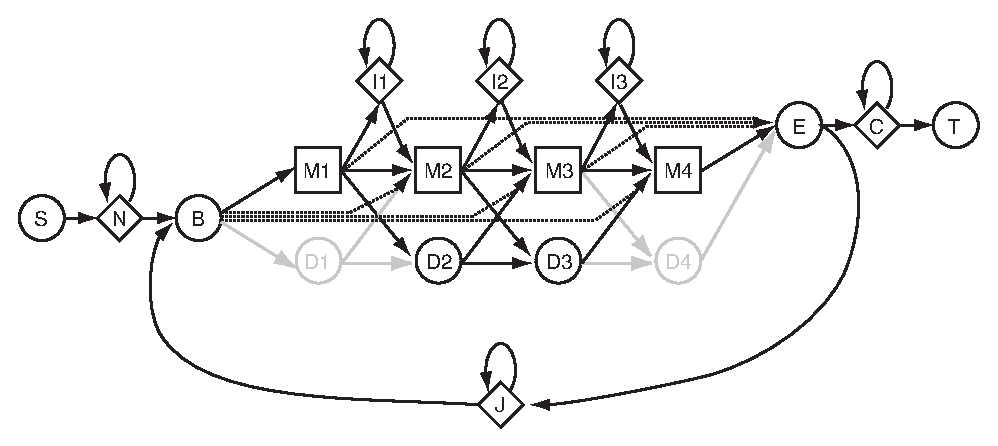
\includegraphics{plan7}
\caption{\textit{The Plan7 architecture. Squares indicate match states
(modeling consensus positions in the alignment). Diamonds indicate
insert states (modeling insertions relative to consensus) and special
random sequence emitting states. Circles indicate delete states
(modeling deletions relative to consensus) and special begin/end
states. Arrows indicate state transitions. See text for more details.}}
\end{figure}

The section of the model composed of M, D, and I states, and the B and
E states, is essentially a Krogh/Haussler profile HMM. I refer to this
as the ``main model''. A group of three states M/D/I at the same
consensus position in the alignment is called a ``node''. The main
model controls the \textit{data dependent} features of the model.  The
probability parameters in the main model are generally learned from
data in a multiple sequence/structure alignment.

Unlike the original Krogh/Haussler and HMMER model architecture, Plan
7 has no D $\rightarrow$ I or I $\rightarrow$ D transitions. This
reduction from 9 to 7 transitions per node in the main model is the
origin of the codename Plan 7. (The original HMMER architecture is
called Plan 9 in parts of the code.)

The other states (S,N,C,T,J) are called ``special states''. They
(combined with special entry probabilities from B and exit
probabilities to E) control the \textit{algorithm dependent} features
of the model: how likely the model is to generate various sorts of
local or multihit alignments. The algorithm dependent parameters are
typically not learned from data, but rather set externally by choosing
a desired alignment style.

\subsubsection{Local alignments in Plan 7}

The Plan 7 architecture models a complete sequence, regardless of how
much of that sequence matches the main model. \textit{All alignments
to a Plan 7 model are ``global'' alignments}, but some of the sequence
may be assigned to Plan 7 states (N,C,J) that generate ``random''
sequence that is not aligned to the main model.  Thus, the algorithm
dependent parts of the model control the \textit{apparent} locality of
the alignments.

Local alignments with respect to the sequence (i.e., allowing a match
to the main model anywhere internal to a longer sequence) are
controlled by the N and C states. If the N $\rightarrow$ N transition
is set to 0, alignments are constrained to start in the main model at
the very first residue. Similarly, if the C $\rightarrow$ C transition
is set to 0, alignments are constrained to match the main model at the
very last residue in the sequence.

Local alignments with respect to the model (i.e., allowing fragments
of the model to match the sequence) are controlled by B $\rightarrow$
M ``entry'' transitions and M $\rightarrow$ E ``exit'' transitions,
shown as dotted lines in the Plan 7 figure. Setting all entries but
the B $\rightarrow$ M$_1$ transition to 0 forces a partially
``global'' alignment in which all alignments to the main model must
start at the first match or delete state. Setting all exits to 0 but
the final M $\rightarrow$ E transition (which is always 1.0) forces a
partially global alignment in which all alignments to the main model
must end at the final match or delete state.

Multiple hit alignments are controlled by the E $\rightarrow$ J
transition and the J state. If the E $\rightarrow$ J transition is set
to 0, a sequence may only contain one domain (one alignment to the
main model). If it is nonzero, more than one domain per sequence can
be aligned to the main model. The J $\rightarrow$ J transition
controls the expected length of the intervening sequence between
domains; the lower this probability, the more clustered the domains
are expected to be.

The original HMMER1 search programs are encoded in Plan 7 models as
follows:

\begin{wideitem}
\item [\emprog{hmms}] Simple global alignment. $t_{NN}$ and $t_{CC}$ set to
$t_{GG}$ from the null model (see below). $t_{EJ}$ set to
zero. Internal entries and exits set to zero.

\item [\emprog{hmmls}] Akin to ``profile'' alignment (as Waterman and others
call it): global with respect to main model, local with respect to
sequence, multiple nonoverlapping domains allowed. $t_{NN}$ and
$t_{CC}$ set to $t_{GG}$ from the null model. $t_{EJ}$ set to
0.5. Internal entries and exits set to zero.
 
\item [\emprog{hmmsw}] Smith/Waterman alignment: fully local with 
respect to both the main model and the sequence; single domain.
$t_{NN}$ and $t_{CC}$ set to $t_{GG}$ from the null model. $t_{EJ}$
set to zero. Internal entries are set to $0.5/(M-1)$ for a model with
$M$ match states. Exit probabilities are set such that the overall
chance of exiting from an internal match state is 0.5, and the
posterior probability distribution over which match state is exited is
equal (I'm trying to word this carefully; the M $\rightarrow$ E
probabilities are not equal, because there's a small compensation for
the fact that if you can leave from $M_5$, then the chance that you'll
even get to $M_6$ is reduced.)

\item [\emprog{hmmfs}] Multihit Smith/Waterman alignment. Same
as the above, but $t_{EJ}$ is set to 0.5.
\end{wideitem}


One advantage of Plan 7 is great flexibility in choosing an alignment
style. Complicated alignment styles are easily encoded in the model
parameters without changing the alignment algorithm.  For example, say
you wanted to model human L1 retrotransposon elements. Because of the
way L1 elements are inserted by reverse transcriptase (RVT), L1
elements tend to have a defined 3' end (RVT starts replication at the
same place in each new L1) but a ragged 5' end (RVT prematurely falls
off a new L1 in an unpredictable fashion). A specialized L1 model
could define non-zero internal entry probabilities and zero internal
exit probabilities to model this biological situation.

One disadvantage of Plan 7 is that if you decide you want to do both
local and global alignments, you need two different models (or you
need to do one search, then change the model). This wouldn't be a
terrible burden except for the fact that the algorithm-dependent
parameters strongly affect the values of the $\mu$ and $\lambda$
parameters that E-value statistics depend on. If the algorithm
dependent parameters are changed, these parameters are lost and the
model should be recalibrated with \prog{hmmcalibrate} -- and
\prog{hmmcalibrate} is relatively slow.


\subsubsection{The Plan 7 null model}

When HMM alignments are scored, they are scored by a log-odds score
relative to a ``null model'' of random sequence composition
\cite{Barrett97}. In Plan 7, this model is now specified as a full
probabilistic model too:

\begin{center}
\includegraphics{nullmodel}
\end{center}

The G state has a symbol emission probability distribution for $K$
symbols in the alphabet. By default, this distribution is set either
to the average amino acid composition of SWISSPROT 34, or to 0.25 for
each nucleotide. The G $\rightarrow$ G transition controls the
expected length of observed random sequences; in practice, this
transition probability is so close to 1 that it has very little
effect. The F state is just a dummy end state like the T state in the
Plan 7 architecture.

\subsubsection{Wing retraction in Plan 7 dynamic programming}

In the figure of the Plan 7 architecture, you may have noticed that
the first and last delete states are greyed out. Internally in HMMER,
these delete states exist in the ``probability form'' of the model
(when the model is being worked with in every way except alignments)
but they are carefully removed in the ``search form'' of the model
(when the model is converted to log-odds scores and used for
alignments). This process is called ``wing retraction'' in the code,
by analogy to a swept-wing fighter changing from a wings-out takeoff
and landing configuration to a wings-back configuration for high speed
flight.

The problem is that the Plan 7 model allows cycles through the J
state. If a continuous nonemitting ``mute cycle'' were possible (J, B,
D states, E, and back to J), dynamic programming recursions would
fail. This is why special mute states like delete states must be
handled carefully in HMM dynamic programming algorithms; see
\cite{Durbin98} for further discussion. The easiest way to
prevent a mute cycle is to make sure that the model must pass through
at least one match state per path through the main model.

Wing retraction involves folding the probabilities of the terminal
delete paths into the Plan 7 entry and exit probabilities. For
example, in wing retraction the ``algorithm dependent'' B
$\rightarrow$ M$_{3}$ entry probability is incremented by the
probability of the ``data dependent'' path B $\rightarrow$ D$_1$
$\rightarrow$ D$_2$ $\rightarrow$ M$_3$.

Having the wing retraction step, rather than {\em always} folding
these probabilities together, is a design decision, preserving a
distinction between the ``algorithm dependent'' and ``data dependent''
parts of the model.

\subsection{Sequence file formats}

For all the programs, unaligned sequence files can be in FASTA,
Genbank, EMBL, or SWISS-PROT format, as well as a few other common
file formats. The programs automatically detect what format the file
is in and whether the sequences are DNA, RNA, or protein.

Aligned sequence files can be in ClustalW, GCG MSF, or SELEX
format. SELEX format is a simple format of one line per sequence,
containing the name first, followed by the aligned sequence. ClustalW,
MSF and SELEX alignment files can also be used where unaligned format
files are required; the sequences will be read in and their gaps
removed. 

Full specifications of these file formats and the other formats
recognized by the HMM package are in the file formats chapter near the
end of the guide.

The programs work on RNA, DNA, and protein sequence. They
automatically detect what your sequences are. The behavior of the
programs when a nucleic acid model is used to analyze protein
sequences, or vice versa, is undefined. Certain other situations may
arise (trying to search the ``complementary strand'' of a protein
database, for example) that are nonsensical in certain contexts. Be
forewarned. If you're lucky, the software will issue a snide warning
to you if you try to do something nonsensical, but usually it will
assume you know what you're doing.

\subsection{Command line options}

If you forget the command-line syntax or available options of any of
the programs, you can type the name of the program with no other
arguments and get a short help message, including summaries of the
common options.

Commonly used options are generally small letters, like \prog{-a}.
More infrequently used options are generally large letters, like
\prog{-A}. Expert or experimental options are generally in the GNU long form,
like \prog{--null2}.

If you call any program with an option {\tt -h}, you get an augmented
help message, including version info (the software version number is
helpful if you report bugs or other problems to me) and a complete
summary of all the available options, including rarely used and
expert/experimental ones.

\subsection{Environment variables}

HMMER is built to coexist peacefully with the BLAST suite of database
search programs \cite{Altschul91}. HMMER reads the following
environment variables (the examples given use UNIX csh syntax):

\begin{wideitem}
\item [\emprog{BLASTDB}] Location of sequence databases that
	\prog{hmmsearch} will look in, in addition to the current
	working directory.
	Multiple directories are allowed, separated by colons. A
	trailing slash on each path is important to BLAST, but not to HMMER.\\
	Examples: \\
	\user{setenv BLASTDB /nfs/databases/}
        \user{setenv BLASTDB /nfs/databases/:/nfs/moredatabases/}

\item [\emprog{BLASTMAT}] Location of substitution matrices that
	\prog{hmmbuild --pam} (the PAM prior option) can read.
	Although HMMER can parse a colon-separated list, BLAST must
	have a single directory path here.
	Example:\\
	\user{setenv BLASTMAT /nfs/databases/matrix/}

\item [\emprog{HMMERDB}] Location of HMMs, PFAM, or other HMMER
	specific data files. Any program that reads an HMM file
	looks in both HMMERDB and the current working directory.
	Multiple directories are allowed, colon-separated.
	Examples:\\
	\user{setenv HMMERDB /usr/local/lib/hmmer/}
	\user{setenv HMMERDB /usr/local/lib/hmmer/:/nfs/databases/pfam/}

\item [\emprog{HMMER\_NCPU}] On multiprocessors that support POSIX
	threads (this includes almost all modern UNIX multiprocessors;
	for example, SGI Origin servers), the programs
	\prog{hmmcalibrate}, \prog{hmmpfam}, and \prog{hmmsearch}
	run as parallelized, multithreaded applications.
	Normally they will take over all available CPUs in the machine.
	HMMER\_NCPU sets a maximum number of CPUs to utilize,
	so HMMER searches are ``good citizens'', leaving some
 	CPU power for other jobs. An example of configuring
	HMMER to use only 16 processors on a 32-processor Origin:\\
	\user{setenv HMMER\_NCPU 16}
\end{wideitem}

\subsection{Other profile HMM implementations}

Several implementations of profile HMM methods and related PSSM
methods are available.  Some are listed in the table below.

\begin{center}
\begin{tabular}{ll}
Software  &   URL \\ \hline
HMMER     & \htmladdnormallink{http://hmmer.wustl.edu/}{http://hmmer.wustl.edu/}  \\
SAM       & \htmladdnormallink{http://www.cse.ucsc.edu/research/compbio/sam.html}{http://www.cse.ucsc.edu/research/compbio/sam.html} \\
PFTOOLS   & \htmladdnormallink{http://ulrec3.unil.ch:80/profile/}{http://ulrec3.unil.ch:80/profile/}  \\
HMMpro    & \htmladdnormallink{http://www.netid.com/html/hmmpro.html}{http://www.netid.com/html/hmmpro.html}\\
GENEWISE  & \htmladdnormallink{http://www.sanger.ac.uk/Software/Wise2/}{http://www.sanger.ac.uk/Software/Wise2/} \\
PROBE     & \htmladdnormallink{ftp://ncbi.nlm.nih.gov/pub/neuwald/probe1.0/}{ftp://ncbi.nlm.nih.gov/pub/neuwald/probe1.0/} \\
META-MEME & \htmladdnormallink{http://www.cse.ucsd.edu/users/bgrundy/metameme.1.0.html}{http://www.cse.ucsd.edu/users/bgrundy/metameme.1.0.html} \\
BLOCKS    & \htmladdnormallink{http://www.blocks.fhcrc.org/}{http://www.blocks.fhcrc.org/} \\
PSI-BLAST & \htmladdnormallink{http://www.ncbi.nlm.nih.gov/BLAST/newblast.html}{http://www.ncbi.nlm.nih.gov/BLAST/newblast.html} \\
\end{tabular}
\end{center}

HMMER, SAM, PFTOOLS, and HMMpro are the most closely related to the
profile HMM methods introduced by Krogh et al. HMMpro is commercial,
not free software.


\newpage
\section{Installation}
\label{section:installation}
\setcounter{footnote}{0}

\subsection{Quick installation instructions}

Download \prog{hmmer-3.0b3.tar.gz} from
\url{http://hmmer.org/}, or directly from
\url{ftp://selab.janelia.org/pub/software/hmmer3/hmmer-3.0b3.tar.gz};
untar; and change into the newly created directory \prog{hmmer-3.0b3}:

\user{wget ftp://selab.janelia.org/pub/software/hmmer3/hmmer-3.0b3.tar.gz}\\
\user{tar xf hmmer-3.0b3.tar.gz}\\
\user{cd hmmer-3.0b3}

The beta test code includes precompiled binaries for x86/Linux
platforms. These are in the \prog{binaries} directory. You can just
stop here if you like, if you're on a x86/Linux machine and you want
to try the programs out without installing them.

To compile new binaries from source, do a standard GNUish build:

\user{./configure}\\ 
\user{make}

To compile and run a test suite to make sure all is well, you can
optionally do:

\user{make check}

All these tests should pass.

You don't have to install HMMER programs to run them. The newly
compiled binaries are now in the \prog{src} directory; you can run
them from there. To install the programs and man pages somewhere on
your system, do:

\user{make install} 

By default, programs are installed in \prog{/usr/local/bin} and man
pages in \prog{/usr/local/man/man1/}. You can change \prog{/usr/local}
to any directory you want using the \prog{./configure --prefix}
option, as in \prog{./configure --prefix /the/directory/you/want}.

If you have the Intel C compiler \prog{icc}, we strongly recommend
that you use it (instead of \prog{gcc}, for example), for performance
reasons, by specifying {CC=icc} either in your environment or on the
\user{./configure} command line. 

For example, on our systems, we would do:

\user{./configure CC=icc LDFLAGS=-static --prefix=/usr/local/hmmer-3.0/}\\
\user{make}\\
\user{make check}\\
\user{make install}

That's it.  You can keep reading if you want to know more about
customizing a HMMER3 installation, or you can skip ahead to the next
chapter, the tutorial.


\subsection{System requirements}

\paragraph{Operating system:} HMMER is designed to run on
POSIX-compatible platforms, including UNIX, Linux and MacOS/X.  The
POSIX standard essentially includes all operating systems except
Microsoft Windows.\footnote{There are add-on products available for making Windows more
  POSIX-compliant and more compatible with GNU-ish configures and
  builds. One such product is Cygwin, \url{http:www.cygwin.com}, which
  is freely available. Although we do not test on Windows platforms,
  we understand HMMER builds fine in a Cygwin environment on Windows.}

The alpha test code includes precompiled binaries for Linux. These
were compiled with the Intel C compiler (\prog{icc}) on an x86\_64
Intel platform running Red Hat Enterprise Linux AS4. We believe they
should be widely portable to different Linux systems. 

We have tested most extensively on Linux, and to a lesser extent on
MacOS/X. We aim to be portable to all other POSIX platforms. We
currently do not develop or test on Windows.


\paragraph{Processor:} HMMER3 depends on vector parallelization methods
that are supported on most modern processors. H3 requires either an
x86-compatible (IA32/IA64) processor that supports the SSE2 vector
instruction set, or a PowerPC processor that supports the Altivec/VMX
instruction set. SSE2 is supported on Intel processors from Pentium 4
on, and AMD processors from K8 (Athlon 64) on; we believe this
includes almost all Intel processors since 2000 and AMD processors
since 2003. Altivec/VMX is supported on Motorola G4, IBM G5, and IBM
Power6 processors, which we believe includes almost all PowerPC-based
desktop systems since 1999 and servers since 2007.

If your platform does not support one of these vector instruction
sets, the configure script will revert to an unoptimized
implementation called the ``dummy'' implementation. This
implementation is two orders of magnitude slower. It will enable you
to see H3's features on a much wider range of processors, but is not
suited for real production work.

We do aim to be portable to all modern processors. The acceleration
algorithms are designed to be portable despite their use of
specialized SIMD vector instructions. We hope to add support for the
Sun SPARC VIS instruction set, for example. We believe that the code
will be able to take advantage of GP-GPUs and FPGAs in the future.

\paragraph{Compiler:} The source code is C, conforming to POSIX and ANSI
C99 standards. It should compile with any ANSI C99 compliant compiler,
including the GNU C compiler \prog{gcc}. We test the code using both
the \prog{gcc} and \prog{icc} compilers.

If you compile HMMER from source, we strongly recommend using the
Intel C compiler \prog{icc} rather than \prog{gcc}. \prog{icc} is free
for noncommercial use and heavily discounted for academic use.  GNU
\prog{gcc} generates HMMER3 code that is significantly slower than
\prog{icc} code.\footnote{Bjarne Knudsen has identified what's
  probably the main reason, and it's not gcc's fault. We'll be able
  to address the speed difference in the near future.} If you find
yourself saying, hey, those guys said this program's supposed to be as
fast as BLAST, but it only seems half as fast -- odds are you
recompiled from source with gcc.


\paragraph{Libraries and other installation requirements:} HMMER includes
a software library called Easel, which it will automatically compile
during its installation process.  By default, HMMER3 does not require
any additional libraries to be installed by you, other than standard
ANSI C99 libraries that should already be present on a system that can
compile C code. Bundling Easel instead of making it a separate
installation requirement is a deliberate design decision to simplify
the installation process.\footnote{If you install more than one
  package that uses the Easel library, it may become an annoyance;
  you'll have multiple instantiations of Easel lying around. The Easel
  API is not yet stable enough to decouple it from the applications
  that use it, like HMMER and Infernal.}

\begin{sidebar}
One of the objectives of the alpha test is to identify portability
issues. If HMMER3 fails to compile and/or run fast under a
POSIX-compliant OS, on an x86 or PowerPC processor that supports SSE2
or Altivec/VMX, using an ANSI C99-compliant compiler, please report
the problem. If it fails at \emph{all} (with the portable ``dummy''
implementation) on any POSIX/ANSI C99 compatible platform regardless
of processor type, please report the problem.
\end{sidebar}


\subsection{Multithreaded parallelization for multicores by default}

The four search programs support multicore parallelization. This is
implemented using POSIX threads. By default, the configure script will
identify whether your platform supports POSIX threads (almost all
platforms do), and will automatically compile in multithreading
support.

If you want to disable multithreading at compile time, recompile from
source after giving the \ccode{--disable-threads} flag to
\ccode{./configure}.

By default, the search programs will use all available cores on your
machine.  You can control the number of cores each HMMER process will
use with the \ccode{--cpu <x>} command line option or the
\ccode{HMMER\_NCPU} environment variable. Accordingly, you should
observe about a 2x or 4x speedup on dual-core or quad-core machines,
relative to previous releases. Even with a single CPU (\ccode{--cpu
  1}), HMMER will devote a separate execution thread to database
input, resulting in significant speedup over serial execution.  

If you specify \ccode{--cpu 0}, the program will run in serial-only
mode, with no threads. This might be useful if you suspect something
is awry with the threaded parallel implementation.

\subsection{MPI parallelization for clusters is optional}

The four search programs and hmmbuild now also support MPI (Message
Passing Interface) parallelization on clusters.  To use MPI, you first
need to have an MPI library installed, such as OpenMPI
(\url{www.open-mpi.org}).

MPI support is not enabled by default, and it is not compiled into the
precompiled binaries that we supply with HMMER. To enable MPI support
at compile time, give the \ccode{--enable-mpi} option to the
\ccode{./configure} command.

To use MPI parallelization, each program that has an MPI-parallel mode
has an \ccode{--mpi} command line option. This option activates a
master/worker parallelization mode. (Without the \ccode{--mpi} option,
if you run a program under \ccode{mpirun} on N nodes, you'll be
running N independent duplicate commands, not a single MPI-enabled
command. Don't do that.)

It's highly advantageous to get \prog{mpicc} to use the Intel C
compiler rather than its default, which is often \prog{gcc}. Different
MPI distributions may have different ways of selecting the C compiler
and its options. OpenMPI can be controlled by environment variables.
For example, in our environment, we currently build HMMER3 for MPI
using:

\user{setenv OMPI\_CC      "icc"}\\
\user{setenv OMPI\_CFLAGS  "-O3"}\\
\user{./configure --enable-mpi --prefix=/usr/local/hmmer3}\\
\user{make}


\subsection{Using build directories}

The installation process from source now supports using separate build
directories, using the GNU-standard VPATH mechanism. This allows you
to maintain separate builds for different processors or with different
configuration/compilation options. All you have to do is run the
configure script from the directory you want to be the root of the
build directory.  For example:

\user{mkdir my-hmmer-build}\\
\user{cd my-hmmer-build}\\
\user{/path/to/hmmer/configure}\\
\user{make}

You'd probably only use this feature if you're a developer,
maintaining several different builds for testing purposes.


\subsection{Makefile targets}

\begin{sreitems}{\emprog{distclean}}
\item[\emprog{all}]
  Builds everything. Same as just saying \ccode{make}.

\item[\emprog{check}]
  Runs automated test suites in both HMMER and the Easel library.

\item[\emprog{clean}]
  Removes all files generated by compilation (by
  \ccode{make}). Configuration (files generated by
  \ccode{./configure}) is preserved.

\item[\emprog{distclean}]
Removes all files generated by configuration (by \ccode{./configure})
and by compilation (by \ccode{make}). 

Note that if you want to make a new configuration (for example, to try
an MPI version by \ccode{./configure --enable-mpi; make}) you should
do a \ccode{make distclean} (rather than a \ccode{make clean}), to be
sure old configuration files aren't used accidentally.
\end{sreitems}






\newpage

\section{Tutorial}
\label{section:tutorial}
\setcounter{footnote}{0}

Here's a tutorial walk-through of some small projects with
HMMER3. This should suffice to get you oriented to a ``safe path''
through HMMER3 alpha test code that should work as advertised -- before
you start boldly exploring later-to-be-documented command line options
that might or might not be doing anything sensible yet.


\subsection{Files used in the tutorial}

The subdirectory \prog{/tutorial} in the HMMER distribution contains the
files used in the tutorial, as well as a number of examples of various
file formats that HMMER reads. The important files for the tutorial
are:


\begin{sreitems}{\emprog{minifam.h3\{m,i,f,p\}}}
\item[\emprog{globins4.sto}] An example alignment of four globin sequences, in
  Stockholm format. This alignment is a subset of a famous old
  published structural alignment from Don Bashford \citep{Bashford87}.
%
\item[\emprog{globins4.hmm}] An example profile HMM file, built from
  \prog{globins4.sto}, in HMMER3 ASCII text format.
%
\item[\emprog{globins4.out}] An example \prog{hmmsearch} output file that results
  from searching the \prog{globins4.hmm} against Uniprot 15.7.
%
\item[\emprog{fn3.sto}] An example alignment of 106 fibronectin type III
  domains. This is the Pfam 22.0 \prog{fn3} seed alignment. It provides an
  example of a Stockholm format with more complex annotation. We'll also use
  it for an example of \prog{hmmsearch} analyzing sequences containing multiple
  domains.
%
\item[\emprog{fn3.hmm}] A profile HMM created from \prog{fn3.sto} by
  \prog{hmmbuild}.
%
\item[\emprog{7LESS\_DROME}] A FASTA file containing the sequence of
  the \emph{Drosophila} Sevenless protein, a receptor tyrosine kinase
  whose extracellular region is thought to contain seven fibronectin
  type III domains. 
%
\item[\emprog{fn3.out}] Output of \prog{hmmsearch fn3.hmm 7LESS\_DROME}.
%
\item[\emprog{Pkinase.sto}] The Pfam 22.0 {Pkinase} seed alignment of
  protein kinase domains.
%
\item[\emprog{minifam}] An example HMM flatfile database, containing
  three models: \prog{globins4}, \prog{fn3}, and \prog{Pkinase}.
%
\item[\emprog{minifam.h3\{m,i,f,p\}}] Binary compressed files
  corresponding to \prog{minifam}, produced by \prog{hmmpress}.
%
\item[\emprog{HBB\_HUMAN}] A FASTA file containing the sequence of
  human $\beta-$hemoglobin, used as an example query for \prog{phmmer}
  and \prog{jackhmmer}.
\end{sreitems}



\subsection{Searching a sequence database with a single profile HMM}

\subsubsection{Step 1: build a profile HMM with hmmbuild}

HMMER starts with a multiple sequence alignment file that you
provide. Currently HMMER3 only reads Stockholm
alignments.\footnote{I'm lying. It can read more. I just don't trust
its other parsers yet.} The file \prog{tutorial/globins4.sto} is an
example of a simple Stockholm file. It looks like this:

\begin{sreoutput}
# STOCKHOLM 1.0

HBB_HUMAN   ........VHLTPEEKSAVTALWGKV....NVDEVGGEALGRLLVVYPWTQRFFESFGDLSTPDAVMGNPKVKAHGKKVL
HBA_HUMAN   .........VLSPADKTNVKAAWGKVGA..HAGEYGAEALERMFLSFPTTKTYFPHF.DLS.....HGSAQVKGHGKKVA
MYG_PHYCA   .........VLSEGEWQLVLHVWAKVEA..DVAGHGQDILIRLFKSHPETLEKFDRFKHLKTEAEMKASEDLKKHGVTVL
GLB5_PETMA  PIVDTGSVAPLSAAEKTKIRSAWAPVYS..TYETSGVDILVKFFTSTPAAQEFFPKFKGLTTADQLKKSADVRWHAERII

HBB_HUMAN   GAFSDGLAHL...D..NLKGTFATLSELHCDKL..HVDPENFRLLGNVLVCVLAHHFGKEFTPPVQAAYQKVVAGVANAL
HBA_HUMAN   DALTNAVAHV...D..DMPNALSALSDLHAHKL..RVDPVNFKLLSHCLLVTLAAHLPAEFTPAVHASLDKFLASVSTVL
MYG_PHYCA   TALGAILKK....K.GHHEAELKPLAQSHATKH..KIPIKYLEFISEAIIHVLHSRHPGDFGADAQGAMNKALELFRKDI
GLB5_PETMA  NAVNDAVASM..DDTEKMSMKLRDLSGKHAKSF..QVDPQYFKVLAAVIADTVAAG.........DAGFEKLMSMICILL

HBB_HUMAN   AHKYH......
HBA_HUMAN   TSKYR......
MYG_PHYCA   AAKYKELGYQG
GLB5_PETMA  RSAY.......
//
\end{sreoutput}


Most popular alignment formats are similar block-based formats, and
can be turned into Stockholm format with a little editing or
scripting. Don't forget the \prog{\# STOCKHOLM 1.0} line at the start
of the alignment, nor the \prog{//} at the end. Stockholm alignments
can be concatenated to create an alignment database flatfile
containing many alignments.


The \prog{hmmbuild} command builds a profile HMM from an alignment (or
HMMs for each of many alignments in a Stockholm file), and saves the
HMM(s) in a file. For example, type:

\user{hmmbuild globins4.hmm tutorial/globins4.sto}

and you'll see some output that looks like:

% tutorial regression: glb-build.out
\begin{sreoutput}
# hmmbuild :: profile HMM construction from multiple sequence alignments
# HMMER 3.0b3 (November 2009); http://hmmer.org/
# Copyright (C) 2009 Howard Hughes Medical Institute.
# Freely distributed under the GNU General Public License (GPLv3).
# - - - - - - - - - - - - - - - - - - - - - - - - - - - - - - - - - - - -
# input alignment file:             globins4.sto
# output HMM file:                  globins4.hmm
# - - - - - - - - - - - - - - - - - - - - - - - - - - - - - - - - - - - -

# idx name                  nseq  alen  mlen eff_nseq re/pos description
#---- -------------------- ----- ----- ----- -------- ------ -----------
1     globins4                 4   171   149     0.96  0.589 

# CPU time: 0.55u 0.00s 00:00:00.55 Elapsed: 00:00:00.56
\end{sreoutput}

If your input file had contained more than one alignment, you'd get
one line of output for each model. For instance, a single
\prog{hmmbuild} command suffices to turn a Pfam seed alignment
flatfile (such as \prog{Pfam-A.seed}) into a profile HMM flatfile
(such as \prog{Pfam.hmm}).

The information on these lines is almost self-explanatory. The
\prog{globins4} alignment consisted of 4 sequences with 171 aligned
columns. HMMER turned it into a model of 149 consensus positions,
which means it defined 22 gap-containing alignment columns to be
insertions relative to consensus. The 4 sequences were only counted as
an ``effective'' total sequence number (\prog{eff\_nseq}) of 0.96. The
model ended up with a relative entropy per position ((\prog{re/pos};
information content) of 0.589 bits.

This output format is rudimentary.  HMMER3 knows quite a bit more
information about what it's done to build this HMM. Some of this
information is likely to be useful to you, the user. As H3 testing and
development proceeds, we're likely to expand the amount of data that
\prog{hmmbuild} reports.

The new HMM was saved to \prog{globins4.hmm}. If you were to look at
this file (and you don't have to -- it's intended for HMMER's
consumption, not yours), you'd see something like:

% tutorial regression: globins4.hmm, edited down
\begin{sreoutput}
HMMER3/b [3.0b3 | November 2009]
NAME  globins4
LENG  149
ALPH  amino
RF    no
CS    no
MAP   yes
DATE  Sat Nov 14 10:47:39 2009
NSEQ  4
EFFN  0.964844
CKSUM 2027839109
STATS LOCAL MSV       -9.9014  0.70957
STATS LOCAL VITERBI  -10.7224  0.70957
STATS LOCAL FORWARD   -4.1637  0.70957
HMM          A        C        D        E        F        G        H        I    ...     W        Y   
            m->m     m->i     m->d     i->m     i->i     d->m     d->d
  COMPO   2.36614  4.52553  2.96662  2.70479  3.20868  3.02051  3.41129  2.90113 ...  4.55399  3.62918
          2.68640  4.42247  2.77497  2.73145  3.46376  2.40504  3.72516  3.29302 ...  4.58499  3.61525
          0.57544  1.78073  1.31293  1.75577  0.18968  0.00000        *
      1   1.70038  4.17733  3.76164  3.36686  3.72281  3.29583  4.27570  2.40482 ...  5.32720  4.10031      9 - -
          2.68618  4.42225  2.77519  2.73123  3.46354  2.40513  3.72494  3.29354 ...  4.58477  3.61503
          0.03156  3.86736  4.58970  0.61958  0.77255  0.34406  1.23405
...
    149   2.92198  5.11574  3.28049  2.65489  4.47826  3.59727  2.51142  3.88373 ...  5.42147  4.18835    165 - -
          2.68634  4.42241  2.77536  2.73098  3.46370  2.40469  3.72511  3.29370 ...  4.58493  3.61418
          0.22163  1.61553        *  1.50361  0.25145  0.00000        *
//
\end{sreoutput}

The HMMER3 ASCII save file format is defined in
Section~\ref{section:formats}.

If you're used to HMMER2, you may now be expecting to calibrate the
model with H2's \prog{hmmcalibrate} program. HMMER3 models no longer
need a separate calibration step. We've figured out how to calculate
the necessary parameters rapidly, bypassing the need for costly
simulation \citep{Eddy08}. The determination of the statistical
parameters is part of \prog{hmmbuild}. These are the parameter values
on the three lines marked \prog{STATS}.

You also may be expecting to need to configure the model's alignment
mode, as in HMMER2's \prog{hmmbuild -f} option for building local
``fragment search'' alignment models, for example. HMMER3's
\prog{hmmbuild} does not have these options. \prog{hmmbuild} builds a
``core profile'', which the search and alignment programs configure as
they need to. And at least for the moment, they always configure for
local alignment.


\subsubsection{Step 2: search the sequence database with hmmsearch}

Presumably you have a sequence database to search. Here I'll use the
Uniprot 15.7 Swissprot FASTA format flatfile (not provided in the
tutorial, because of its large size), \prog{uniprot\_sprot.fasta}.  If
you don't have a sequence database handy, run your example search
against \prog{tutorial/globins45.fa} instead, which is a FASTA format
file containing 45 globin sequences.

\prog{hmmsearch} accepts any FASTA file as input. It also accepts
EMBL/Uniprot text format. It will automatically determine what format
your file is in; you don't have to say. An example of searching a
sequene database with our \prog{globins4.hmm} model would look like:

\user{hmmsearch globins4.hmm uniprot\_sprot.fasta > globins4.out}

Depending on the database you search, the output file
\prog{globins4.out} should look more or less like the example of a
Uniprot search output provided in \prog{tutorial/globins4.out}.

The first section is the \emph{header} that tells you what program you
ran, on what, and with what options:

% tutorial regression: globins4.out
\begin{sreoutput}
# hmmsearch :: search profile(s) against a sequence database
# HMMER 3.0b3 (November 2009); http://hmmer.org/
# Copyright (C) 2009 Howard Hughes Medical Institute.
# Freely distributed under the GNU General Public License (GPLv3).
# - - - - - - - - - - - - - - - - - - - - - - - - - - - - - - - - - - - -
# query HMM file:                  globins4.hmm
# target sequence database:        uniprot_sprot.fasta
# - - - - - - - - - - - - - - - - - - - - - - - - - - - - - - - - - - - -

Query:       globins4  [M=149]
Scores for complete sequences (score includes all domains):
\end{sreoutput}

The second section is the \emph{sequence top hits} list. It is a list
of ranked top hits (sorted by E-value, most significant hit first),
formatted in a BLAST-like style:

\begin{sreoutput}
   --- full sequence ---   --- best 1 domain ---    -#dom-
    E-value  score  bias    E-value  score  bias    exp  N  Sequence              Description
    ------- ------ -----    ------- ------ -----   ---- --  --------              -----------
      6e-65  222.7   3.2    6.7e-65  222.6   2.2    1.0  1  sp|P02185|MYG_PHYCA   Myoglobin OS=Physeter catodon GN=MB PE
    3.1e-63  217.2   0.1    3.4e-63  217.0   0.0    1.0  1  sp|P02024|HBB_GORGO   Hemoglobin subunit beta OS=Gorilla gor
    4.5e-63  216.6   0.0      5e-63  216.5   0.0    1.0  1  sp|P68871|HBB_HUMAN   Hemoglobin subunit beta OS=Homo sapien
    4.5e-63  216.6   0.0      5e-63  216.5   0.0    1.0  1  sp|P68872|HBB_PANPA   Hemoglobin subunit beta OS=Pan paniscu
    4.5e-63  216.6   0.0      5e-63  216.5   0.0    1.0  1  sp|P68873|HBB_PANTR   Hemoglobin subunit beta OS=Pan troglod
    6.4e-63  216.1   3.0    7.1e-63  216.0   2.0    1.0  1  sp|P02177|MYG_ESCGI   Myoglobin OS=Eschrichtius gibbosus GN=
 \end{sreoutput}

The last two columns, obviously, are the name of each target sequence
and optional description.

The most important number here is the first one, the \emph{sequence
E-value}. This is the statistical significance of the match to this
sequence: the number of hits we'd expect to score this highly in a
database of this size if the database contained only nonhomologous
random sequences. The lower the E-value, the more significant the hit.

The E-value is based on the \emph{sequence bit score}, which is the
second number. This is the log-odds score for the complete sequence.
Some people like to see a bit score instead of an E-value, because the
bit score doesn't depend on the size of the sequence database, only on
the profile HMM and the target sequence.

The next number, the \emph{bias}, is a correction term for biased
sequence composition that's been applied to the sequence bit
score.\footnote{The method that HMMER3 uses to compensate for biased
composition is unpublished, and different from HMMER2. We will write
it up when there's a chance.} The only time you really need to pay
attention to this value is when it's large, and on the same order of
magnitude as the sequence bit score. This might be a sign that the
target sequence isn't really a homolog, but merely shares a similar
strong biased composition with the query model.  The biased
composition correction usually works well, but occasionally will not
knock down a falsely ``significant'' nonhomologous hit as far as it
should.

The next three numbers are again an E-value, score, and bias, but only
for the single best-scoring domain in the sequence, rather than the
sum of all its identified domains. The rationale for this isn't
apparent in the globin example, because all the globins in this
example consist of only a single globin domain. So let's set up a
second example, using a model of a single domain that's commonly found
in multiple domains in a single sequence. Build a fibronectin type III
domain model using the \prog{tutorial/fn3.sto} alignment (this happens
to be a Pfam seed alignment; it's a good example of an alignment with
complex Stockholm annotation). Then use that model to analyze the
sequence \prog{tutorial/7LESS\_DROME}, the \emph{Drosophila} Sevenless
receptor tyrosine kinase:

\user{hmmbuild fn3.hmm tutorial/fn3.sto} \\
\user{hmmsearch fn3.hmm tutorial/7LESS\_DROME > fn3.out}

An example of what that output file will look like is provided in
\prog{tutorial/fn3.out}. The sequence top hits list says:

% tutorial regression: fn3.out
\begin{sreoutput}
   --- full sequence ---   --- best 1 domain ---    -#dom-
    E-value  score  bias    E-value  score  bias    exp  N  Sequence    Description
    ------- ------ -----    ------- ------ -----   ---- --  --------    -----------
    1.9e-57  178.0   0.4    1.2e-16   47.2   0.7    9.4  9  7LESS_DROME RecName: Full=Protein sevenless;          EC=2.7
\end{sreoutput}

OK, now let's pick up the explanation where we left off. The total
sequence score of 178.0 sums up \emph{all} the fibronectin III domains
that were found in the \prog{7LESS\_DROME} sequence. The ``single best
dom'' score and E-value are the bit score and E-value as if the target
sequence only contained the single best-scoring domain, without this
summation.

The idea is that we might be able to detect that a sequence is a
member of a multidomain family because it contains multiple
weakly-scoring domains, even if no single domain is solidly
significant on its own.  On the other hand, if the target sequence
happened to be a piece of junk consisting of a set of identical
internal repeats, and one of those repeats accidentially gives a weak
hit to the query model, all the repeats will sum up and the sequence
score might look ``significant'' (which mathematically, alas, is the
correct answer: the null hypothesis we're testing against is that the
sequence is a \emph{random} sequence of some base composition, and a
repetitive sequence isn't random).

So operationally:
\begin{itemize}
\item if both E-values are significant ($<<1$), the sequence is likely
      to be homologous to your query.
\item if the full sequence E-value is significant but the single best domain
      E-value is not, the target sequence is probably a multidomain remote 
      homolog; but be wary, and watch out for the case where it's just a repetitive
      sequence.
\end{itemize}

OK, the sharp eyed reader asks, if that's so, then why in the globin4
output (all of which have only a single domain) do the full sequence
bit scores and best single domain bit scores not exactly agree? For
example, the top ranked hit, \prog{MYG\_PHYCA} (sperm whale myoglobin,
if you're curious) has a full sequence score of 222.7 and a single
best domain score of 222.6. What's going on? What's going on is that
the position and alignment of that domain is uncertain -- in this
case, only very slightly so, but nonetheless uncertain. The full
sequence score is summed over all possible alignments of the globin
model to the \prog{MYG\_PHYCA} sequence. When HMMER3 identifies
domains, it identifies what it calls an \textbf{envelope} bounding
where the domain's alignment most probably lies. (More on this later,
when we discuss the reported coordinates of domains and alignments in
the next section of the output.) The ``single best dom'' score is
calculated after the domain envelope has been defined, and the
summation is restricted only to the ensemble of possible alignments
that lie within the envelope. The fact that the two scores are
slightly different is therefore telling you that there's a small
amount of probability (uncertainty) that the domain lies somewhat
outside the envelope bounds that HMMER has selected.

The two columns headed \prog{\#doms} are two different estimates of
the number of distinct domains that the target sequence contains. The
first, the column marked \prog{exp}, is the \emph{expected} number of
domains according to HMMER's statistical model. It's an average,
calculated as a weighted marginal sum over all possible
alignments. Because it's an average, it isn't necessarily a round
integer. The second, the column marked \prog{N}, is the number of
domains that HMMER3's domain postprocessing and annotation pipeline
finally decided to identify, annotate, and align in the target
sequence. This is the number of alignments that will show up in the
domain report later in the output file.

These two numbers should be about the same. Rarely, you might see that
they're wildly different, and this would usually be a sign that the
target sequence is so highly repetitive that it's confused the H3
domain postprocessors. Such sequences aren't likely to show up as
significant homologs to any sensible query in the first place.

The sequence top hits output continues until it runs out of sequences
to report. By default, the report includes all sequences with an
E-value of 10.0 or less. 

Then comes the third output section, which starts with

\begin{sreoutput}
Domain annotation for each sequence (and alignments):
\end{sreoutput}

Now for each sequence in the top hits list, there will be a section 
containing a table of where HMMER3 thinks all the domains are,
followed by the alignment inferred for each domain. Let's use the
\prog{fn3} vs. \prog{7LESS\_DROME} example, because it contains lots
of domains, and is more interesting in this respect than the globin4
output.  The domain table for \prog{7LESS\_DROME} looks like:

% tutorial regression: fn3.out
\begin{sreoutput}
>> 7LESS_DROME  RecName: Full=Protein sevenless;          EC=2.7.10.1;
   #    score  bias  c-Evalue  i-Evalue hmmfrom  hmm to    alifrom  ali to    envfrom  env to     acc
 ---   ------ ----- --------- --------- ------- -------    ------- -------    ------- -------    ----
   1 ?   -1.3   0.0      0.17      0.17      61      74 ..     396     409 ..     395     411 .. 0.85
   2 !   40.7   0.0   1.3e-14   1.3e-14       2      84 ..     439     520 ..     437     521 .. 0.95
   3 !   14.4   0.0     2e-06     2e-06      13      85 ..     836     913 ..     826     914 .. 0.73
   4 !    5.1   0.0    0.0016    0.0016      10      36 ..    1209    1235 ..    1203    1259 .. 0.82
   5 !   24.3   0.0   1.7e-09   1.7e-09      14      80 ..    1313    1380 ..    1304    1386 .. 0.82
   6 ?    0.0   0.0     0.063     0.063      58      72 ..    1754    1768 ..    1739    1769 .. 0.89
   7 !   47.2   0.7   1.2e-16   1.2e-16       1      85 [.    1799    1890 ..    1799    1891 .. 0.91
   8 !   17.8   0.0   1.8e-07   1.8e-07       6      74 ..    1904    1966 ..    1901    1976 .. 0.90
   9 !   12.8   0.0   6.6e-06   6.6e-06       1      86 []    1993    2107 ..    1993    2107 .. 0.89
\end{sreoutput}

Domains are reported in the order they appear in the sequence, not in
order of their significance.

The \ccode{!} or \ccode{?} symbol indicates whether this domain does
or does not satisfy both per-sequence and per-domain inclusion
thresholds. Inclusion thresholds are used to determine what matches
should be considered to be ``true'', as opposed to reporting
thresholds that determine what matches will be reported (often
including the top of the noise, so you can see what interesting
sequences might be getting tickled by your search). By default,
inclusion thresholds usually require a per-sequence E value of 0.01 or
less and a per-domain conditional E-value of 0.01 or less (except
jackhmmer, which requires a more stringent 0.001 for both), and
reporting E-value thresholds are set to 10.0.

The bit score and bias values are as described above for sequence
scores, but are the score of just one domain's envelope. 

The first of the two E-values is the \textbf{conditional
E-value}. This is an odd number, and it's not even clear we're going
to keep it. Pay attention to what it means! It is an attempt to
measure the statistical significance of each domain, \emph{given that
we've already decided that the target sequence is a true homolog}.  It
is the expected number of \emph{additional} domains we'd find with a
domain score this big in the set of sequences reported in the top hits
list, if those sequences consisted only of random nonhomologous
sequence outside the region that sufficed to define them as homologs. 

The second number is the \textbf{independent E-value}: the
significance of the sequence in the \emph{whole} database search, if
this were the only domain we had identified. It's exactly the same as
the ``best 1 domain'' E-value in the sequence top hits list.

The different between the two E-values is not apparent in the
\prog{7LESS\_DROME} example because in both cases, the size of the
search space as 1 sequence. There's a single sequence in the target
sequence database (that's the size of the search space that the
independent/best single domain E-value depends on). There's one
sequence reported as a putative homolog in the sequence top hits list
(that's the size of the search space that the conditional E-value
depends on). A better example is to see what happens when we search
Uniprot (15.7 contains 497293 sequences) with the \prog{fn3} model:
%        ^^^^          ^^^^^^   VERIFY WHEN UPDATING

\user{hmmsearch fn3.hmm uniprot\_sprot.fasta}

(If you don't have Uniprot and can't run a command like this, don't
worry about it - I'll show the relevant bits here.) Now the domain
report for \prog{7LESS\_DROME} looks like:

% tutorial regression: fn3-2.out
\begin{sreoutput}
   #    score  bias  c-Evalue  i-Evalue hmmfrom  hmm to    alifrom  ali to    envfrom  env to     acc
 ---   ------ ----- --------- --------- ------- -------    ------- -------    ------- -------    ----
   1 !   40.7   0.0   9.1e-12   6.4e-09       2      84 ..     439     520 ..     437     521 .. 0.95
   2 !   14.4   0.0    0.0014         1      13      85 ..     836     913 ..     826     914 .. 0.73
   3 ?    5.1   0.0       1.1   7.9e+02      10      36 ..    1209    1235 ..    1203    1259 .. 0.82
   4 !   24.3   0.0   1.2e-06   0.00084      14      80 ..    1313    1380 ..    1304    1386 .. 0.82
   5 !   47.2   0.7   8.3e-14   5.8e-11       1      85 [.    1799    1890 ..    1799    1891 .. 0.91
   6 !   17.8   0.0   0.00013     0.091       6      74 ..    1904    1966 ..    1901    1976 .. 0.90
   7 !   12.8   0.0    0.0047       3.3       1      86 []    1993    2107 ..    1993    2107 .. 0.89
\end{sreoutput}

Notice that \emph{almost} everything's the same (it's the same target
sequence, after all) \emph{except} for what happens with E-values. The
independent E-value is calculated assuming a search space of all
497293 sequences. For example, look at the highest scoring domain
%^^^^^
(domain 5 here; domain 7 above). When we only looked at a single
sequence, its score of 47.2 bits has an E-value of 5.8e-11. When we
%                      ^^^^                        ^^^^^^^
search a database of 497293 sequences, a hit scoring 47.2 bits would
%                    ^^^^^^                          ^^^^
be expected to happen 497293 times as often: 1.2e-16 $\times$ 497293
%                     ^^^^^^                 ^^^^^^^          ^^^^^^
$=$ 5.97e-11 (it's showing 5.8e-11 because of roundoff issues; the
%   ^^^^^^^
1.2e-16 in fact isn't exactly 1.2e-16 inside HMMER). In this Uniprot
%^^^^^^                       ^^^^^^^   
search, 711 sequences were reported in the top hits list (with
%       ^^^ 
E-values $\leq 10$). If we were to assume that all 711 are true
%                                                  ^^^
homologs, x out the domain(s) that made us think that, and then went
looking for \emph{additional} domains in those 711 sequences, we'd be
%                                              ^^^
searching a smaller database of 711 sequences: the expected number of
%                               ^^^
times we'd see a hit of 47.2 bits or better is now 1.2e-16 $\times$
%                       ^^^^                       ^^^^^^^                           
711 $=$ 8.3e-14. That's where the conditional E-value (c-Evalue) is
%^^     ^^^^^^^
coming from.

Notice that a couple of domains disappeared in the Uniprot search,
because now, in this larger search space size, they're not
significant. Domain 1 (the one with the score of -1.3 bits) got a
conditional E-value of 0.17 $\times$ 711 = 121, and domain 6 (with a
%                                    ^^^
bit score of 0.0) got a c-Evalue of 0.063 $\times$ 711 = 45. These
%                                                  ^^^
fail the default reporting threshold of 10.0. The domain with a score
of 5.1 bits also shifted from being above to below the default
inclusion thresholds, so now it's marked with a \ccode{?} instead of a
\ccode{!}.

Operationally:

\begin{itemize}
\item If the independent E-value is significant ($<<1$), that means
that even this single domain \emph{by itself} is such a strong hit
that it suffices to identify the sequence as a significant homolog
with respect to the size of the entire original database search. You
can be confident that this is a homologous domain.

\item Once there's one or more high-scoring domains in the sequence
already, sufficient to decide that the sequence contains homologs of
your query, you can look (with some caution) at the conditional
E-value to decide the statistical significance of additional
weak-scoring domains.
\end{itemize}

In the Uniprot output, for example, I'd be pretty sure of four of the
domains (1, 4, 5, and maybe 6), each of which has a strong enough
independent E-value to declare \prog{7LESS\_DROME} to be an
fnIII-domain-containing protein. Domains 2 and 7 wouldn't be
significant if they were all I saw in the sequence, but once I decide
that \prog{7LESS\_DROME} contains fn3 domains on the basis of the
other hits, their conditional E-values indicate that they are probably
also fn3 domains too. Domain 3 is too weak to be sure of, from this
search alone, but would be something to pay attention to.

The next four columns give the endpoints of the reported local
alignment with respect to both the query model (``hmm from'' and ``hmm
to'') and the target sequence (``ali from'' and ``ali to''). 

It's not immediately easy to tell from the ``to'' coordinate whether
the alignment ended internally in the query or target, versus ran all
the way (as in a full-length global alignment) to the end(s). To make
this more readily apparent, with each pair of query and target
endpoint coordinates, there's also a little symbology. \prog{..}
meaning both ends of the alignment ended internally, and \prog{[]}
means both ends of the alignment were full-length flush to the ends of
the query or target, and \prog{[.} and \prog{.]} mean only the left or
right end was flush/full length. 

The next two columns (``env from'' and ``env to'') define the
\emph{envelope} of the domain's location on the target sequence.  The
envelope is almost always a little wider than what HMMER chooses to
show as a reasonably confident alignment. As mentioned earlier, the
envelope represents a subsequence that encompasses most of the
posterior probability for a given homologous domain, even if precise
endpoints are only fuzzily inferrable. You'll notice that for higher
scoring domains, the coordinates of the envelope and the inferred
alignment will tend to be in tighter agreement, corresponding to
sharper posterior probability defining the location of the homologous
region. 

Operationally, I would use the envelope coordinates to annotate domain
locations on target sequences, not the alignment coordinates. However,
be aware that when two weaker-scoring domains are close to each other,
envelope coordinates can and will overlap, corresponding to the
overlapping uncertainty of where one domain ends and another begins.
In contrast, alignment coordinates generally do not overlap (though
there are cases where even they will overlap\footnote{Not to mention
  one (mercifully rare) bug/artifact that I'm betting is so unusual
  that testers don't even see an example of it -- but we'll
  see.}).

The last column is the average posterior probability of the aligned
target sequence residues; effectively, the expected accuracy per
residue of the alignment.

For comparison, current Uniprot consensus annotation of Sevenless
shows seven domains:

\begin{sreoutput}
FT   DOMAIN      311    431       Fibronectin type-III 1.
FT   DOMAIN      436    528       Fibronectin type-III 2.
FT   DOMAIN      822    921       Fibronectin type-III 3.
FT   DOMAIN     1298   1392       Fibronectin type-III 4.
FT   DOMAIN     1680   1794       Fibronectin type-III 5.
FT   DOMAIN     1797   1897       Fibronectin type-III 6.
FT   DOMAIN     1898   1988       Fibronectin type-III 7.
\end{sreoutput}

These domains are a pretty tough case to call, actually. HMMER fails
to see anything significant overlapping two of these domains (311-431
and 1680-1794) in the Uniprot search, though it sees a smidgen of them
when \prog{7LESS\_DROME} alone is the target. HMMER3 sees two new
domains (1205-1235 and 1993-2098) that Uniprot currently doesn't
annotate, but these are pretty plausible domains (given that the
extracellular domain of Sevenless is pretty much just a big array of
$\sim$100aa fibronectin repeats.

Under the domain table, an ``optimal posterior accuracy'' alignment
\citep{Holmes98} is computed within each domain's envelope, and
displayed. For example, (skipping domain 1 because it's weak and
unconvincing), fibronectin III domain 2 in your \prog{7LESS\_DROME}
output is shown as:

% tutorial regressions: fn3.out
\begin{sreoutput}
 == domain 2    score: 40.7 bits;  conditional E-value: 1.3e-14
                  ---CEEEEEEECTTEEEEEEE--S..SS--SEEEEEEEETTTCCGCEEEEEETTTSEEEEES--TT-EEEEEEEEEETTEE.E CS
          fn3   2 saPenlsvsevtstsltlsWsppkdgggpitgYeveyqekgegeewqevtvprtttsvtltgLepgteYefrVqavngagegp 84 
                  saP   ++ +  ++ l ++W p +  +gpi+gY++++++++++  + e+ vp+   s+ +++L++gt+Y++ +  +n++gegp
  7LESS_DROME 439 SAPVIEHLMGLDDSHLAVHWHPGRFTNGPIEGYRLRLSSSEGNA-TSEQLVPAGRGSYIFSQLQAGTNYTLALSMINKQGEGP 520
                  78999999999*****************************9998.**********************************9997 PP
\end{sreoutput}

The initial header line starts with a \prog{==} as a little handle for
a parsing script to grab hold of. The rest of that line, we'll
probably put more information on eventually.

If the model had any consensus structure or reference line annotation
that it inherited from your multiple alignment (\prog{\#=GC SS\_cons},
\prog{\#=GC RF} annotation in Stockholm files), that information is
simply regurgitated as \prog{CS} or \prog{RF} annotation lines
here. The \prog{fn3} model had a consensus structure annotation line.

The line starting with \prog{fn3} is the consensus of the query
model. Capital letters represent the most conserved (high information
content) positions. Dots (\prog{.}) in this line indicate insertions
in the target sequence with respect to the model.

The midline indicates matches between the query model and target
sequence. A \prog{+} indicates positive score, which can be
interpreted as ``conservative substitution'', with respect to what the
model expects at that position.

The line starting with \prog{7LESS\_DROME} is the target sequence.
Dashes (\prog{-}) in this line indicate deletions in the target
sequence with respect to the model.

The bottom line is new to HMMER3. This represents the posterior
probability (essentially the expected accuracy) of each aligned
residue. A 0 means 0-5\%, 1 means 5-15\%, and so on; 9 means 85-95\%,
and a \prog{*} means 95-100\% posterior probability. You can use these
posterior probabilities to decide which parts of the alignment are
well-determined or not. You'll often observe, for example, that
expected alignment accuracy degrades around locations of insertion and
deletion, which you'd intuitively expect. 

You'll also see expected alignment accuracy degrade at the ends of an
alignment -- this is because ``alignment accuracy'' posterior
probabilities currently not only includes whether the residue is
aligned to one model position versus others, but also confounded with
whether a residue should be considered to be homologous (aligned to
the model somewhere) versus not homologous at all.\footnote{It may
make more sense to condition the posterior probabilities on the
assumption that the residue is indeed homologous: given that, how
likely is it that I've got it correctly aligned.}


These domain table and per-domain alignment reports for each sequence
then continue, for each sequence that was in the per-sequence top hits
list.

Finally, at the bottom of the file, you'll see some summary
statistics.  For example, at the bottom of the globins search output,
you'll find something like:

% tutorial regression: tail -13 globins4.out
\begin{sreoutput}
Internal pipeline statistics summary:
-------------------------------------
Query model(s):                            1  (149 nodes)
Target sequences:                     497293  (175274722 residues)
Passed MSV filter:                     19416  (0.0390434); expected 9945.9 (0.02)
Passed bias filter:                    15929  (0.0320314); expected 9945.9 (0.02)
Passed Vit filter:                      2207  (0.00443803); expected 497.3 (0.001)
Passed Fwd filter:                      1076  (0.00216371); expected 5.0 (1e-05)
Initial search space (Z):             497293  [actual number of targets]
Domain search space  (domZ):            1075  [number of targets reported over threshold]
# CPU time: 7.08u 0.09s 00:00:07.17 Elapsed: 00:00:02.95
# Mc/sec: 8852.86
//
\end{sreoutput}

This gives you some idea of what's going on in HMMER3's acceleration
pipeline. You've got one query HMM, and the database has 497,293
%                                                        ^^^^^^^
target sequences. Each sequence goes through a gauntlet of three
scoring algorithms called MSV, Viterbi, and Forward, in order of 
increasing sensitivity and increasing computational requirement. 

MSV (the ``Multi ungapped Segment Viterbi'' algorithm) is the new
algorithm in HMMER3. It essentially calculates the HMM equivalent of
BLAST's sum score -- an optimal sum of ungapped high-scoring alignment
segments. Unlike BLAST, it does this calculation directly, without
BLAST's word hit or hit extension step, using a SIMD vector-parallel
algorithm. By default, HMMER3 is configured to allow sequences with a
P-value of $\leq 0.02$ through the MSV score filter (thus, if the
database contained no homologs and P-values were accurately
calculated, the highest scoring 2\% of the sequences will pass the
filter). Here, about 4\% of the database got through the MSV filter.

A quick check is then done to see if the target sequence is
``obviously'' so biased in its composition that it's unlikely to be a
true homolog. This is called the ``bias filter''. If you don't like it
(it can occasionally be overaggressive) you can shut it off with the
\prog{--nobias} option. Here, 15929 sequences pass through the bias
%                             ^^^^^
filter.

The Viterbi filter then calculates a gapped optimal alignment score.
This is a bit more sensitive than the MSV score, but the Viterbi
filter is about four-fold slower than MSV. By default, HMMER3 lets
sequences with a P-value of $\leq 0.001$ through this stage. Here
(because there's a little over a thousand true globin homologs in this
database), much more than that gets through - 2207 sequences.
%                                             ^^^^

Then the full Forward score is calculated, which sums over all
possible alignments of the profile to the target sequence. The default
allows sequences with a P-value of $\leq 10^{-5}$\% through; 1076
%                                                            ^^^^
sequences passed.

All sequences that make it through the three filters are then
subjected to a full probabilistic analysis using the HMM
Forward/Backward algorithms, first to identify domains and assign
domain envelopes; then within each individual domain envelope,
Forward/Backward calculations are done to determine posterior
probabilities for each aligned residue, followed by optimal accuracy
alignment. The results of this step are what you finally see on the
output.

Recall the difference between conditional and independent E-values,
with their two different search space sizes. These search space sizes
are reported in the statistics summary.

Finally, it reports the speed of the search in units of Mc/sec
(million dynamic programming cells per second), the CPU time, and the
elapsed time. This search took about 2.95 seconds of elapsed (wall
clock time) (running with \ccode{--cpu 2} on two cores). That's in the
same ballpark as BLAST, depending on which BLAST you compare to. On
the same machine, also running dual-core, NCBI BLAST with one of these
globin sequences took 3.8 seconds, and WU-BLAST took 7.4 seconds.

\subsection{Searching a profile HMM database with a query sequence}

The \prog{hmmscan} program is for annotating all the different
known/detectable domains in a given sequence. It takes a single query
sequence and an HMM database as input. The HMM database might be Pfam,
SMART, or TIGRFams, for example, or another collection of your choice.

\subsubsection{Step 1: create an HMM database flatfile}

An HMM ``database'' flatfile is simply a concatenation of individual
HMM files. To create a database flatfile, you can either build
individual HMM files and concatenate them, or you can concatenate
Stockholm alignments and use \prog{hmmbuild} to build an HMM database
of all of them in one command. 

Let's create a tiny database called \prog{minifam} containing models
of globin, fn3, and Pkinase (protein kinase) domains by concatenating
model files:

\user{hmmbuild globins4.hmm tutorial/globins4.sto}\\
\user{hmmbuild fn3.hmm tutorial/fn3.sto}\\
\user{hmmbuild Pkinase.hmm tutorial/Pkinase.sto}\\
\user{cat globins4.hmm fn3.hmm Pkinase.hmm > minifam}

We'll use \prog{minifam} for our examples in just a bit, but first a
few words on other ways to build HMM databases, especially big ones.
The file \prog{tutorials/minifam} is the same thing, if you want to
just use that.

Alternatively, you can concatenate Stockholm alignment files together
(as Pfam does in its big \prog{Pfam-A.seed} and \prog{Pfam-A.full}
flatfiles) and use \prog{hmmbuild} to build HMMs for all the
alignments at once. This won't work properly for our tutorial
alignments, because the \prog{globins4.sto} alignment doesn't have an
\prog{\#=GF ID} annotation line giving a name to the globins4
alignment, so \prog{hmmbuild} wouldn't know how to name it
correctly. To build a multi-model database from a multi-MSA flatfile,
the alignments have to be in Stockholm format (no other MSA format
that I'm aware of supports having more than one alignment per file),
and each alignment must have a name on a \prog{\#=GF ID} line.

But if you happen to have a Pfam seed alignment flatfile
\prog{Pfam-A.seed} around, an example command would be:

\user{hmmbuild Pfam-A.hmm Pfam-A.seed}

This would take about two or three hours to build all 10,000 models or
so in Pfam.  To speed the database construction process up,
\prog{hmmbuild} supports MPI parallelization. 

As far as HMMER's concerned, all you have to do is add \prog{--mpi} to
the command line for \prog{hmmbuild}, assuming you've compiled support
for MPI into it (see the installation instructions).  You'll also need
to know how to invoke an MPI job in your particular environment, with
your job scheduler and MPI distribution. We can't really help you with
this -- different sites have different cluster environments.

With our scheduler (SGE, the Sun Grid Engine) and our MPI distro
(OpenMPI), an example incantation for building \prog{Pfam.hmm} from
\prog{Pfam-A.seed} is:

% check
\user{qsub -N hmmbuild -j y -o errors.out -b y -cwd -V -pe openmpi 128 \ \\
      'mpirun -mca btl self,openib,sm -np 128 ./hmmbuild --mpi Pfam.hmm Pfam-A.seed > hmmbuild.out'}

This reduces the time to build all of Pfam to about 40 seconds.

\subsubsection{Step 2: compress and index the flatfile with hmmpress}

The \prog{hmmscan} program has to read a lot of profile HMMs in a
hurry, and HMMER's ASCII flatfiles are bulky. To accelerate this,
\prog{hmmscan} uses binary compression and indexing of the flatfiles.
To use \prog{hmmscan}, you must first compress and index your HMM
database with the \prog{hmmpress} program:

\user{hmmpress minifam}

This will quickly produce:

\begin{sreoutput}
Working...    done.
Pressed and indexed 3 HMMs (3 names and 2 accessions).
Models pressed into binary file:   minifam.h3m
SSI index for binary model file:   minifam.h3i
Profiles (MSV part) pressed into:  minifam.h3f
Profiles (remainder) pressed into: minifam.h3p
\end{sreoutput}

and you'll see these four new binary files in the directory. 

The \prog{tutorial/minifam} example has already been pressed, so there
are example binary files\\
\prog{tutorial/minifam.h3\{m,i,f,p\}}
included in the tutorial.

Their format is ``proprietary'', which is an open source term of art
that means both ``I haven't found time to document them yet'' and ``I
still might decide to change them arbitrarily without telling you''.


\subsubsection{Step 3: search the HMM database with hmmscan}

Now we can analyze sequences using our HMM database and
\prog{hmmscan}. 

For example, the receptor tyrosine kinase \prog{7LESS\_DROME} not only
has all those fibronectin type III domains on its extracellular face,
it's got a protein kinase domain on its intracellular face. Our
\prog{minifam} database has models of both \prog{fn3} and
\prog{Pkinase}, as well as the unrelated \prog{globins4} model. So
what happens when we scan the \prog{7LESS\_DROME} sequence:

\user{hmmscan minifam tutorial/7LESS\_DROME} 

The header and the first section of the output will look like:

% tutorial regression: 7LESS.out
\begin{sreoutput}
# hmmscan :: search sequence(s) against a profile database
# HMMER 3.0b3 (November 2009); http://hmmer.org/
# Copyright (C) 2009 Howard Hughes Medical Institute.
# Freely distributed under the GNU General Public License (GPLv3).
# - - - - - - - - - - - - - - - - - - - - - - - - - - - - - - - - - - - -
# query sequence file:             7LESS_DROME
# target HMM database:             minifam
# per-seq hits tabular output:     7LESS.tbl
# per-dom hits tabular output:     7LESS.domtbl
# - - - - - - - - - - - - - - - - - - - - - - - - - - - - - - - - - - - -

Query:       7LESS_DROME  [L=2554]
Accession:   P13368
Description: RecName: Full=Protein sevenless;          EC=2.7.10.1;
Scores for complete sequence (score includes all domains):
   --- full sequence ---   --- best 1 domain ---    -#dom-
    E-value  score  bias    E-value  score  bias    exp  N  Model    Description
    ------- ------ -----    ------- ------ -----   ---- --  -------- -----------
    5.6e-57  178.0   0.4    3.5e-16   47.2   0.7    9.4  9  fn3      Fibronectin type III domain
    1.1e-43  137.2   0.0    1.7e-43  136.5   0.0    1.3  1  Pkinase  Protein kinase domain
\end{sreoutput}

The output fields are in the same order and have the same meaning as
in \prog{hmmsearch}'s output. 

The size of the search space for \prog{hmmscan} is the number of
models in the HMM database (here, 3; for a Pfam search, on the order
of 10000). In \prog{hmmsearch}, the size of the search space is the
number of sequences in the sequence database. This means that E-values
may differ even for the same individual profile vs. sequence
comparison, depending on how you do the search.

For domain, there then follows a domain table and alignment output,
just as in \prog{hmmsearch}. The \prog{fn3} annotation, for example,
looks like:

\begin{sreoutput}
Domain and alignment annotation for each model:
>> fn3  Fibronectin type III domain
   #    score  bias  c-Evalue  i-Evalue hmmfrom  hmm to    alifrom  ali to    envfrom  env to     acc
 ---   ------ ----- --------- --------- ------- -------    ------- -------    ------- -------    ----
   1 ?   -1.3   0.0      0.33       0.5      61      74 ..     396     409 ..     395     411 .. 0.85
   2 !   40.7   0.0   2.6e-14   3.8e-14       2      84 ..     439     520 ..     437     521 .. 0.95
   3 !   14.4   0.0   4.1e-06   6.1e-06      13      85 ..     836     913 ..     826     914 .. 0.73
   4 !    5.1   0.0    0.0032    0.0048      10      36 ..    1209    1235 ..    1203    1259 .. 0.82
   5 !   24.3   0.0   3.4e-09     5e-09      14      80 ..    1313    1380 ..    1304    1386 .. 0.82
   6 ?    0.0   0.0      0.13      0.19      58      72 ..    1754    1768 ..    1739    1769 .. 0.89
   7 !   47.2   0.7   2.3e-16   3.5e-16       1      85 [.    1799    1890 ..    1799    1891 .. 0.91
   8 !   17.8   0.0   3.7e-07   5.5e-07       6      74 ..    1904    1966 ..    1901    1976 .. 0.90
   9 !   12.8   0.0   1.3e-05     2e-05       1      86 []    1993    2107 ..    1993    2107 .. 0.89
\end{sreoutput}

and an example alignment (of that second domain again):

\begin{sreoutput}
  == domain 2    score: 40.7 bits;  conditional E-value: 2.6e-14
                  ---CEEEEEEECTTEEEEEEE--S..SS--SEEEEEEEETTTCCGCEEEEEETTTSEEEEES--TT-EEEEEEEEEETTEE.E CS
          fn3   2 saPenlsvsevtstsltlsWsppkdgggpitgYeveyqekgegeewqevtvprtttsvtltgLepgteYefrVqavngagegp 84 
                  saP   ++ +  ++ l ++W p +  +gpi+gY++++++++++  + e+ vp+   s+ +++L++gt+Y++ +  +n++gegp
  7LESS_DROME 439 SAPVIEHLMGLDDSHLAVHWHPGRFTNGPIEGYRLRLSSSEGNA-TSEQLVPAGRGSYIFSQLQAGTNYTLALSMINKQGEGP 520
                  78999999999*****************************9998.**********************************9997 PP
\end{sreoutput}

You'd think that except for the E-values (which depend on database
search space sizes), you should get exactly the same scores, domain
number, domain coordinates, and alignment every time you do a search
of the same HMM against the same sequence. And this is actually the
case -- but in fact, it's actually not so obvious this should be so,
and HMMER is going out of its way to make it so. HMMER uses stochastic
sampling algorithms to infer some parameters, and also to infer the
exact domain number and domain boundaries in certain difficult
cases. If HMMER ran its stochastic samples ``properly'', it would see
different samples every time you ran a program, and all of you would
complain to me that HMMER was weird and buggy because it gave
different answers on the same problem. To suppress run-to-run
variation, HMMER seeds its random number generator(s) identically
every time you do a sequence comparison. If you're an expert, and you
really want to see the proper stochastic variation that results from
any sampling algorithms that got run, you can pass a command-line
argument of \prog{--seed 0} to programs that have this property
(hmmbuild and the four search programs).


\subsection{Creating multiple alignments with hmmalign}

The file \prog{tutorial/globins45.fa} is a FASTA file containing 45
unaligned globin sequences. To align all of these to the
\prog{globins4} model and make a multiple sequence alignment:

\user{hmmalign globins4.hmm tutorial/globins45.fa}

The output of this is a Stockholm format multiple alignment file. The
first few lines of it look like:

% tutorial regression: head -15 glb-ali.out
\begin{sreoutput}
# STOCKHOLM 1.0

MYG_ESCGI          .-VLSDAEWQLVLNIWAKVEADVAGHGQDILIRLFKGHPETLEKFDKFKH
#=GR MYG_ESCGI  PP ..69**********************************************
MYG_HORSE          g--LSDGEWQQVLNVWGKVEADIAGHGQEVLIRLFTGHPETLEKFDKFKH
#=GR MYG_HORSE  PP 8..89*********************************************
MYG_PROGU          g--LSDGEWQLVLNVWGKVEGDLSGHGQEVLIRLFKGHPETLEKFDKFKH
#=GR MYG_PROGU  PP 8..89*********************************************
MYG_SAISC          g--LSDGEWQLVLNIWGKVEADIPSHGQEVLISLFKGHPETLEKFDKFKH
#=GR MYG_SAISC  PP 8..89*********************************************
MYG_LYCPI          g--LSDGEWQIVLNIWGKVETDLAGHGQEVLIRLFKNHPETLDKFDKFKH
#=GR MYG_LYCPI  PP 8..89*********************************************
MYG_MOUSE          g--LSDGEWQLVLNVWGKVEADLAGHGQEVLIGLFKTHPETLDKFDKFKN
#=GR MYG_MOUSE  PP 8..89*********************************************
MYG_MUSAN          v------DWEKVNSVWSAVESDLTAIGQNILLRLFEQYPESQNHFPKFKN
...
\end{sreoutput}

and so on. 

Notice those \prog{PP} annotation lines. That's posterior probability
annotation, as in the single sequence alignments that \prog{hmmscan}
and \prog{hmmsearch} showed. This essentially represents the
confidence that each residue is aligned where it should be.

\prog{hmmalign} currently has a ``feature'' that we're aware
of. Recall that HMMER3 only does local alignments. Here, we know that
we've provided full length globin sequences, and \prog{globins4} is a
full length globin model. We'd probably like \prog{hmmalign} to
produce a global alignment. It can't currently do that. If it doesn't
quite manage to extend its local alignment to the full length of a
target globin sequence, you'll get a weird-looking effect, as the
nonmatching termini are pulled out to the left or right. For example,
look at the N-terminal \prog{g} in \prog{MYG\_HORSE} above. H3 is
about 80\% confident that this residue is nonhomologous, though any
sensible person would align it into the first globin consensus column.

Look at the end of that first block of Stockholm alignment, where you'll
see:

% tutorial regression: glb-ali.out
\begin{sreoutput}
...
HBBL_RANCA         v-HWTAEEKAVINSVWQKV--DVEQDGHEALTRLFIVYPWTQRYFSTFGD
#=GR HBBL_RANCA PP 6.6799*************..*****************************
HBB2_TRICR         .VHLTAEDRKEIAAILGKV--NVDSLGGQCLARLIVVNPWSRRYFHDFGD
#=GR HBB2_TRICR PP .69****************..*****************************
#=GC PP_cons       .679**********************************************
#=GC RF            .xxxxxxxxxxxxxxxxxxxxxxxxxxxxxxxxxxxxxxxxxxxxxxxxx
\end{sreoutput}

The \prog{\#=GC PP\_cons} line is Stockholm-format \emph{consensus
posterior probability} annotation for the entire column. It's
calculated simply as the arithmetic mean of the per-residue posterior
probabilities in that column. This should prove useful in phylogenetic
inference applications, for example, where it's common to mask away
nonconfidently aligned columns of a multiple alignment. The
\prog{PP\_cons} line provides an objective measure of the confidence
assigned to each column.

The \prog{\#=GC RF} line is Stockholm-format \emph{reference
  coordinate annotation}, with an x marking each column that the
profile considered to be consensus.

\subsection{Single sequence queries using phmmer}

The \prog{phmmer} program is for searching a single sequence query
against a sequence database, much as \prog{BLASTP} or \prog{FASTA}
would do. \prog{phmmer} works essentially just like \prog{hmmsearch}
does, except you provide a query sequence instead of a query profile
HMM. 

Internally, HMMER builds a profile HMM from your single query
sequence, using a simple position-independent scoring system (BLOSUM62
scores converted to probabilities, plus a gap-open and gap-extend
probability).

The file \prog{tutorial/HBB\_HUMAN} is a FASTA file containing the
human $\beta-$globin sequence as an example query. If you have a
sequence database such as \prog{uniprot\_sprot.fasta}, make that your
target database; otherwise, use \prog{tutorial/globins45.fa} as a
small example:

\user{phmmer tutorial/HBB\_HUMAN uniprot\_sprot.fa}\\
or\\
\user{phmmer tutorial/HBB\_HUMAN tutorial/globins45.fa}

Everything about the output is essentially as previously described for
\prog{hmmsearch}. 


\subsection{Iterative searches using jackhmmer}

The \prog{jackhmmer} program is for searching a single sequence query
iteratively against a sequence database, much as \prog{PSI-BLAST}
would do. 

The first round is identical to a \prog{phmmer} search. All the
matches that pass the inclusion thresholds are put in a multiple
alignment. In the second (and subsequent) rounds, a profile is made
from these results, and the database is searched again with the
profile.

Iterations continue either until no new sequences are detected or the
maximum number of iterations is reached. By default, the maximum
number of iterations is 5; you can change this with the \ccode{-N}
option.

Your original query sequence is always included in the multiple
alignments, whether or not it appears in the database.\footnote{If it
  \emph{is} in the database, it will almost certainly be included in
  the internal multiple alignment twice, once because it's the query
  and once because it's a significant database match to itself. This
  redundancy won't screw up the alignment, because sequences are
  downweighted for redundancy anyway.}  
The ``consensus'' columns assigned to each multiple alignment always
correspond exactly to the residues of your query, so the coordinate
system of every profile is always the same as the numbering of
residues in your query sequence, 1..L for a sequence of length L.

Assuming you have Uniprot or something like it handy, here's an
example command line for a jackhmmer search:

\user{jackhmmer tutorial/HBB\_HUMAN uniprot\_sprot.fa}\\

One difference from \prog{phmmer} output you'll notice is that
\prog{jackhmmer} marks ``new'' sequences with a \ccode{+} and ``lost''
sequences with a \ccode{-}. New sequences are sequences that pass the
inclusion threshold(s) in this round, but didn't in the round before.
Lost sequences are the opposite: sequences that passed the inclusion
threshold(s) in the previous round, but have now fallen beneath (yet
are still in the reported hits -- it's possible, though rare, to lose
sequences utterly, if they no longer even pass the reporting
threshold(s)).  In the first round, everything above the inclusion
thresholds is marked with a \ccode{+}, and nothing is marked with a
\ccode{-}. For example, the top of this output looks like:

% tutorial regression: hbb-jack.out
\begin{sreoutput}
# jackhmmer :: iteratively search a protein sequence against a protein database
# HMMER 3.0b3 (November 2009); http://hmmer.org/
# Copyright (C) 2009 Howard Hughes Medical Institute.
# Freely distributed under the GNU General Public License (GPLv3).
# - - - - - - - - - - - - - - - - - - - - - - - - - - - - - - - - - - - -
# query sequence file:             HBB_HUMAN
# target sequence database:        uniprot_sprot.fasta
# per-seq hits tabular output:     hbb-jack.tbl
# per-dom hits tabular output:     hbb-jack.domtbl
# - - - - - - - - - - - - - - - - - - - - - - - - - - - - - - - - - - - -

Query:       HBB_HUMAN  [L=146]
Description: Human beta hemoglobin.

Scores for complete sequences (score includes all domains):
   --- full sequence ---   --- best 1 domain ---    -#dom-
    E-value  score  bias    E-value  score  bias    exp  N  Sequence              Description
    ------- ------ -----    ------- ------ -----   ---- --  --------              -----------
+   2.3e-98  331.4   0.0    2.5e-98  331.2   0.0    1.0  1  sp|P68871|HBB_HUMAN   Hemoglobin subunit beta OS=Homo sapien
+   2.3e-98  331.4   0.0    2.5e-98  331.2   0.0    1.0  1  sp|P68872|HBB_PANPA   Hemoglobin subunit beta OS=Pan paniscu
+   2.3e-98  331.4   0.0    2.5e-98  331.2   0.0    1.0  1  sp|P68873|HBB_PANTR   Hemoglobin subunit beta OS=Pan troglod
+   9.1e-98  329.4   0.0      1e-97  329.3   0.0    1.0  1  sp|P02024|HBB_GORGO   Hemoglobin subunit beta OS=Gorilla gor
+     2e-96  325.1   0.0    2.2e-96  324.9   0.0    1.0  1  sp|P02025|HBB_HYLLA   Hemoglobin subunit beta OS=Hylobates l
+     2e-95  321.8   0.0    2.2e-95  321.7   0.0    1.0  1  sp|P02032|HBB_SEMEN   Hemoglobin subunit beta OS=Semnopithec
...
\end{sreoutput}

That continues until the inclusion threshold is reached, at which
point you see a tagline ``inclusion threshold'' indicating where the
threshold was set:

\begin{sreoutput}
+   0.00076   24.1   0.0    0.00083   24.0   0.0    1.0  1  sp|P02180|MYG_BALPH   Myoglobin OS=Balaenoptera physalus GN=
+   0.00087   23.9   0.0     0.0009   23.9   0.0    1.0  1  sp|P02148|MYG_PONPY   Myoglobin OS=Pongo pygmaeus GN=MB PE=1
  ------ inclusion threshold ------
     0.0013   23.3   0.3      0.021   19.4   0.2    2.1  1  sp|P81044|HBAZ_MACEU  Hemoglobin subunit zeta (Fragments) OS
     0.0021   22.7   0.0     0.0022   22.6   0.0    1.0  1  sp|P02182|MYG_ZIPCA   Myoglobin OS=Ziphius cavirostris GN=MB
\end{sreoutput}

The domain output and search statistics are then shown just as in
\prog{phmmer}. At the end of this first iteration, you'll see some
output that starts with \ccode{@@} (this is a simple tag that lets you
search through the file to find the end of one iteration and the
beginning of another):

\begin{sreoutput}
@@ New targets included:   894
@@ New alignment includes: 895 subseqs (was 1), including original query
@@ Continuing to next round.

@@
@@ Round:                  2
@@ Included in MSA:        895 subsequences (query + 894 subseqs from 894 targets)
@@ Model size:             146 positions
@@
\end{sreoutput}

This (obviously) is telling you that the new alignment contains 895
sequences, your query plus 894 significant matches. For round two,
it's built a new model from this alignment. Now for round two, it
fires off what's essentially an \prog{hmmsearch} of the target
database with this new model:

\begin{sreoutput}
Scores for complete sequences (score includes all domains):
   --- full sequence ---   --- best 1 domain ---    -#dom-
    E-value  score  bias    E-value  score  bias    exp  N  Sequence              Description
    ------- ------ -----    ------- ------ -----   ---- --  --------              -----------
    1.5e-67  231.0   0.2    1.7e-67  230.8   0.1    1.0  1  sp|P02055|HBB_MELME   Hemoglobin subunit beta OS=Meles meles
    2.3e-67  230.4   0.4    2.6e-67  230.2   0.3    1.0  1  sp|P81042|HBE_MACEU   Hemoglobin subunit epsilon OS=Macropus
    2.7e-67  230.2   0.3    2.9e-67  230.0   0.2    1.0  1  sp|P15449|HBB_MELCA   Hemoglobin subunit beta OS=Mellivora c
    3.3e-67  229.9   0.2    3.7e-67  229.7   0.2    1.0  1  sp|P68046|HBB_ODORO   Hemoglobin subunit beta OS=Odobenus ro
...
\end{sreoutput}

If you skim down through this output, you'll start seeing newly
included sequences marked with \ccode{+}'s, such as:

\begin{sreoutput}
...
    9.8e-30  108.3   0.0    1.1e-29  108.2   0.0    1.0  1  sp|P87497|MYG_CHIRA   Myoglobin OS=Chionodraco rastrospinosu
+   1.4e-29  107.8   0.3    1.5e-29  107.7   0.2    1.0  1  sp|P14399|MYG_MUSAN   Myoglobin OS=Mustelus antarcticus GN=m
    1.5e-29  107.7   0.3      2e-29  107.3   0.2    1.0  1  sp|P80017|GLBD_CAUAR  Globin D, coelomic OS=Caudina arenicol
      3e-29  106.8   0.0    3.3e-29  106.6   0.0    1.0  1  sp|P02022|HBAM_RANCA  Hemoglobin heart muscle subunit alpha-
      4e-29  106.3   0.0    4.4e-29  106.2   0.0    1.0  1  sp|Q9DEP0|MYG_CRYAN   Myoglobin OS=Cryodraco antarcticus GN=
+   9.3e-29  105.2   0.2      1e-28  105.0   0.1    1.0  1  sp|P14397|MYG_GALGA   Myoglobin OS=Galeorhinus galeus GN=mb 
    1.3e-28  104.7   0.0    1.6e-28  104.4   0.0    1.0  1  sp|P0C227|GLB_NERAL   Globin OS=Nerita albicilla PE=1 SV=1
      2e-28  104.1   0.0    2.4e-28  103.8   0.0    1.0  1  sp|P09106|HBAT_PAPAN  Hemoglobin subunit theta-1 OS=Papio an
+   2.8e-28  103.6   0.1    3.1e-28  103.5   0.1    1.0  1  sp|P14398|MYG_GALJA   Myoglobin OS=Galeorhinus japonicus GN=
    7.9e-26   95.7   0.0    8.8e-26   95.5   0.0    1.0  1  sp|P23216|GLBP1_GLYDI Globin, major polymeric component P1 O
...
\end{sreoutput}

It's unusual to see sequences get lost (and marked with \ccode{-}),
but it can happen; it doesn't happen in this globin example.

After round 2, many more globin sequences have been found:

\begin{sreoutput}
@@ New targets included:   167
@@ New alignment includes: 1064 subseqs (was 895), including original query
@@ Continuing to next round.

@@
@@ Round:                  3
@@ Included in MSA:        1064 subsequences (query + 1063 subseqs from 1061 targets)
@@ Model size:             146 positions
@@
\end{sreoutput}

Because new sequences were included, it keeps going to round three,
and then again to round four, then again to round five. After round
five (where this example has found 1113 included hits in the
database), the search ends quietly because there's a default maximum
of five iterations, and you get:

\begin{sreoutput}
@@ New targets included:   1
@@ New alignment includes: 1114 subseqs (was 1113), including original query
//
\end{sreoutput}

That \ccode{//} marks the end of the results for one query.












\newpage

\chapter{The HMMER profile/sequence comparison pipeline}
\label{chapter:pipeline}
\setcounter{footnote}{0}

Now I'll briefly outline the processing pipeline for a single
profile/sequence comparison.\marginnote{Code gurus, masochists: you
  can follow along in \mono{src/p7\_pipeline.c}.} This should help
give you a sense of what HMMER is doing under the hood, what sort of
mistakes it may make (rarely, of course!), and what the various
results in the output actually mean. I'll first describe the pipeline
in the context of protein search (\mono{phmmer}, \mono{hmmsearch},
\mono{hmmscan}, \mono{jackhmmer}), then wrap back around to discuss
the modified pipeline used in \mono{nhmmer} and \mono{nhmmscan}.

In briefest outline, the comparison pipeline takes the following
steps:

\begin{description}
\item[\textbf{Null model.}] Calculate a score term for the ``null
  hypothesis'' (a probability model of \emph{non-}homology). This
  score correction is used to turn all subsequent profile/sequence bit
  scores into a final log-odds bit score.
  
\item[\textbf{MSV filter.}] The main acceleration heuristic. The MSV
  (``Multiple Segment Viterbi'') algorithm looks for one or more
  high-scoring \emph{ungapped} alignments. If the MSV score passes a
  set threshold, the entire sequence passes on to the next pipeline
  step; else it is rejected.

\item[\textbf{Bias filter.}] A hack that reduces false positive MSV
  hits due to biased composition sequences. A two-state HMM is
  constructed from the mean residue composition of the profile and the
  standard residue composition of the null model, and used to score
  the sequence. The MSV bit score is corrected using this as a second
  null hypothesis. If the MSV score still passes the MSV threshold,
  the sequence passes on to the next step; else it is rejected.  The
  bias filter score correction will also be applied to the Viterbi
  filter and Forward filter scores that follow.
  
\item[\textbf{Viterbi filter.}] A more stringent accelerated filter.
  An optimal (maximum likelihood) gapped alignment score is
  calculated. If this score passes a set threshold, the sequence
  passes to the next step; else it is rejected.

\item[\textbf{Forward filter/parser.}] The full likelihood of the
  profile/sequence comparison is evaluated, summed over the entire
  alignment ensemble, using the HMM Forward algorithm. This score is
  corrected to a bit score using the null model and bias filter
  scores. If the bit score passes a set threshold, the sequence passes
  on to the next step; else it is rejected.

\item[\textbf{Domain identification.}] Using the Forward parser
  results, now combined with a Backward parser, posterior
  probabilities of domain locations are calculated. A discrete set of
  putative domains (alignments) is identified by applying heuristics
  to posterior probabilities. This procedure identifies
  \emph{envelopes}: subsequences on the target sequence which contain
  a lot of probability mass for a match to the profile.

\item[\textbf{Alignment.}] For each identified domain, a full
  Forward/Backward algorithm is performed. An \emph{ad hoc} ``null2''
  hypothesis is constructed for each domain's composition and used to
  calculate a biased composition score correction. A maximum expected
  accuracy (MEA) alignment is calculated. This identifies one MEA
  alignment within each envelope.

\item[\textbf{Storage.}] Now we have a \emph{sequence score} (and
  P-value); the sequence contains one or more domains, each of which
  has a \emph{domain score} (and P-value), and each domain has an MEA
  alignment annotated with per-residue posterior probabilities.

\end{description}

In more detail, each step is described below.

\section{Null model}

The ``null model'' calculates the probability that the target sequence
is \emph{not} homologous to the query profile. A HMMER bit score is
the log of the ratio of the sequence's probability according to the
profile (the homology hypothesis) over the null model probability (the
non-homology hypothesis). 

The null model is a one-state HMM configured to generate ``random''
sequences of the same mean length $L$ as the target sequence, with
each residue drawn from a background frequency distribution (a
standard i.i.d. model: residues are treated as independent and
identically distributed). Currently, this background frequency
distribution is hardcoded as the mean residue frequencies in Swiss-Prot
50.8 (October 2006).

For technical reasons, HMMER incorporates the \emph{residue emission}
probabilities of the null model directly into the profile, by turning
each emission probability in the profile into an odds ratio. The null
model score calculation therefore is only concerned with accounting
for the remaining \emph{transition} probabilities of the null model
and toting them up into a bit score correction.  The null model
calculation is fast, because it only depends on the length of the
target sequence, not its sequence.

\section{MSV filter}

The sequence is aligned to the profile using a specialized model that
allows multiple high-scoring local ungapped segments to match.  The
optimal alignment score (Viterbi score) is calculated under this
multisegment model, hence the term MSV, for ``multi-segment
Viterbi''. This is HMMER's main speed heuristic.

The MSV score is comparable to BLAST's sum score (optimal sum of
ungapped alignment segments).  Roughly speaking, MSV is comparable to
skipping the heuristic word hit and hit extension steps of the BLAST
acceleration algorithm. 

The MSV filter is very, very fast. In addition to avoiding indel 
calculations in the dynamic programming table, it uses reduced precision
scores scaled to 8-bit integers, enabling acceleration via 16-way       
parallel SIMD vector instructions. 

The MSV score is a true log-odds likelihood ratio, so it obeys
conjectures about the expected score distribution\cite{Eddy08} that
allow immediate and accurate calculation of the statistical
significance (P-value) of the MSV bit score.

By default, comparisons with a P-value of $\leq$ 0.02 pass this
filter, meaning that about $2\%$ of nonhomologous sequences are
expected to pass. You can use the \mono{-{}-F1 <x>} option to change
this threshold. For example, \mono{-{}-F1 0.05} would pass 5\% of the
comparisons, making a search more sensitive but slower. Setting the
threshold to $\ge 1.0$ (\mono{-{}-F1 99} for example) assures that all
comparisons will pass. Shutting off the MSV filter may be worthwhile
if you want to make sure you don't miss comparisons that have a lot of
scattered insertions and deletions. Alternatively, the \mono{-{}-max}
option causes the MSV filter step (and all other filter steps) to be
bypassed.

The MSV bit score is calculated as a log-odds score using the null
model for comparison. No correction for a biased composition or
repetitive sequence is done at this stage. For comparisons involving
biased sequences and/or profiles, more than 2\% of comparisons will
pass the MSV filter. At the end of search output, there is a line
like:

\begin{sreoutput}
 Passed MSV filter:                    107917  (0.020272); expected 106468.8 (0.02)
\end{sreoutput}

 which tells you how many and what fraction of comparisons passed the
 MSV filter, versus how many (and what fraction) were expected. 


\section{Biased composition filter}

It's possible for profiles and/or sequences to have biased residue
compositions that result in ``significant'' log-odds bit scores not
because the sequence matches the profile well, but because the
sequence matches the null model badly.

HMMER uses fairly good methods to compensate its scores for biased
composition, but these methods are computationally expensive and
applied late in the pipeline (described below).

In a few cases, profiles and/or target sequences are sufficiently
biased that too many comparisons pass the MSV filter, causing HMMER
speed performance to be severely degraded. Although the final scores
and E-values at the end of the pipeline will be calculated taking into
account a ``null2'' model of biased composition and simple repetition,
the null2 model is dependent on a full alignment ensemble calculation
via the Forward/Backward algorithm, making it computationally complex,
so it won't get calculated until the very end. The treatment of biased
composition comparisons is an inadequately solved problem in HMMER. As
a stopgap solution to rescuing most of the speed degradation while not
sacrificing too much sensitivity, an \emph{ad hoc} biased composition
filtering step is applied to remove highly biased comparisons.

On the fly, a two-state HMM is constructed. One state emits residues
from the background frequency distribution (same as the null1 model),
and the other state emits residues from the mean residue composition
of the profile (i.e. the expected composition of sequences generated
by the core model, including match and insert
states.)\sidenote{\mono{p7\_hmm.c:p7\_hmm\_SetComposition()}} Thus if
the profile is highly biased (cysteine-rich, for example; or highly
hydrophobic with many transmembrane segments), this composition bias
will be captured by this second state. This model's transitions are
arbitrarily set such that state 1 emits an expected length of 400 at a
time, and state 2 emits an expected length of M/8 at a time (for a
profile of length M). An overall target sequence length distribution
is set to a mean of $L$, identical to the null1 model.

The sequence is then rescored using this ``bias filter model'' in
place of the null1 model, using the HMM Forward algorithm. (This
replaces the null1 model score at all subsequent filter steps in the
pipeline, until a final Forward score is calculated.) A new MSV bit
score is obtained.

If the P-value of this still satisfies the MSV thresholds, the
sequence passes the biased composition filter. 

The \mono{-{}-F1 <x>} option controls the P-value threshold for
passing the MSV filter score, both before (with the simple null1
model) and after the bias composition filter is applied.

The \mono{-{}-max} option bypasses all filters in the pipeline,
including the bias filter.

The \mono{-{}-nobias} option turns off (bypasses) the biased
composition filter.  The simple null model is used as a null
hypothesis for MSV and in subsequent filter steps. The biased
composition filter step compromises a small amount of sensitivity.
Though it is good to have it on by default, you may want to shut it
off if you know you will have no problem with biased composition hits.

 At the end of a search output, you will see a line like:

\begin{sreoutput}
 Passed bias filter:                   105665  (0.019849); expected 106468.8 (0.02)
\end{sreoutput}

which tells you how many and what fraction of comparisons passed the
biased composition filter, versus how many were expected. (If the
filter was turned off, all comparisons pass.)


\section{Viterbi filter}

The sequence is now aligned to the profile using a fast Viterbi
algorithm for optimal gapped alignment.

This Viterbi implementation is specialized for speed.  It is
implemented in 8-way parallel SIMD vector instructions, using reduced
precision scores that have been scaled to 16-bit integers. Only one
row of the dynamic programming matrix is stored, so the routine only
recovers the score, not the optimal alignment itself. The reduced
representation has limited range; local alignment scores will not
underflow, but high scoring comparisons can overflow and return
infinity, in which case they automatically pass the filter.

The final Viterbi filter bit score is then computed using the
appropriate null model log likelihood (by default the biased
composition filter model score, or if the biased filter is off, just
the null model score). If the P-value of this score passes the Viterbi
filter threshold, the sequence passes on to the next step of the
pipeline.
 
The \mono{-{}-F2 <x>} option controls the P-value threshold for passing
the Viterbi filter score. The default is 0.001.
The \mono{-{}-max} option bypasses all filters in the pipeline.


At the end of a search output, you will see a line like:

\begin{sreoutput}
Passed Vit filter:                      2207  (0.00443803); expected 497.3 (0.001)
\end{sreoutput}

which tells you how many and what fraction of comparisons passed the
Viterbi filter, versus how many were expected.
 
  

\section{Forward filter/parser}

The sequence is now aligned to the profile using the full Forward
algorithm, which calculates the likelihood of the target sequence
given the profile, summed over the ensemble of all possible
alignments.

This is a specialized time- and memory-efficient Forward
implementation called the ``Forward parser''. It is implemented in
4-way parallel SIMD vector instructions, in full precision (32-bit
floating point). It stores just enough information that, in
combination with the results of the Backward parser (below), posterior
probabilities of start and stop points of alignments (domains) can be
calculated in the domain definition step (below), although the
detailed alignments themselves cannot be.

The Forward filter bit score is calculated by correcting this score
using the appropriate null model log likelihood (by default the biased
composition filter model score, or if the biased filter is off, just
the null model score). If the P-value of this bit score passes the
Forward filter threshold, the sequence passes on to the next step of
the pipeline.

The bias filter score has no further effect in the pipeline. It is
only used in filter stages. It has \emph{no} effect on final reported
bit scores or P-values. Biased composition compensation for final bit
scores is done by a more complex domain-specific algorithm, described
below.

The \mono{-{}-F3 <x>} option controls the P-value threshold for passing
the Forward filter score. The default is 1e-5.  The \mono{-{}-max}
option bypasses all filters in the pipeline.

At the end of a search output, you will see a line like:

\begin{sreoutput}
Passed Fwd filter:                      1076  (0.00216371); expected 5.0 (1e-05)
\end{sreoutput}

which tells you how many and what fraction of comparisons passed the
Forward filter, versus how many were expected.


\section{Domain definition}

A target sequence that reaches this point is very likely to contain
one or more significant matches to the profile. These matches are
referred to as ``domains'', since the main use of HMMER has
historically been to match profile HMMs from protein domain databases
like Pfam, and one of HMMER's strengths is to be able to cleanly parse
a multidomain target sequence into its multiple nonoverlapping hits to
the same domain model.

The domain definition step is essentially its own pipeline, with steps
as follows:\sidenote{\mono{src/p7\_domaindef.c}}

\paragraph{Backward parser}
The counterpart of the Forward parser algorithm is calculated in an
analogous time- and memory-efficient implementation. The Forward
algorithm gives the likelihood of all \emph{prefixes} of the target
sequence, summed over their alignment ensemble, and the Backward
algorithm gives the likelihood of all \emph{suffixes}. For any given
point of a possible model state/residue alignment, the product of the
Forward and Backward likelihoods gives the likelihood of the entire
alignment ensemble conditional on using that particular alignment
point. Thus, we can calculate things like the posterior probability
that an alignment starts or ends at a given position in the target
sequence.

\paragraph{Domain decoding.}
The posterior decoding algorithm is applied, to calculate the
posterior probability of alignment starts and ends (profile B and E
state alignments) with respect to target sequence position.

The sum of the posterior probabilities of alignment starts (B states)
over the entire target sequence is the \emph{expected number of
  domains} in the sequence.

In a tabular output (\mono{-{}-tblout}) file, this number is in the
column labeled \mono{exp}.

\paragraph{Region identification.}

A heuristic is now applied to identify a \emph{non-overlapping} set of
``regions'' that contain significant probability mass suggesting the
presence of a match (alignment) to the profile.

For each region, the expected number of domains is calculated (again
by posterior decoding on the Forward/Backward parser results). This
number should be about 1: we expect each region to contain one local
alignment to the profile. 

In a tabular output (\mono{-{}-tblout}) file, the number of discrete
regions identified by this posterior decoding step is in the column
labeled \mono{reg}. It ought to be almost the same as the expectation
\mono{exp}. If it is not, there may be something funny going on, like
a tandem repetitive element in the target sequence (which can produce
so many overlapping weak hits that the sequence appears to be a
significant hit with lots of domains expected \emph{somewhere}, but
the probability is fuzzed out over the repetitive region and few or no
good discrete alignment regions can be identified).

\paragraph{Envelope identification.}

Now, within each region, we will attempt to identify \emph{envelopes}.
An \emph{envelope} is a subsequence of the target sequence that
appears to contain alignment probability mass for a likely domain (one
local alignment to the profile).

When the region contains $\simeq$1 expected domain, envelope
identification is already done: the region's start and end points are
converted directly to the envelope coordinates of a putative domain.

There are a few cases where the region appears to contain more than
one expected domain -{}- where more than one domain is closely spaced on
the target sequence and/or the domain scores are weak and the
probability masses are ill-resolved from each other. These
``multidomain regions'', when they occur, are passed off to an even
more \emph{ad hoc} resolution algorithm called \emph{stochastic
  traceback clustering}. In stochastic traceback clustering, we sample
many alignments from the posterior alignment ensemble, cluster those
alignments according to their overlap in start/end coordinates, and
pick clusters that sum up to sufficiently high probability. Consensus
start and end points are chosen for each cluster of sampled
alignments. These start/end points define envelopes.

These envelopes identified by stochastic traceback clustering are
\emph{not} guaranteed to be nonoverlapping. It's possible that there
are alternative ``solutions'' for parsing the sequence into domains,
when the correct parsing is ambiguous. HMMER will report all
high-likelihood solutions, not just a single nonoverlapping parse.\marginnote{
It's also possible (though rare) for stochastic clustering to identify
\emph{no} envelopes in the region.}

In a tabular output (\mono{-{}-tblout}) file, the number of regions
that had to be subjected to stochastic traceback clustering is given
in the column labeled \mono{clu}. This ought to be a small number
(often it's zero). The number of envelopes identified by stochastic
traceback clustering that overlap with other envelopes is in the
column labeled \mono{ov}. If this number is non-zero, you need to be
careful when you interpret the details of alignments in the output,
because HMMER is going to be showing overlapping alternative
solutions. The total number of domain envelopes identified (either by
the simple method or by stochastic traceback clustering) is in the
column labeled \mono{env}. It ought to be almost the same as the
expectation and the number of regions.

\paragraph{Maximum expected accuracy alignment.}
Each envelope is now aligned to the profile using the full
Forward/Backward algorithm. The profile is configured to ``unihit''
mode, so that the profile expects only one local alignment (domain) in
the envelope (as opposed to multiple domains).  Posterior decoding is
used to calculate the posterior probability of every detailed
alignment of profile state to sequence residue. The posterior
decodings are used to extract a ``maximum expected accuracy''
alignment. Each aligned residue is annotated with its posterior
probability in the Forward/Backward alignment ensemble.

Currently, the Forward, Backward, and posterior decoding calculations
at this step are \emph{not} memory efficient. They calculate matrices
requiring roughly $36 ML$ bytes, where $M$ is the profile length and
$L$ is the length of the envelope subsequence. Usually in
\mono{hmmsearch} and \mono{hmmscan}, profiles and envelopes are small
enough that this is not a problem. For example, a typical Pfam domain
model is about 200 residues long, matching to individual target
envelopes of about 200 residues each; this requires about 1.4 MB of
memory in MEA alignment. However, in \mono{phmmer} and
\mono{jackhmmer} programs, it's often going to be the case that you're
aligning an entire query sequence to an entire target sequence in a
single unresolved ``domain'' alignment. If this is titin (about 40,000
residues), it would require 57.6 GB of RAM. For this reason,
currently, \mono{phmmer} and \mono{jackhmmer} can only handle query
sequences of up to a few thousand residues. If you see a ``fatal
exception'' error complaining about failure of a large memory
allocation, you're almost certainly seeing a prohibitive memory
requirement at this stage.\footnote{I know how to fix this with
  memory-efficient algorithms, and I'm working on it.}

In a tabular output (\mono{-{}-tblout}) file, the number of domains in
envelopes (before any significance thresholding) is in the column
labeled \mono{dom}. This will generally be the same as the number of
envelopes.

\paragraph{Biased composition score correction (``null2'')}
An \emph{ad hoc} biased composition score correction is calculated for
each envelope, using the posterior decoding. A corrected bit score and
P-value for each envelope is calculated. These null2-corrected scores
are subjected to the reporting and inclusion thresholds, at both the full
sequence level and per-domain.

%Once the position-specific ``null2'' score is available, specifying a
%biased composition correction that applies to every residue, the total
%corrected bit score for the target sequence is recalculated, by
%summing up envelope scores for each significant domain.



\section{Modifications to the pipeline as used for DNA search}

\subsection{SSV, not MSV.}

In the MSV filter, one or more high-scoring ungapped segments
contribute to a score that, if sufficiently high, causes the entire
sequence to be passed on to the next stage (the bias filter). This
strategy won't work for long DNA sequences; it doesn't filter the
human genome much to say ``there's a hit on chromosome 1, now
postprocess the whole thing''. In the scanning-SSV (``Single ungapped
Segment Viterbi'') algorithm used in \mono{nhmmer} and
\mono{nhmmscan}, each comparison between a query and target is scanned
for high-scoring ungapped alignment segments, and a window around each
such segment is extracted, merging overlapping windows. Each window is
then passed on to the remaining filter cascade, where it is treated as
described above for the most part. As with the MSV filter, the default
P-value threshold is $0.02$, and can be controlled with the
\mono{-{}-F1} flag.

The \mono{-{}-max} flag also controls the amount of the sequence database that
passes the SSV filter, but instead of the threshold being set to $1.0$, as
described for the protein pipeline, it is set to $0.4$.
%, which allows passage to anything with a sniff of a chance of passing the
% final threshold

%Without doing this, the
%segment-surrounding windows all overlap to the point that merging them causes
%full-length chromosomes to possibly trickle down to the later
%envelope-definition machinery, causing to out-of-memory errors. As a special
%hack in case of very long merged windows, a maximum window length of 80Kb is
%enforced by splitting long windows (keeping overlapping blocks, and tracking
%shared hits as necessary to avoid duplicates).


\subsection{There are no domains, but there are envelopes}

In HMMER's protein-search programs, multiple matches of the model to a
target sequence are treated as domains contained within a single hit
for that sequence. In the DNA-search programs, each match of the model
to a subsequence is treated as an independent hit - there's no notion
of a domain. This is largely a difference in reporting. Both pipelines
rely on essentially the same envelope detection code; envelopes lead
to domains in protein search, and hits in DNA search.


\subsection{Biased composition.}

DNA sequence is littered with regions containing tandem simple repeats
or other low complexity sequence. Without accounting for such
composition bias, we see many cases in which one part of a hit is
obviously legitimate, and serves as the anchor for a neighboring
alignment segment that is clearly low-complexity garbage, one form of
a problem known as homologous overextension.\cite{Gonzalez10}. The
null2 method used in protein search delays score modification until
after the alignment is complete, but we know that this kind of
overextension can be (mostly) avoided if the model's log odds scores
account for the composition bias of the target region while
constructing the alignment. The DNA search pipeline therefore does
just this: it modifies the scoring scheme for each target envelope as
a function of that envelope's sequence composition, then builds the
alignment according to that scheme.


%\subsection{More about envelopes.}

%DNA sequence is littered with regions containing tandem simple repeats or other 
%low complexity sequence. When an HMM contains a regions with similar bias, the
%envelope-definition machinery can produce absurdly long envelopes
%around plausible alignments\footnote{we've seen envelopes extending more than
%1000 bases beyond the end of an alignment of length 300}. This happens because
%the region-identification method is confused: there are many overlapping weak
%hits, with no discrete alignment good enough to call a hit. 

%By trimming these very long envelopes such that they are no more than 20 bases
%beyond the edges of the aligned range, \ldots 



\newpage
\chapter{Tabular output formats}
\label{chapter:tabular}
\setcounter{footnote}{0}

\section{The target hits table}

The \mono{-{}-tblout} output option produces the \emph{target hits
  table}.  The target hits table consists of one line for each
different query/target comparison that met the reporting thresholds,
ranked by decreasing statistical significance (increasing E-value).


\paragraph{tblout fields for protein search programs}

In the protein search programs, each line consists of \textbf{18
space-delimited fields} followed by a free text target sequence description, as
follows:\marginnote{The \mono{tblout} format is deliberately space-delimited
(rather than tab-delimited) and justified into aligned columns, so these files
  are suitable both for automated parsing and for human
  examination. I feel that tab-delimited data files are difficult for humans to
  examine and spot check. For this reason, I think tab-delimited
  files are a minor evil in the world. Although I occasionally
  receive shrieks of outrage about this, I still stubbornly feel that
  space-delimited files are just as easily parsed as tab-delimited
  files.}

\begin{description}
\item[\monob{(1) target name:}]
  The name of the target sequence or profile. 

\item[\monob{(2) accession:}]
  The accession of the target sequence or profile, or '-' if none.

\item[\monob{(3) query name:}] 
  The name of the query sequence or profile.

\item[\monob{(4) accession:}]
  The accession of the query sequence or profile, or '-' if none.

\item[\monob{(5) E-value (full sequence):}] The expectation value
  (statistical significance) of the target.  This is a \emph{per
  query} E-value; i.e.\ calculated as the expected number of false
  positives achieving this comparison's score for a \emph{single}
  query against the $Z$ sequences in the target dataset.  If you
  search with multiple queries and if you want to control the
  \emph{overall} false positive rate of that search rather than the
  false positive rate per query, you will want to multiply this
  per-query E-value by how many queries you're doing.

\item[\monob{(6) score (full sequence):}] 
  The score (in bits) for this target/query comparison. It includes
  the biased-composition correction (the ``null2'' model). 

\item[\monob{(7) Bias (full sequence):}] The biased-composition
  correction: the bit score difference contributed by the null2
  model. High bias scores may be a red flag for a false positive,
  especially when the bias score is as large or larger than the
  overall bit score. It is difficult to correct for all possible ways
  in which a nonrandom but nonhomologous biological sequences can
  appear to be similar, such as short-period tandem repeats, so there
  are cases where the bias correction is not strong enough (creating
  false positives).

\item[\monob{(8) E-value (best 1 domain):}] The E-value if only the
  single best-scoring domain envelope were found in the sequence, and
  none of the others. If this E-value isn't good, but the full
  sequence E-value is good, this is a potential red flag.  Weak hits,
  none of which are good enough on their own, are summing up to lift
  the sequence up to a high score. Whether this is Good or Bad is not
  clear; the sequence may contain several weak homologous domains, or
  it might contain a repetitive sequence that is hitting by chance
  (i.e. once one repeat hits, all the repeats hit).

\item[\monob{(9) score (best 1 domain):}]  The bit score if only the
  single best-scoring domain envelope were found in the sequence, and
  none of the others. (Inclusive of the null2 bias correction.]

\item[\monob{(10) bias (best 1 domain):}] The null2 bias correction
  that was applied to the bit score of the single best-scoring domain.

\item[\monob{(11) exp:}] Expected number of domains, as calculated by
  posterior decoding on the mean number of begin states used in the
  alignment ensemble. 

\item[\monob{(12) reg:}] Number of discrete regions defined, as
  calculated by heuristics applied to posterior decoding of begin/end
  state positions in the alignment ensemble.  The number of regions
  will generally be close to the expected number of domains. The more
  different the two numbers are, the less discrete the regions appear
  to be, in terms of probability mass. This usually means one of two
  things. On the one hand, weak homologous domains may be difficult
  for the heuristics to identify clearly. On the other hand,
  repetitive sequence may appear to have a high expected domain number
  (from lots of crappy possible alignments in the ensemble, no one of
  which is very convincing on its own, so no one region is discretely
  well-defined).

\item[\monob{(13) clu:}] Number of regions that appeared to be
  multidomain, and therefore were passed to stochastic traceback
  clustering for further resolution down to one or more
  envelopes. This number is often zero.

\item[\monob{(14) ov:}] For envelopes that were defined by stochastic
  traceback clustering, how many of them overlap other envelopes.

\item[\monob{(15) env:}] 
  The total number of envelopes defined, both by single envelope
  regions and by stochastic traceback clustering into one or more
  envelopes per region. 

\item[\monob{(16) dom:}] Number of domains defined. In general, this
  is the same as the number of envelopes: for each envelope, we find
  an MEA (maximum expected accuracy) alignment, which defines the
  endpoints of the alignable domain.

\item[\monob{(17) rep:}] 
  Number of domains satisfying reporting thresholds. If you've also 
  saved a \mono{-{}-domtblout} file, there will be one line in it 
  for each reported domain.

\item[\monob{(18) inc:}] 
  Number of domains satisfying inclusion thresholds.

\item[\monob{(19) description of target:}] 
  The remainder of the line is the target's description line, as free text.
\end{description}



\paragraph{tblout fields for DNA search programs}

In the DNA search programs, there is less concentration on domains, and more
focus on presenting the hit ranges. Each line consists of \textbf{15
space-delimited fields} followed by a free text target sequence description, as follows:
    
\begin{description}
\item[\monob{(1) target name:}]
  The name of the target sequence or profile. 

\item[\monob{(2) accession:}]
  The accession of the target sequence or profile, or '-' if none.

\item[\monob{(3) query name:}] 
  The name of the query sequence or profile.

\item[\monob{(4) accession:}]
  The accession of the query sequence or profile, or '-' if none.

\item[\monob{(5) hmmfrom:}]
  The position in the hmm at which the hit starts.

\item[\monob{(6) hmm to:}]
  The position in the hmm at which the hit ends.

\item[\monob{(7) alifrom:}]
  The position in the target sequence at which the hit starts.

\item[\monob{(8) ali to:}]
  The position in the target sequence at which the hit ends.

\item[\monob{(9) envfrom:}]
  The position in the target sequence at which the surrounding envelope starts.

\item[\monob{(10) env to:}]
  The position in the target sequence at which the surrounding envelope ends.

\item[\monob{(11) sq len:}]
  The length of the target sequence..

\item[\monob{(12) strand:}]
  The strand on which the hit was found (``-" when alifrom>ali to). 
  
\item[\monob{(13) E-value:}] The expectation value
  (statistical significance) of the target, as above.

\item[\monob{(14) score (full sequence):}] 
  The score (in bits) for this hit. It includes the biased-composition 
  correction. 

\item[\monob{(15) Bias (full sequence):}] The biased-composition
  correction, as above

\item[\monob{(16) description of target:}] 
  The remainder of the line is the target's description line, as free text.
\end{description}


These tables are columnated neatly for human readability, but do not
write parsers that rely on this columnation; rely on space-delimited
fields. The pretty columnation assumes fixed maximum widths for each
field. If a field exceeds its allotted width, it will still be fully
represented and space-delimited, but the columnation will be disrupted
on the rest of the row.

Note the use of target and query columns. A program like
\mono{hmmsearch} searches a query profile against a target sequence
database. In an \mono{hmmsearch} tblout file, the sequence (target)
name is first, and the profile (query) name is second. A program like
\mono{hmmscan}, on the other hand, searches a query sequence against a
target profile database. In a \mono{hmmscan} tblout file, the profile
name is first, and the sequence name is second. You might say, hey,
wouldn't it be more consistent to put the profile name first and the
sequence name second (or vice versa), so \mono{hmmsearch} and
\mono{hmmscan} tblout files were identical? Well, first of all, they
still wouldn't be identical, because the target database size used for
E-value calculations is different (number of target sequences for
\mono{hmmsearch}, number of target profiles for \mono{hmmscan}, and
  it's good not to forget this. Second, what about programs like
  \mono{phmmer} where the query is a sequence and the targets are also
  sequences?

If the ``domain number estimation'' section of the protein table (exp, reg,
clu, ov, env, dom, rep, inc) makes no sense to you, it may help to
read the previous section of the manual, which describes the HMMER
processing pipeline, including the steps that probabilistically define
domain locations in a sequence.

\section{The domain hits table (protein search only)}

In protein search programs, the \mono{-{}-domtblout} option produces the
\emph{domain hits table}. There is one line for each domain. There may be more than
one domain per sequence. The domain table has \textbf{22
  whitespace-delimited fields} followed by a free text target sequence
description, as follows:

\begin{description}
\item[\monob{(1) target name:}] The name of the target sequence or  profile.

\item[\monob{(2) target accession:}] Accession of the target sequence
  or profile, or '-' if none is available. 

\item[\monob{(3) tlen:}] Length of the target sequence or profile, in residues. 
  This (together with the query length) is useful for interpreting
  where the domain coordinates (in subsequent columns) lie in the
  sequence.

\item[\monob{(4) query name:}] Name of the query sequence or profile.

\item[\monob{(5) accession:}] Accession of the target sequence or
  profile, or '-' if none is available.

\item[\monob{(6) qlen:}]  Length of the query sequence or profile, in residues.

\item[\monob{(7) E-value:}] E-value of the overall sequence/profile
  comparison (including all domains).

\item[\monob{(8) score:}] Bit score of the overall sequence/profile
  comparison (including all domains), inclusive of a null2 bias
  composition correction to the score.

\item[\monob{(9) bias:}] The biased composition score correction that
  was applied to the bit score.

\item[\monob{(10) \#:}] This domain's number (1..ndom).

\item[\monob{(11) of:}] The total number of domains reported in the
  sequence, ndom.

\item[\monob{(12) c-Evalue:}] The ``conditional E-value'', a
  permissive measure of how reliable this particular domain may be.
  The conditional E-value is calculated on a smaller search space than
  the independent E-value. The conditional E-value uses the number of
  targets that pass the reporting thresholds. The null hypothesis test
  posed by the conditional E-value is as follows. Suppose that we
  believe that there is already sufficient evidence (from other
  domains) to identify the set of reported sequences as homologs of
  our query; now, how many \emph{additional} domains would we expect
  to find with at least this particular domain's bit score, if the
  rest of those reported sequences were random nonhomologous sequence
  (i.e.\ outside the other domain(s) that were sufficient to
  identified them as homologs in the first place)?

\item[\monob{(13) i-Evalue:}] The ``independent E-value'', the
  E-value that the sequence/profile comparison would have received if
  this were the only domain envelope found in it, excluding any
  others. This is a stringent measure of how reliable this particular
  domain may be. The independent E-value uses the total number of
  targets in the target database.

\item[\monob{(14) score:}] The bit score for this domain.

\item[\monob{(15) bias:}] The biased composition (null2) score
  correction that was applied to the domain bit score.

\item[\monob{(16) from (hmm coord):}]
  The start of the MEA alignment of this domain with respect to the
  profile, numbered 1..N for a profile of N consensus positions.

\item[\monob{(17) to (hmm coord):}]
  The end of the MEA alignment of this domain with respect to the
  profile, numbered 1..N for a profile of N consensus positions.

\item[\monob{(18) from (ali coord):}]
  The start of the MEA alignment of this domain with respect to the
  sequence, numbered 1..L for a sequence of L residues.
 
\item[\monob{(19) to (ali coord):}]
  The end of the MEA alignment of this domain with respect to the
  sequence, numbered 1..L for a sequence of L residues.

\item[\monob{(20) from (env coord):}] The start of the domain
  envelope on the sequence, numbered 1..L for a sequence of L
  residues. The \emph{envelope} defines a subsequence for which their
  is substantial probability mass supporting a homologous domain, 
  whether or not a single discrete alignment can be identified. 
  The envelope may extend beyond the endpoints of the MEA alignment,
  and in fact often does, for weakly scoring domains.

\item[\monob{(21) to (env coord):}] The end of the domain
  envelope on the sequence, numbered 1..L for a sequence of L
  residues. 

\item[\monob{(22) acc:}] The mean posterior probability of aligned
  residues in the MEA alignment; a measure of how reliable the overall
  alignment is (from 0 to 1, with 1.00 indicating a completely
  reliable alignment according to the model).

\item[\monob{(23) description of target:}] The remainder of the line
  is the target's description line, as free text.
\end{description}

As with the target hits table (above), this table is columnated neatly
for human readability, but you should not write parsers that rely on
this columnation; parse based on space-delimited fields instead.


\newpage

\section{Other topics}
\label{section:more}
\setcounter{footnote}{0}


\subsection{Null hypotheses in play}

\subsubsection{null1 model}

\subsubsection{biased composition model}

\subsubsection{null2 model}


\subsection{Profile scoring algorithms and implementations}

\subsubsection{MSV filter}

\subsubsection{Viterbi filter}

\subsubsection{Forward filter/parser}

\subsubsection{Backward parser}





\subsection{The steps in the target processing pipeline}

One comparison: one sequence to one HMM.

\begin{description}

\item[\textbf{Null1 model score.}]  

  The ``null1 model'' is a probabilistic model for the null hypothesis
  that the target sequence is not homologous to the query profile. The
  null model is a one-state HMM configured to generate ``random''
  sequences of the same mean length $L$ as the target sequence, with
  each residue drawn from a background frequency distribution (a
  standard i.i.d. model: residues are treated as independent and
  identically distributed). Currently, this background frequency
  distribution is hardcoded as the mean residue frequencies in
  Swissprot 50.8 (October 2006).

\item[\textbf{MSV Filter.}] 

 The sequence is aligned to the profile using a specialized model that
 allows multiple high-scoring local ungapped segments to match.  The
 optimal alignment score (Viterbi score) is calculated under this
 multisegment model, hence the term MSV, for ``multi-segment
 Viterbi''. This is HMMER's main speed heuristic.

 The MSV score is comparable to BLAST's sum score (optimal sum of
 ungapped alignment segments). HMMER calculates this score directly
 (in vectorized dynamic programming) without additional heuristics
 (such as BLAST's word hit and hit extension stages). Also, the MSV
 score is a true log-odds likelihood ratio, so it obeys conjectures
 about the expected score distribution \citep{Eddy08} that allow
 immediate and accurate calculation of the statistical significance
 (P-value) of the score.

 By default, comparisons with a P-value of $\leq$ 0.02 pass this
 filter, meaning that about $2\%$ of the comparisons pass. You can use
 the \ccode{--F1 <x>} option to change this threshold. For example,
 \ccode{--F1 <0.05>} would pass 5\% of the comparisons, making a
 search more sensitive but slower. Setting the threshold to $>1.0$
 (\ccode{--F1 99} for example) assures that all comparisons will
 pass. Shutting off the MSV filter may be worthwhile if you want to
 make sure you don't miss comparisons that have a lot of scattered
 insertions and deletions. Alternatively, the \ccode{--max} option
 causes the MSV filter step (and all other filter steps) to be
 bypassed.

 The MSV bit score is calculated as a log-odds score using the null1
 model for comparison. No correction for a biased composition or
 repetitive sequence is done at this stage. For comparisons involving
 biased sequences and/or profiles, more than 2\% of comparisons will
 pass the MSV filter. At the end of search output, there is a line
 like:

\begin{sreoutput}
 Passed MSV filter:                    107917  (0.020272); expected 106468.8 (0.02)
\end{sreoutput}

 which tells you how many and what fraction of comparisons passed the
 MSV filter, versus how many (and what fraction) were expected. 

\item[\textbf{Biased composition filter.}]
 Unfortunately some searches involving biased sequence/profile
 comparisons allow so many comparisons through the MSV filter that
 HMMER's speed performance is severely degraded. Although the final
 scores and E-values at the end of the pipeline will be calculated
 taking into account a ``null2'' model of biased composition and
 simple repetition, the null2 model is dependent on a full alignment
 ensemble calculation via the Forward/Backward algorithm, making it
 computationally complex, so it won't get calculated until the very
 end. The treatment of biased composition comparisons is probably the
 most serious problem remaining in HMMER3, and it will require more
 research. As a stopgap solution to rescuing most of the speed
 degradation while not sacrificing too much sensitivity, an \emph{ad
   hoc} biased composition filtering step is applied to remove highly
 biased comparisons.

 On the fly, a two-state HMM is constructed. One state emits residues
 from the background frequency distribution (same as the null1 model),
 and the other state emits residues from the mean residue composition
 of the profile (i.e. the expected composition of sequences generated
 by the core model, including match and insert states
 [\ccode{p7\_hmm.c:p7\_hmm\_SetComposition()}]). Thus if the profile
 is highly biased (cysteine-rich, for example; or highly hydrophobic
 with many transmembrane segments), this composition bias will be
 captured by this second state. This model's transitions are
 arbitrarily set such that state 1 emits an expected length of 400 at
 a time, and state 2 emits an expected length of M/8 at a time (for a
 profile of length M). An overall target sequence length distribution
 is set to a mean of $L$, identical to the null1 model. 

 The sequence is then rescored using this ``bias filter model'' in
 place of the null1 model, using the HMM Forward algorithm. (This
 replaces the null1 model score at all subsequent filter steps in the
 pipeline, until a final Forward score is calculated.) A new MSV bit
 score is obtained.

 If the P-value of this still satisfies the MSV thresholds, the
 sequence passes the biased composition filter. 

 The \ccode{--F1 <x>} option controls the P-value threshold for
 passing the MSV filter score, both before (with the simple null1
 model) and after the bias composition filter is applied.

 The \ccode{--max} option bypasses all filters in the pipeline,
 including the bias filter.

 The \ccode{--nobias} option turns off (bypasses) the biased
 composition filter.  The simple null1 model is used as a null
 hypothesis for MSV and in subsequent filter steps. The biased
 composition filter step compromises a small amount of sensitivity,
 and though it is good to have it on by default, you may want to shut
 it off if you know you will have no problem with biased composition
 hits.

 At the end of a search output, you will see a line like:

\begin{sreoutput}
 Passed bias filter:                   105665  (0.019849); expected 106468.8 (0.02)
\end{sreoutput}

 which tells you how many and what fraction of comparisons passed the
 biased composition filter, versus how many were expected. (If the
 filter was turned off, all comparisons pass.)

\item[\textbf{Viterbi filter.}]
 The sequence is now aligned to the profile using a fast Viterbi
 (optimal alignment) algorithm. 

 This Viterbi implementation is specialized for speed in several
 respects. It is implemented in 16-way parallel SIMD vector
 instructions, using reduced precision scores that have been scaled to
 8-bit integers (range 0..255). Reduced precision introduces a score
 jitter of about $\pm 1$ bit. Only one row of the dynamic programming
 matrix is stored, so the routine only recovers a score, not an
 optimal alignment. The representation has limited range; local
 alignment scores do not underflow, but high scoring comparisons will
 overflow and return infinity when they exceed about 20 bits; all
 score overflows automatically pass the filter.

 The Viterbi filter bit score is then computed using the appropriate
 null model log likelihood (the biased composition filter model score,
 or if the biased filter is off, the null1 model score).

 
 
 
 







 


 
 


  

\item[\textbf{Viterbi filter.}]

\item[\textbf{Forward score.}]

\item[\textbf{Backward score.}]

\item[\textbf{Domain definition.}]

\item[\textbf{Null2 model score applied.}]

\item[\textbf{Storage of significant hits.}]
\end{description}



\begin{description}
\item[\textbf{Posterior decoding.}]

\item[\textbf{Region identification.}]

\item[\textbf{Test for multidomain regions.}]

\item[\textbf{Resolve multidomain regions by clustering of alignment ensemble.}]

\item[\textbf{Domain envelope definition.}]

\item[\textbf{Rescore each envelope.}]
\end{description}


\begin{description}



\subsection{Tabular output formats}

\subsubsection{The target hits table}

The target hits table consists of one line for each different
query/target comparison that met the reporting thresholds, ranked by
decreasing statistical significance (increasing E-value).  Each line
consists of \textbf{16 space-delimited fields} followed by a free text
target sequence description, as follows:

\begin{description}
\item[\emprog{(1) target:}]
  The name of the target sequence or
  profile.  (If a \ccode{--acc} option was used, and an accession is
  available for the sequence or profile, the accession is shown
  instead of the name.) 

\item[\emprog{(2) query:}] 
  The name of the query sequence or profile.
  (If a \ccode{--acc} option was used, and an accession is
  available for the sequence or profile, the accession is shown
  instead of the name.) 

\item[\emprog{(3) E-value (full sequence):}] The expectation value
  (statistical significance) of the comparison.  This is a \emph{per
  query} E-value; i.e.\ calculated as the expected number of false
  positives achieving this comparison's score for a \emph{single}
  query against the $Z$ sequences in the target dataset.  If you
  search with multiple queries and if you want to control the
  \emph{overall} false positive rate of that search rather than the
  false positive rate per query, you will want to multiply this
  per-query E-value by how many queries you're doing.

\item[\emprog{(4) score (full sequence):}] 
  The score (in bits) for this target/query comparison. It includes
  a biased-composition correction (the ``null2'' model). 

\item[\emprog{(5) Bias (full sequence):}] The biased-composition
  correction: the bit score difference contributed by the null2
  model. High bias scores may be a red flag for a false positive,
  especially when the bias score is as large or larger than the
  overall bit score. It is difficult to correct for all possible ways
  in which a nonrandom but nonhomologous biological sequences can
  appear to be similar, such as short-period tandem repeats, so there
  are cases where the bias correction is not strong enough (creating
  false positives).

\item[\emprog{(6) E-value (best 1 domain):}] 

\item[\emprog{(7) score (best 1 domain):}] 

\item[\emprog{(8) bias (best 1 domain):}] 

\item[\emprog{(9) exp:}] Expected number of domains.

\item[\emprog{(10) reg:}] Number of regions defined.

\item[\emprog{(11) clu:}]  
  Number of regions analyzed by stochastic traceback and clustering.

\item[\emprog{(12) ov:}] 
  Number of overlaps.

\item[\emprog{(13) env:}] 
  Number of envelopes defined.

\item[\emprog{(14) dom:}] 
  Number of domains defined.

\item[\emprog{(15) rep:}] 
  Number of domains satisfying reporting thresholds.

\item[\emprog{(16) inc:}] 
  Number of domains satisfying inclusion thresholds.

\item[\emprog{(17) description of target:}] 
\end{description}

This table is columnated neatly for human readability, but do not
write parsers that rely on this columnation; rely on space-delimited
fields. The pretty columnation assumes fixed maximum widths for each
field. If a field exceeds its allotted width, it will still be fully
represented and space-delimited, but the columnation will be disrupted
on the rest of the row.









\subsubsection{Domain hits table}

The domain table has \textbf{20 whitespace-delimited fields} followed
by a free text target sequence description, as follows:

\begin{description}
\item[\emprog{(1) target:}] The name of the target sequence or
  profile.  (If a \ccode{--acc} option was used, and an accession is
  available for the sequence or profile, the accession is shown
  instead of the name.) 

\item[\emprog{(2) tlen:}]

\item[\emprog{(3) query:}]

\item[\emprog{(4) qlen:}]

\item[\emprog{(5) E-value:}]

\item[\emprog{(6) score:}]

\item[\emprog{(7) bias:}]

\item[\emprog{(8) \#:}]

\item[\emprog{(9) of:}]

\item[\emprog{(10) c-Evalue:}]

\item[\emprog{(11) i-Evalue:}]

\item[\emprog{(12) score:}]

\item[\emprog{(13) bias:}]

\item[\emprog{(14) from (hmm coord):}]

\item[\emprog{(15) to (hmm coord):}]

\item[\emprog{(16) from (ali coord):}]

\item[\emprog{(17) to (ali coord):}]

\item[\emprog{(18) from (env coord):}]

\item[\emprog{(19) to (env coord):}]

\item[\emprog{(20) acc:}]

\item[\emprog{(21) description of target:}]
\end{description}

As with the target hits table (above), this table is columnated neatly
for human readability, but you should not write parsers that rely on
this columnation; parse based on space-delimited fields instead.


\newpage
%% Manual pages chapter automatically generated. Do not edit.
% manual page source format generated by PolyglotMan v3.2,
% available at http://polyglotman.sourceforge.net/

\def\thefootnote{\fnsymbol{footnote}}
 
\section{\texorpdfstring{\monob{alimask}}{alimask} - calculate and add column mask to a multiple sequence alignment}
 
\subsection*{Synopsis}
\noindent
\monob{alimask} [\monoi{options}] \monoi{msafile} \monoi{postmsafile}   
\subsection*{Description}
 

\mono{alimask} is
used to apply a mask line to a multiple sequence alignment, based on provided
alignment or model coordinates. When  \mono{hmmbuild} receives a masked alignment
as input, it produces a profile model in which the emission probabilities
at masked positions are set to match the background frequency, rather than
being set based on observed frequencies in the alignment.  Position-specific
insertion and deletion rates are not  altered, even in masked regions. 
\mono{alimask} autodetects input format, and produces masked alignments  in Stockholm
format.   \monoi{msafile}  may contain only one sequence alignment.  

A common motivation
for masking a region in an alignment is that the region contains a simple
tandem repeat that is  observed to cause an unacceptably high rate of false
positive hits.   

In the simplest case, a mask range is given in coordinates
 relative to the input alignment, using \mono{{-}{-}alirange}\monoi{ $<$s$>$}\mono{.}\monoi{} However it is more often
the case that the region to be  masked has been identified in coordinates
relative to  the profile model (e.g. based on recognizing a simple  repeat
pattern in false hit alignments or in the HMM logo).  Not all alignment
columns are converted to match state  positions in the profile (see the
 \mono{{-}{-}symfrac} flag for  \mono{hmmbuild} for discussion), so model positions do not
necessarily match  up to alignment column positions.  To remove the burden
of converting model positions to  alignment positions,  \mono{alimask} accepts
the mask range input in model coordinates as well,  using \mono{{-}{-}modelrange}\monoi{ $<$s$>$}\mono{.}\monoi{}
When using this flag,  \monoi{alimask} determines which alignment positions would
be identified by \mono{hmmbuild} as match states, a process that requires that
all \mono{hmmbuild } flags impacting that decision be supplied to  \mono{alimask}. It
is for this reason that many of the  \mono{hmmbuild } flags are also used by \mono{alimask}.\mono{}
   
\subsection*{Options}
 \begin{wideitem}
\item [\monob{-h} ] Help; print a brief reminder of command line usage and all
available options.  
\item [\monob{-o}\monoi{ $<$f$>$} ] Direct the summary output to file \monoi{$<$f$>$}, rather than
to stdout.   
\end{wideitem}

\subsection*{Options for Specifying Mask Range}
 A single mask range is given
as a dash-separated pair, like \mono{{-}{-}modelrange 10-20} and multiple ranges may be
submitted as a comma-separated list, \mono{{-}{-}modelrange 10-20,30-42}.   \begin{wideitem}
\item [\monob{{-}{-}modelrange}\monoi{ $<$s$>$}
] Supply the given range(s) in model coordinates.   
\item [\monob{{-}{-}alirange}\monoi{ $<$s$>$} ] Supply the
given range(s) in alignment coordinates.   
\item [\monob{{-}{-}appendmask } ] Add to the existing
mask found with the alignment. The default is to overwrite any existing
mask.   
\item [\monob{{-}{-}model2ali}\monoi{ $<$s$>$} ] Print model range(s) and the corresponding alignment
range(s). No masked alignment is produced. The output is a single line for
each input range, of the form 

   i..j -$>$ m..n

with i \& j representing model range values, and m \& n representing alignment
range values.  
\item [\monob{{-}{-}ali2model}\monoi{ $<$s$>$} ] Print alignment range(s) and the corresponding
model range(s). No masked alignment is produced. Because some alignment positions
may not map to model positions, the range(s) produced will begin with the
first alignment position between $<$from$>$ and $<$to$>$ (inclusive) that maps to a
model position, and end with the final alignment position in that range
that maps to a model position. The output is a single line for each input
range, of the form 

  i..j -$>$ m..n

with i \& j representing alignment range values, and m \& n representing
model range values. If no alignment positions in the range $<$from$>$..$<$to$>$ map to
a model position, the output prints the input $<$from$>$ and $<$to$>$ mapping to nothing,
with the format: 

 i..j  -$>$   -..-  (no map) .

  
\end{wideitem}

\subsection*{Options for Specifying the Alphabet}
 \begin{wideitem}
\item [\monob{{-}{-}amino} ] Assert that sequences in  \monoi{msafile}
are protein, bypassing alphabet autodetection.  
\item [\monob{{-}{-}dna} ] Assert that sequences
in \monoi{msafile} are DNA, bypassing alphabet autodetection.  
\item [\monob{{-}{-}rna} ] Assert that sequences
in  \monoi{msafile} are RNA, bypassing alphabet autodetection.    
\end{wideitem}

\subsection*{Options Controlling
Profile Construction}
 These options control how consensus columns are defined
in an alignment.  \begin{wideitem}
\item [\monob{{-}{-}fast } ] Define consensus columns as those that have a fraction
$>$=  \mono{symfrac} of residues as opposed to gaps. (See below for the \mono{{-}{-}symfrac} option.)
This is the default.  
\item [\monob{{-}{-}hand} ] Define consensus columns in next profile using
reference annotation to the multiple alignment.  This allows you to define
any consensus columns you like.  
\item [\monob{{-}{-}symfrac}\monoi{ $<$x$>$} ] Define the residue fraction threshold
necessary to define a consensus column when using the  \mono{{-}{-}fast } option. The
default is 0.5. The symbol fraction in each column is calculated after taking
relative sequence weighting into account, and ignoring gap characters corresponding
to ends of sequence fragments (as opposed to internal insertions/deletions).
Setting this to 0.0 means that every alignment column will be assigned as
consensus, which may be useful in some cases. Setting it to 1.0 means that
only columns that include 0 gaps (internal insertions/deletions) will be
assigned as consensus.  
\item [\monob{{-}{-}fragthresh}\monoi{ $<$x$>$} ] We only want to count terminal gaps
as deletions if the aligned sequence is known to be full-length, not if
it is a fragment (for instance, because only part of it was sequenced).
HMMER uses a simple rule to infer fragments: if the sequence length L is
less than  or equal to a fraction \monoi{$<$x$>$}  times the alignment length in columns,
then the sequence is handled as a fragment. The default is 0.5. Setting \mono{{-}{-}fragthresh
0} will define no (nonempty) sequence as a fragment; you might want to do
this if you know you've got a carefully curated alignment of full-length
sequences. Setting \mono{{-}{-}fragthresh 1} will define all sequences as fragments;
you might want to do this if you know your alignment is entirely composed
of fragments, such as translated short reads in metagenomic shotgun data.
  
\end{wideitem}

\subsection*{Options Controlling Relative Weights}
 HMMER uses an ad hoc sequence weighting
algorithm to downweight closely related sequences and upweight distantly
related ones. This has the effect of making models less biased by uneven
phylogenetic representation. For example, two identical sequences would
typically each receive half the weight that one sequence would.  These options
control which algorithm gets used.  \begin{wideitem}
\item [\monob{{-}{-}wpb} ] Use the Henikoff position-based sequence
weighting scheme [Henikoff and Henikoff, J. Mol. Biol. 243:574, 1994].  This
is the default.  
\item [\monob{{-}{-}wgsc } ] Use the Gerstein/Sonnhammer/Chothia weighting algorithm
[Gerstein et al, J. Mol. Biol. 235:1067, 1994].  
\item [\monob{{-}{-}wblosum} ] Use the same clustering
scheme that was used to weight data in calculating BLOSUM substitution
matrices [Henikoff and Henikoff, Proc. Natl. Acad. Sci 89:10915, 1992]. Sequences
are single-linkage clustered at an identity threshold (default 0.62; see
\mono{{-}{-}wid}) and within each cluster of c sequences, each sequence gets relative
weight 1/c.  
\item [\monob{{-}{-}wnone} ] No relative weights. All sequences are assigned uniform
weight.   
\item [\monob{{-}{-}wid}\monoi{ $<$x$>$} ] Sets the identity threshold used by single-linkage clustering
when  using  \mono{{-}{-}wblosum}.\mono{} Invalid with any other weighting scheme. Default is
0.62.      
\end{wideitem}

\subsection*{Other Options}
 \begin{wideitem}
\item [\monob{{-}{-}informat}\monoi{ $<$s$>$} ] Assert that input \monoi{msafile} is in alignment
format \monoi{$<$s$>$}, bypassing format autodetection. Common choices for  \monoi{$<$s$>$}  include:
\mono{stockholm},\mono{} \mono{a2m}, \mono{afa}, \mono{psiblast}, \mono{clustal}, \mono{phylip}. For more information, and
for codes for some less common formats, see main documentation. The string
\monoi{$<$s$>$} is case-insensitive (\mono{a2m} or \mono{A2M} both work).   
\item [\monob{{-}{-}outformat}\monoi{ $<$s$>$} ] Write the output
\monoi{postmsafile} in alignment format \monoi{$<$s$>$}. Common choices for  \monoi{$<$s$>$}  include: \mono{stockholm},\mono{}
\mono{a2m}, \mono{afa}, \mono{psiblast}, \mono{clustal}, \mono{phylip}. The string \monoi{$<$s$>$} is case-insensitive (\mono{a2m}
or \mono{A2M} both work). Default is \mono{stockholm}.   
\item [\monob{{-}{-}seed}\monoi{ $<$n$>$} ] Seed the random number
generator with \monoi{$<$n$>$}, an integer $>$= 0.  If  \monoi{$<$n$>$}  is nonzero, any stochastic simulations
will be reproducible; the same command will give the same results. If  \monoi{$<$n$>$}
is 0, the random number generator is seeded arbitrarily, and stochastic
simulations will vary from run to run of the same command. The default seed
is 42.    
\end{wideitem}

\newpage
% manual page source format generated by PolyglotMan v3.2,
% available at http://polyglotman.sourceforge.net/

\def\thefootnote{\fnsymbol{footnote}}
 
\section{\texorpdfstring{\monob{hmmalign}}{hmmalign} - align sequences to a profile   }
\subsection*{Synopsis}
\noindent
\monob{hmmalign} [\monoi{options}]
\monoi{hmmfile} \monoi{seqfile}  
\subsection*{Description}
 

Perform a multiple sequence alignment of all
the sequences in \monoi{seqfile} by aligning them individually to the profile HMM
in \monoi{hmmfile.} The new alignment is output to stdout.  

The \monoi{hmmfile} should contain
only a single profile. If it contains more, only the first profile in the
file will be used.   

Either  \monoi{hmmfile} or  \monoi{seqfile}  (but not both) may be
'-' (dash), which means reading this input from stdin rather than a file. 
  

The sequences in  \monoi{seqfile} are aligned in unihit local alignment mode.
 Therefore they should already be known to contain only a single domain
(or a fragment of one). The optimal alignment may assign some residues as
nonhomologous (N and C states), in which case these residues are still
included in the resulting alignment, but shoved to the outer edges. To trim
these unaligned nonhomologous residues from the result, see the \mono{{-}{-}trim} option.
  
\subsection*{Options}
 \begin{wideitem}
\item [\monob{-h} ] Help; print a brief reminder of command line usage and all
available options.  
\item [\monob{-o}\monoi{ $<$f$>$} ] Direct the output alignment to file \monoi{$<$f$>$,} rather than
to stdout.  
\item [\monob{{-}{-}mapali}\monoi{ $<$f$>$} ] Merge the existing alignment in file  \monoi{$<$f$>$} into the result,
where  \monoi{$<$f$>$}  is exactly the same alignment that was used to build the model
in   \monoi{hmmfile.} This is done using a map of alignment columns to consensus
 profile positions that is stored in the \monoi{hmmfile.} The multiple alignment
in  \monoi{$<$f$>$} will be exactly reproduced in its consensus columns (as defined by
the profile), but the displayed alignment in insert columns may be altered,
because insertions relative to a profile are considered by convention to
be unaligned data.   
\item [\monob{{-}{-}trim} ] Trim nonhomologous residues (assigned to N and
C states in the optimal alignments) from the resulting multiple alignment
output.   
\item [\monob{{-}{-}amino} ] Assert that sequences in  \monoi{seqfile} are protein, bypassing
alphabet autodetection.  
\item [\monob{{-}{-}dna} ] Assert that sequences in \monoi{seqfile} are DNA, bypassing
alphabet autodetection.  
\item [\monob{{-}{-}rna} ] Assert that sequences in  \monoi{seqfile} are RNA,
bypassing alphabet autodetection.   
\item [\monob{{-}{-}informat}\monoi{ $<$s$>$} ] Assert that input \monoi{seqfile}
is in format \monoi{$<$s$>$}, bypassing format autodetection. Common choices for  \monoi{$<$s$>$}  include:
\mono{fasta}, \mono{embl}, \mono{genbank.} Alignment formats also work; common choices include:
\mono{stockholm},\mono{} \mono{a2m}, \mono{afa}, \mono{psiblast}, \mono{clustal}, \mono{phylip}. For more information, and
for codes for some less common formats, see main documentation. The string
\monoi{$<$s$>$} is case-insensitive (\mono{fasta} or \mono{FASTA} both work).  
\item [\monob{{-}{-}outformat}\monoi{ $<$s$>$} ] Write the
output alignment in format \monoi{$<$s$>$}. Common choices for  \monoi{$<$s$>$}  include: \mono{stockholm},\mono{}
\mono{a2m}, \mono{afa}, \mono{psiblast}, \mono{clustal}, \mono{phylip}. The string \monoi{$<$s$>$} is case-insensitive (\mono{a2m}
or \mono{A2M} both work). Default is \mono{stockholm}.    
\end{wideitem}

\newpage
% manual page source format generated by PolyglotMan v3.2,
% available at http://polyglotman.sourceforge.net/

\def\thefootnote{\fnsymbol{footnote}}
 
\section{\texorpdfstring{\monob{hmmbuild}}{hmmbuild} - construct profiles from multiple sequence alignments  }
\subsection*{Synopsis}
\noindent
\monob{hmmbuild}
[\monoi{options}] \monoi{hmmfile} \monoi{msafile}   
\subsection*{Description}
 For each multiple sequence alignment
in  \monoi{msafile} build a profile HMM  and save it to a new file \monoi{hmmfile}.   

\monoi{msafile}
 may be '-' (dash), which means reading this input from stdin rather than
a file.    

\monoi{hmmfile} may not be '-' (stdout), because sending the HMM file to
stdout would conflict with the other text output of the program.     
\subsection*{Options}

\begin{wideitem}
\item [\monob{-h} ] Help; print a brief reminder of command line usage and all available
options.  
\item [\monob{-n}\monoi{ $<$s$>$} ] Name the new profile  \monoi{$<$s$>$}. The default is to use the name of
the alignment (if one is present in  the  \monoi{msafile}, or, failing that, the
name of the \monoi{hmmfile}. If  \monoi{msafile} contains more than one alignment,  \mono{-n} doesn't
work, and every alignment must have a name  annotated in the  \monoi{msafile} (as
in Stockholm \#=GF ID annotation).   
\item [\monob{-o}\monoi{ $<$f$>$} ] Direct the summary output to file
\monoi{$<$f$>$}, rather than to stdout.  
\item [\monob{-O}\monoi{ $<$f$>$} ] After each model is constructed, resave annotated,
possibly modified source alignments to a file \monoi{$<$f$>$} in Stockholm format. The
alignments are annotated with a reference annotation line indicating which
columns were assigned as consensus, and sequences are annotated with what
relative sequence weights were assigned. Some residues of the alignment
may have been shifted to accommodate restrictions of the Plan7 profile
architecture, which disallows transitions between insert and delete states.
  
\end{wideitem}

\subsection*{Options for Specifying the Alphabet}
 \begin{wideitem}
\item [\monob{{-}{-}amino} ] Assert that sequences in  \monoi{msafile}
are protein, bypassing alphabet autodetection.  
\item [\monob{{-}{-}dna} ] Assert that sequences
in \monoi{msafile} are DNA, bypassing alphabet autodetection.  
\item [\monob{{-}{-}rna} ] Assert that sequences
in  \monoi{msafile} are RNA, bypassing alphabet autodetection.  
\end{wideitem}

\subsection*{Options Controlling
Profile Construction}
 These options control how consensus columns are defined
in an alignment.  \begin{wideitem}
\item [\monob{{-}{-}fast } ] Define consensus columns as those that have a fraction
$>$=  \mono{symfrac} of residues as opposed to gaps. (See below for the \mono{{-}{-}symfrac} option.)
This is the default.  
\item [\monob{{-}{-}hand} ] Define consensus columns in next profile using
reference annotation to the multiple alignment.  This allows you to define
any consensus columns you like.  
\item [\monob{{-}{-}symfrac}\monoi{ $<$x$>$} ] Define the residue fraction threshold
necessary to define a consensus column when using the  \mono{{-}{-}fast } option. The
default is 0.5. The symbol fraction in each column is calculated after taking
relative sequence weighting into account, and ignoring gap characters corresponding
to ends of sequence fragments (as opposed to internal insertions/deletions).
Setting this to 0.0 means that every alignment column will be assigned as
consensus, which may be useful in some cases. Setting it to 1.0 means that
only columns that include 0 gaps (internal insertions/deletions) will be
assigned as consensus.  
\item [\monob{{-}{-}fragthresh}\monoi{ $<$x$>$} ] We only want to count terminal gaps
as deletions if the aligned sequence is known to be full-length, not if
it is a fragment (for instance, because only part of it was sequenced).
HMMER uses a simple rule to infer fragments: if the range of a sequence
in the alignment  (the number of alignment columns between the first and
last positions  of the sequence) is less than or equal to a fraction \monoi{$<$x$>$}
 times the alignment length in columns, then the sequence is handled as
a fragment. The default is 0.5. Setting \mono{{-}{-}fragthresh 0} will define no (nonempty)
sequence as a fragment; you might want to do this if you know you've got
a carefully curated alignment of full-length sequences. Setting \mono{{-}{-}fragthresh
1} will define all sequences as fragments; you might want to do this if
you know your alignment is entirely composed of fragments, such as translated
short reads in metagenomic shotgun data.   
\end{wideitem}

\subsection*{Options Controlling Relative
Weights}
 HMMER uses an ad hoc sequence weighting algorithm to downweight
closely related sequences and upweight distantly related ones. This has
the effect of making models less biased by uneven phylogenetic representation.
For example, two identical sequences would typically each receive half
the weight that one sequence would.  These options control which algorithm
gets used.  \begin{wideitem}
\item [\monob{{-}{-}wpb} ] Use the Henikoff position-based sequence weighting scheme
[Henikoff and Henikoff, J. Mol. Biol. 243:574, 1994].  This is the default.
 
\item [\monob{{-}{-}wgsc } ] Use the Gerstein/Sonnhammer/Chothia weighting algorithm [Gerstein
et al, J. Mol. Biol. 235:1067, 1994].  
\item [\monob{{-}{-}wblosum} ] Use the same clustering scheme
that was used to weight data in calculating BLOSUM substitution matrices
[Henikoff and Henikoff, Proc. Natl. Acad. Sci 89:10915, 1992]. Sequences are
single-linkage clustered at an identity threshold (default 0.62; see \mono{{-}{-}wid})
and within each cluster of c sequences, each sequence gets relative weight
1/c.  
\item [\monob{{-}{-}wnone} ] No relative weights. All sequences are assigned uniform weight.
  
\item [\monob{{-}{-}wid}\monoi{ $<$x$>$} ] Sets the identity threshold used by single-linkage clustering when
 using  \mono{{-}{-}wblosum}.\mono{} Invalid with any other weighting scheme. Default is 0.62.
    
\end{wideitem}

\subsection*{Options Controlling Effective Sequence Number}
 After relative weights
are determined, they are normalized to sum to a total effective sequence
number,  \monoi{eff\_nseq}.\monoi{} This number may be the actual number of sequences in
the alignment, but it is almost always smaller than that. The default entropy
weighting method  (\mono{{-}{-}eent}) reduces the effective sequence number to reduce
the information content (relative entropy, or average expected score on
true homologs) per consensus position. The target relative entropy is controlled
by a two-parameter function, where the two parameters are settable with
\mono{{-}{-}ere} and  \mono{{-}{-}esigma}.  \begin{wideitem}
\item [\monob{{-}{-}eent} ] Adjust effective sequence number to achieve a specific
relative entropy per position (see \mono{{-}{-}ere}). This is the default.  
\item [\monob{{-}{-}eclust} ] Set
effective sequence number to the number of single-linkage clusters at a
specific identity threshold (see  \mono{{-}{-}eid}). This option is not recommended;
it's for experiments evaluating how much better \mono{{-}{-}eent} is.  
\item [\monob{{-}{-}enone} ] Turn off
effective sequence number determination and just use the actual number
of sequences. One reason you might want to do this is to try to maximize
the relative entropy/position of your model, which may be useful for short
models.  
\item [\monob{{-}{-}eset}\monoi{ $<$x$>$} ] Explicitly set the effective sequence number for all models
to  \monoi{$<$x$>$}.  
\item [\monob{{-}{-}ere}\monoi{ $<$x$>$} ] Set the minimum relative entropy/position target to  \monoi{$<$x$>$}. Requires
\mono{{-}{-}eent}.\mono{} Default depends on the sequence alphabet. For protein sequences, it
is 0.59 bits/position; for nucleotide  sequences, it is 0.45 bits/position.
 
\item [\monob{{-}{-}esigma}\monoi{ $<$x$>$} ] Sets the minimum relative entropy contributed by an entire model
alignment, over its whole length. This has the effect of making short models
have  higher relative entropy per position than  \mono{{-}{-}ere } alone would give.
The default is 45.0 bits.  
\item [\monob{{-}{-}eid}\monoi{ $<$x$>$} ] Sets the fractional pairwise identity cutoff
used by  single linkage clustering with the \mono{{-}{-}eclust } option. The default
is 0.62.   
\end{wideitem}

\subsection*{Options Controlling Priors}
 By default, weighted counts are converted
to mean posterior probability parameter estimates using mixture Dirichlet
priors. Default mixture Dirichlet prior parameters for protein models and
for nucleic acid (RNA and DNA) models are built in. The following options
allow you to override the default priors.  \begin{wideitem}
\item [\monob{{-}{-}pnone} ] Don't use any priors. Probability
parameters will simply be the observed frequencies, after relative sequence
weighting.   
\item [\monob{{-}{-}plaplace} ] Use a Laplace +1 prior in place of the default mixture
Dirichlet prior.     
\end{wideitem}

\subsection*{Options Controlling Single Sequence Scoring}
 By default,
if a query is a single sequence from a file in  \monoi{fasta} format, \mono{hmmbuild
} constructs a search model from that sequence and a standard 20x20 substitution
matrix for residue probabilities, along with two additional parameters
for position-independent gap open and gap extend probabilities. These options
allow the default single-sequence scoring parameters to be changed, and
for single-sequence scoring options to be applied to a single sequence coming
from an aligned format.  \begin{wideitem}
\item [\monob{{-}{-}singlemx}\monoi{} ] If a single sequence query comes from
a multiple sequence alignment file,  such as in  \monoi{stockholm} format, the
search model is by default constructed as is typically done  for multiple
sequence alignments. This option forces  \mono{hmmbuild } to use the single-sequence
method with substitution score matrix.  
\item [\monob{{-}{-}mx}\monoi{ $<$s$>$} ] Obtain residue alignment probabilities
from the built-in substitution matrix named \monoi{$<$s$>$}.\monoi{} Several standard matrices
are built-in, and do not need to be read from files.  The matrix name \monoi{$<$s$>$} 
can be PAM30, PAM70, PAM120, PAM240, BLOSUM45, BLOSUM50, BLOSUM62, BLOSUM80,
BLOSUM90, or DNA1. Only one of the \mono{{-}{-}mx } and \mono{{-}{-}mxfile} options may be used.  
\item [\monob{{-}{-}mxfile}\monoi{
$<$mxfile$>$} ] Obtain residue alignment probabilities from the substitution matrix
in file \monoi{$<$mxfile$>$}. The default score matrix is BLOSUM62 for protein sequences,
and  DNA1 for nucleotide sequences (these matrices are internal to HMMER
and do not need to be available as a file).  The format of a substitution
matrix \monoi{$<$mxfile$>$} is the standard format accepted by BLAST, FASTA, and other
sequence  analysis software.  See ftp.ncbi.nlm.nih.gov/blast/matrices/ for example
files. (The only exception: we require matrices to be square, so for DNA,
use files like NCBI's NUC.4.4, not NUC.4.2.)  
\item [\monob{{-}{-}popen}\monoi{ $<$x$>$} ] Set the gap open probability
for a single sequence query model to  \monoi{$<$x$>$}. The default is 0.02.  \monoi{$<$x$>$}  must be
$>$= 0 and $<$ 0.5.  
\item [\monob{{-}{-}pextend}\monoi{ $<$x$>$} ] Set the gap extend probability for a single sequence
query model to  \monoi{$<$x$>$}. The default is 0.4.  \monoi{$<$x$>$}  must be $>$= 0 and $<$ 1.0.   
\end{wideitem}

\subsection*{Options Controlling
E-value Calibration}
 The location parameters for the expected score distributions
for MSV filter scores, Viterbi filter scores, and Forward scores require
three short random sequence simulations.  \begin{wideitem}
\item [\monob{{-}{-}EmL}\monoi{ $<$n$>$} ] Sets the sequence length
in simulation that estimates the location parameter mu for MSV filter E-values.
Default is 200.  
\item [\monob{{-}{-}EmN}\monoi{ $<$n$>$} ] Sets the number of sequences in simulation that estimates
the location parameter mu for MSV filter E-values. Default is 200.  
\item [\monob{{-}{-}EvL}\monoi{ $<$n$>$}
] Sets the sequence length in simulation that estimates the location parameter
mu for Viterbi filter E-values. Default is 200.  
\item [\monob{{-}{-}EvN}\monoi{ $<$n$>$} ] Sets the number of
sequences in simulation that estimates the location parameter mu for Viterbi
filter E-values. Default is 200.  
\item [\monob{{-}{-}EfL}\monoi{ $<$n$>$} ] Sets the sequence length in simulation
that estimates the location parameter tau for Forward E-values. Default is
100.  
\item [\monob{{-}{-}EfN}\monoi{ $<$n$>$} ] Sets the number of sequences in simulation that estimates the
location parameter tau for Forward E-values. Default is 200.  
\item [\monob{{-}{-}Eft}\monoi{ $<$x$>$} ] Sets the
tail mass fraction to fit in the simulation that estimates the location
parameter tau for Forward evalues. Default is 0.04.   
\end{wideitem}

\subsection*{Other Options}
 \begin{wideitem}
\item [\monob{{-}{-}cpu}\monoi{ $<$n$>$}
] Set the number of parallel worker threads to  \monoi{$<$n$>$}. On multicore machines,
the default is 2. You can also control this number by setting an environment
variable,  \monoi{HMMER\_NCPU}. There is also a master thread, so the actual number
of threads that HMMER spawns is \monoi{$<$n$>$}+1.  This option is not available if HMMER
was compiled with POSIX threads support turned off.    
\item [\monob{{-}{-}informat}\monoi{ $<$s$>$} ] Assert
that input \monoi{msafile} is in alignment format \monoi{$<$s$>$}, bypassing format autodetection.
Common choices for  \monoi{$<$s$>$}  include: \mono{stockholm},\mono{} \mono{a2m}, \mono{afa}, \mono{psiblast}, \mono{clustal},
\mono{phylip}. For more information, and for codes for some less common formats,
see main documentation. The string \monoi{$<$s$>$} is case-insensitive (\mono{a2m} or \mono{A2M} both
work).   
\item [\monob{{-}{-}seed}\monoi{ $<$n$>$} ] Seed the random number generator with \monoi{$<$n$>$}, an integer $>$= 0.
 If  \monoi{$<$n$>$}  is nonzero, any stochastic simulations will be reproducible; the
same command will give the same results. If  \monoi{$<$n$>$} is 0, the random number generator
is seeded arbitrarily, and stochastic simulations will vary from run to
run of the same command. The default seed is 42.   
\item [\monob{{-}{-}w\_beta}\monoi{ $<$x$>$} ] Window length
tail mass. The upper bound, \monoi{W}, on the length at which nhmmer expects to
find an instance of the  model is set such that the fraction of all sequences
generated by the model with length  \monoi{$>$= W} is less than   \monoi{$<$x$>$}.\monoi{} The default is
1e-7.     
\item [\monob{{-}{-}w\_length}\monoi{ $<$n$>$} ] Override the model instance length upper bound, \monoi{W}, which
is otherwise controlled by \mono{{-}{-}w\_beta}.\mono{} It should be larger than the model length.
The value of  \monoi{W} is used deep in the acceleration pipeline, and modest changes
are not expected to impact results (though larger values of  \monoi{W} do lead
to longer run time).    
\item [\monob{{-}{-}mpi} ] Run as a parallel MPI program. Each alignment
is assigned to a MPI worker node for construction. (Therefore, the maximum
parallelization  cannot exceed the number of alignments in the input \monoi{msafile}.)
This is useful when building large profile libraries. This option is only
available if optional MPI capability was enabled at compile-time.   
\item [\monob{{-}{-}stall}
] For debugging MPI parallelization: arrest program execution immediately
after start, and wait for a debugger to attach to the running process and
release the arrest.   
\item [\monob{{-}{-}maxinsertlen}\monoi{ $<$n$>$} ] Restrict insert length parameterization
such that the expected insert length at each position of the model is no
more than \monoi{$<$n$>$}.\monoi{}  

    
\end{wideitem}

\newpage
% manual page source format generated by PolyglotMan v3.2,
% available at http://polyglotman.sourceforge.net/

\def\thefootnote{\fnsymbol{footnote}}
 
\section{\texorpdfstring{\monob{hmmc2}}{hmmc2} - example client for the HMMER daemon   }
\subsection*{Synopsis}
\noindent
\monob{hmmc2} [\monoi{options}]
  
\subsection*{Description}
 

\mono{Hmmc2} is a text client for the hmmpgmd or hmmpgmd\_shard daemons.
 When run, it opens a connection to a daemon at the specified IP address
and port, and then enters an interactive loop waiting for the user to input
commands to be sent to the daemon. See the User's Guide for the HMMER Daemon
for a discussion of hmmpgmd's command format.  

  
\subsection*{Options}
 \begin{wideitem}
\item [\monob{-i $<$IP address$>$} ] Specify the IP address of the daemon that hmmc2
should connect to.  Defaults to 127.0.0.1 if not provided   
\item [\monob{-p $<$port number$>$} ] Specify
the port number that the daemon is listening on.  Defaults to 51371 if not
provided   
\item [\monob{-S} ] Print the scores of any hits found during searches.   
\item [\monob{-A} ] Print
the alignment of any hits found during searches.  This is a superset of
the "-S" flag, so providing both is redundant.    
\end{wideitem}

\newpage
% manual page source format generated by PolyglotMan v3.2,
% available at http://polyglotman.sourceforge.net/

\def\thefootnote{\fnsymbol{footnote}}
 
\section{\texorpdfstring{\monob{hmmconvert}}{hmmconvert} - convert profile file to various formats   }
\subsection*{Synopsis}
\noindent
\monob{hmmconvert}
[\monoi{options}] \monoi{hmmfile}   
\subsection*{Description}
 

The \mono{hmmconvert } utility converts an input
profile file to different HMMER formats.  

By default, the input profile
can be in any HMMER format, including old/obsolete formats from HMMER2,
ASCII or binary; the output profile is a current HMMER3 ASCII format.  

\monoi{hmmfile}
may be '-' (dash), which means reading this input from stdin rather than a
file.   
\subsection*{Options}
 \begin{wideitem}
\item [\monob{-h} ] Help; print a brief reminder of command line usage and
all available options.  
\item [\monob{-a} ] Output profiles in ASCII text format. This is the
default.  
\item [\monob{-b} ] Output profiles in binary format.   
\item [\monob{-2} ] Output in legacy HMMER2
ASCII text format, in ls (glocal) mode. This allows HMMER3 models to be
converted back to a close approximation of HMMER2, for comparative studies.
 
\item [\monob{{-}{-}outfmt}\monoi{ $<$s$>$} ] Output in a HMMER3 ASCII text format other then the most current
one. Valid choices for  \monoi{$<$s$>$} are \mono{3/a} through \mono{3/f}. The current format is \mono{3/f},
and this is the default. The format \mono{3/b } was used in the official HMMER3
release, and the others were used in the various testing versions.   
\end{wideitem}

\newpage
% manual page source format generated by PolyglotMan v3.2,
% available at http://polyglotman.sourceforge.net/

\def\thefootnote{\fnsymbol{footnote}}
 
\section{\texorpdfstring{\monob{hmmemit}}{hmmemit} - sample sequences from a profile   }
\subsection*{Synopsis}
\noindent
\monob{hmmemit} [\monoi{options}]
\monoi{hmmfile}   
\subsection*{Description}
 

The  \mono{hmmemit} program  samples (emits) sequences from
the profile HMM(s) in \monoi{hmmfile}, and writes them to output. Sampling sequences
may be useful for a variety of purposes, including creating synthetic true
positives for benchmarks or tests.  

The default is to sample one unaligned
sequence from the core probability model, which means that each sequence
consists of one full-length domain.  Alternatively, with the \mono{-c} option, you
can emit a simple majority-rule consensus sequence; or with the \mono{-a } option,
you can emit an alignment (in which case, you probably also want to set
 \mono{-N } to something other than its default of 1 sequence per model).  

As another
option, with the \mono{-p} option you can sample a sequence from a fully configured
HMMER search profile. This means sampling a `homologous sequence' by HMMER's
definition, including nonhomologous flanking sequences, local alignments,
and multiple domains per sequence, depending on the length model and alignment
mode chosen for the profile.  

The \monoi{hmmfile}  may contain a library of HMMs,
in which case each HMM will be used in turn.  

\monoi{hmmfile}  may be '-' (dash), which
means reading this input from stdin rather than a file.     
\subsection*{Common Options}

\begin{wideitem}
\item [\monob{-h} ] Help; print a brief reminder of command line usage and all available
options.   
\item [\monob{-o}\monoi{ $<$f$>$} ] Direct the output sequences to file \monoi{$<$f$>$}, rather than to stdout.
 
\item [\monob{-N}\monoi{ $<$n$>$} ] Sample \monoi{$<$n$>$} sequences per model, rather than just one.    
\end{wideitem}

\subsection*{Options Controlling
What to Emit}
 The default is to sample \mono{N} sequences from the core model. Alternatively,
you may choose one (and only one) of the following alternatives.   \begin{wideitem}
\item [\monob{-a} ] Emit
an alignment for each HMM in the  \monoi{hmmfile} rather than sampling unaligned
sequences one at a time.  
\item [\monob{-c} ] Emit a plurality-rule consensus sequence, instead
of sampling a sequence from the profile HMM's probability distribution. The
consensus sequence is formed by selecting the maximum probability residue
at each match state.  
\item [\monob{-C} ] Emit a fancier plurality-rule consensus sequence
than the \mono{-c} option. If the maximum probability residue has p $<$  \mono{minl} show
it as a lower case 'any' residue (n or x); if p $>$=  \mono{minl } and $<$  \mono{minu } show
it as a lower case residue; and if p $>$=  \mono{minu} show it as an upper case residue.
The default settings of  \mono{minu} and  \mono{minl } are both 0.0, which means \mono{-C } gives
the same output as  \mono{-c } unless you also set  \mono{minu} and \mono{minl } to what you
want.  
\item [\monob{-p} ] Sample unaligned sequences from the implicit search profile, not
from the core model.  The core model consists only of the homologous states
(between the begin and end states of a HMMER Plan7 model). The profile includes
the nonhomologous N, C, and J states, local/glocal and uni/multihit algorithm
configuration, and the target length model. Therefore sequences sampled
from a profile may include nonhomologous as well as homologous sequences,
and may contain more than one homologous sequence segment. By default, the
profile is in multihit local mode, and the target sequence length is configured
for L=400.      
\end{wideitem}

\subsection*{Options Controlling Emission from Profiles}
 These options
require that you have set the \mono{-p} option.  \begin{wideitem}
\item [\monob{-L}\monoi{ $<$n$>$} ] Configure the profile's target
sequence length model to generate a mean length of approximately $<$n$>$ rather
than the default of 400.  
\item [\monob{{-}{-}local} ] Configure the profile for multihit local
alignment.  
\item [\monob{{-}{-}unilocal} ] Configure the profile for unihit local alignment (Smith/Waterman).
 
\item [\monob{{-}{-}glocal} ] Configure the profile for multihit glocal alignment.  
\item [\monob{{-}{-}uniglocal}
] Configure the profile for unihit glocal alignment.   
\end{wideitem}

\subsection*{Options Controlling
Fancy Consensus Emission}
 These options require that you have set the \mono{-C}
option.  \begin{wideitem}
\item [\monob{{-}{-}minl}\monoi{ $<$x$>$} ] Sets the  \mono{minl} threshold for showing weakly conserved residues
as lower case. (0 $<$= x $<$= 1)  
\item [\monob{{-}{-}minu}\monoi{ $<$x$>$} ] Sets the  \mono{minu } threshold for showing
strongly conserved residues as upper case. (0 $<$= x $<$= 1)    
\end{wideitem}

\subsection*{Other Options}

\begin{wideitem}
\item [\monob{{-}{-}seed}\monoi{ $<$n$>$} ] Seed the random number generator with \monoi{$<$n$>$}, an integer $>$= 0.  If  \monoi{$<$n$>$} 
is nonzero, any stochastic simulations will be reproducible; the same command
will give the same results. If  \monoi{$<$n$>$} is 0, the random number generator is seeded
arbitrarily, and stochastic simulations will vary from run to run of the
same command. The default is 0: use an arbitrary seed, so different \mono{hmmemit}
runs will generate different samples.      
\end{wideitem}

\newpage
% manual page source format generated by PolyglotMan v3.2,
% available at http://polyglotman.sourceforge.net/

\def\thefootnote{\fnsymbol{footnote}}
 
\section{\texorpdfstring{\monob{hmmfetch}}{hmmfetch} - retrieve profiles from a file  }
\subsection*{Synopsis}
 

\noindent
\monob{hmmfetch} [\monoi{options}] \monoi{hmmfile key}

 (retrieve HMM named \monoi{key})

\noindent
\monob{hmmfetch -f }[\monoi{options}] \monoi{hmmfile keyfile}

 (retrieve all HMMs listed in \monoi{keyfile})

\noindent
\monob{hmmfetch {-}{-}index }[\monoi{options}] \monoi{hmmfile}

 (index \monoi{hmmfile} for fetching)

 
\subsection*{Description}
 

Quickly retrieves one or more profile HMMs from an \monoi{hmmfile}
(a large Pfam database, for example).   

For maximum speed, the  \monoi{hmmfile}
should be indexed first, using \mono{hmmfetch {-}{-}index}. The index is a binary file
named \monoi{hmmfile}.ssi. However, this is optional, and retrieval will still work
from unindexed files, albeit much more slowly.  

The default mode is to retrieve
a single profile by name or accession, called the \monoi{key}. For example:  

    \user{\% hmmfetch Pfam-A.hmm Caudal\_act}

    \user{\% hmmfetch Pfam-A.hmm PF00045}

 

With the \mono{-f} option, a  \monoi{keyfile}  containing a list of one or more keys is
read instead.  The first whitespace-delimited field on each non-blank non-comment
line of the \monoi{keyfile}  is used as a  \monoi{key}, and any remaining data on the line
is ignored. This allows a variety of whitespace delimited datafiles to be
used as a \monoi{keyfile}.  

When using \mono{-f } and a \monoi{keyfile}, if  \mono{hmmfile } has been indexed,
the keys are retrieved in the order they occur in the  \monoi{keyfile}, but if
 \mono{hmmfile } isn't indexed, keys are retrieved in the order they occur in the
 \mono{hmmfile}.\mono{} This is a side effect of an implementation that allows multiple
keys to be retrieved even if the \mono{hmmfile } is a nonrewindable stream, like
a standard input pipe.  

In normal use (without \mono{{-}{-}index} or  \mono{-f} options), \monoi{hmmfile}
 may be '-' (dash), which means reading input from stdin rather than a file.
  With the \mono{{-}{-}index} option,  \monoi{hmmfile} may not be '-'; it does not make sense to
index a standard input stream. With the  \mono{-f } option,   either  \monoi{hmmfile}  or
 \monoi{keyfile}  (but not both) may be '-'. It is often particularly useful to read
\monoi{keyfile} from standard input, because this allows use to use arbitrary command
line invocations to create a list of HMM names or accessions, then fetch
them all to a new file, just with one command.  

By default, fetched HMMs
are printed to standard output in HMMER3 format.   
\subsection*{Options}
 \begin{wideitem}
\item [\monob{-h} ] Help; print
a brief reminder of command line usage and all available options.  
\item [\monob{-f} ] The
second commandline argument is a  \monoi{keyfile} instead of a single  \monoi{key}. The
first field on each line of the \monoi{keyfile}  is used as a retrieval  \monoi{key} (an
HMM name or accession).  Blank lines and comment lines (that start with
a \# character) are ignored.   
\item [\monob{-o}\monoi{ $<$f$>$} ] Output HMM(s) to file \monoi{$<$f$>$} instead of to
standard output.  
\item [\monob{-O} ] Output one retrieved HMM (by \monoi{key}) to a file named \monoi{key}.
This is a convenience for saving some typing: instead of  

 \user{\% hmmfetch -o RRM\_1 hmmfile RRM\_1}

you can just type 

 \user{\% hmmfetch -O hmmfile RRM\_1}

The \mono{-O } option only works if you're retrieving a single profile; it is incompatible
with  \mono{-f.}     
\item [\monob{{-}{-}index} ] Instead of retrieving one or more profiles from \monoi{hmmfile},
index the \monoi{hmmfile} for future retrievals. This creates a \monoi{hmmfile}.ssi binary
index file.    
\end{wideitem}

\newpage
% manual page source format generated by PolyglotMan v3.2,
% available at http://polyglotman.sourceforge.net/

\def\thefootnote{\fnsymbol{footnote}}
 
\section{\texorpdfstring{\monob{hmmlogo}}{hmmlogo} - produce a conservation logo graphic from a profile   }
\subsection*{Synopsis}
\noindent
\monob{hmmlogo}
[\monoi{options}] \monoi{hmmfile}   
\subsection*{Description}
 

\mono{hmmlogo } computes letter height and indel
parameters that can be used to  produce a profile HMM logo. This tool is
essentially a  command-line interface for much of the data underlying the
Skylign  logo server (skylign.org).  By default,  \mono{hmmlogo} prints out a table
of per-position letter heights (dependent on the  requested height method),
then prints a table of per-position gap probabilities.   In a typical logo,
the total height of a stack of letters for one position depends on the
information content of the position, and  that stack height is subdivided
according to the emission  probabilities of the letters of the alphabet.
 

  
\subsection*{Options}
 \begin{wideitem}
\item [\monob{-h} ] Help; print a brief reminder of command line usage and all
available options.   
\item [\monob{{-}{-}height\_relent\_all} ] Total height = relative entropy (aka
information content); all letters  are given a positive height.  (default)
 
\item [\monob{{-}{-}height\_relent\_abovebg} ] Total height = relative entropy (aka information
content); only letters  with above-background probability are given positive
height.  
\item [\monob{{-}{-}height\_score} ] Total height = sums of scores of positive-scoring letters;
letter height depends on the score of that letter at that position. Only
 letters with above-background probability (positive score) are  given positive
height. (Note that only letter height is meaningful - stack height has no
inherent meaning).  
\item [\monob{{-}{-}no\_indel} ] Don't print out the indel probability table.
  
\end{wideitem}

\newpage
% manual page source format generated by PolyglotMan v3.2,
% available at http://polyglotman.sourceforge.net/

\def\thefootnote{\fnsymbol{footnote}}
 
\section{\texorpdfstring{\monob{hmmpgmd}}{hmmpgmd} - daemon for database search web services   }
\subsection*{Synopsis}
\noindent
\monob{hmmpgmd}
[\monoi{options}]   
\subsection*{Description}
 

The \mono{hmmpgmd } program is the daemon that we use
internally for the hmmer.org web server.  It essentially stands in front
of the search programs \mono{phmmer},\mono{} \mono{hmmsearch}, and  \mono{hmmscan}.\mono{}  

To use \mono{hmmpgmd},\mono{}
first an instance must be started up as a  master  server, and provided
with at least one  sequence database (using the  \mono{{-}{-}seqdb} flag) and/or an
 HMM database (using the \mono{{-}{-}hmmdb} flag).  A sequence database must be in hmmpgmd
format, which may be produced using  \mono{esl-reformat}. An HMM database is of
the form produced by  \mono{hmmbuild}. The input database(s) will be loaded into
memory by the  master. When the master has finished loading the database(s),
it  prints the line: "Data loaded into memory. Master is ready."   

After
the master is ready, one or more instances of hmmpgmd may be started as
workers. These workers may be (and typically are) on different machines
from the master, but must have access to the  same database file(s) provided
to the master, with the same path. As  with the master, each worker loads
the database(s) into memory, and  indicates completion by printing: "Data
loaded into memory. Worker is ready."   

The master process and workers are
expected to remain running. One or more clients then connect to the master
and submit possibly many queries. The master distributes the work of a query
among the workers, collects results, and merges them before responding
to the client. Two example client programs are included in the HMMER src
 directory - the C program \mono{hmmc2} and the perl script \mono{hmmpgmd\_client\_example.pl}.
These are intended as examples only, and should be extended as  necessary
to meet your needs.   

A query is submitted to the master from the client
as a character string. Queries may be the sort that would normally be handled
by  \mono{phmmer} (protein sequence vs protein database), \mono{hmmsearch} (protein HMM
query vs protein database), or \mono{hmmscan} (protein query vs protein HMM database).
 

  The general form of a client query is to start with a single line of
the form  \mono{@[options]},\mono{} followed by multiple lines of text representing either
the query HMM  or fasta-formatted sequence. The final line of each query
is the separator  \mono{//}.   

For example, to perform a  \mono{phmmer} type search of
a sequence against a sequence database  file, the first line is of the
form  \mono{@{-}{-}seqdb 1}, then the fasta-formatted query sequence starting with the
header line \mono{$>$sequence-name}, followed by one or more lines of sequence, and
finally the closing \mono{//}.  

To perform an \mono{hmmsearch } type search, the query
sequence is replaced by the full text of a HMMER-format query HMM.   

To perform
an \mono{hmmscan } type search, the text matches that of the  \mono{phmmer} type search,
except that the first line changes to  \mono{@{-}{-}hmmdb 1}.  

In the hmmpgmd-formatted
sequence database file, each sequence can be associated with one or more
sub-databases. The  \mono{{-}{-}seqdb} flag indicates which of these sub-databases will
be queried.  The HMM database format does not support sub-databases.    

  
\subsection*{Options}
 \begin{wideitem}
\item [\monob{-h} ] Help; print a brief reminder of command line usage and all
available options.  
\item [\monob{{-}{-}master} ] Run as the master server.  
\item [\monob{{-}{-}worker}\monoi{ $<$s$>$} ] Run as a worker,
connecting to the master server that is running on IP address \monoi{$<$s$>$}.  
\item [\monob{{-}{-}cport}\monoi{
$<$n$>$} ] Port to use for communication between clients and the master server. 
The default is 51371.  
\item [\monob{{-}{-}wport}\monoi{ $<$n$>$} ] Port to use for communication between workers
and the master server.  The default is 51372.  
\item [\monob{{-}{-}ccncts}\monoi{ $<$n$>$} ] Maximum number of
client connections to accept. The default is 16.  
\item [\monob{{-}{-}wcncts}\monoi{ $<$n$>$} ] Maximum number
of worker connections to accept. The default is 32.  
\item [\monob{{-}{-}pid}\monoi{ $<$f$>$} ] Name of file into
which the process id will be written.   
\item [\monob{{-}{-}seqdb}\monoi{ $<$f$>$} ] Name of the file (in \mono{hmmpgmd}
format) containing protein sequences. The contents of this file will be
cached for searches.   
\item [\monob{{-}{-}hmmdb}\monoi{ $<$f$>$} ] Name of the file containing protein HMMs.
The contents of this file  will be cached for searches.  
\item [\monob{{-}{-}cpu}\monoi{ $<$n$>$} ] Number of
parallel threads to use (for  \mono{{-}{-}worker} ).   
\end{wideitem}

\newpage
% manual page source format generated by PolyglotMan v3.2,
% available at http://polyglotman.sourceforge.net/

\def\thefootnote{\fnsymbol{footnote}}
 
\section{\texorpdfstring{\monob{hmmpgmd\_shard}}{hmmpgmd\_shard} - sharded daemon for database search web services   }

\subsection*{Synopsis}
\noindent
\monob{hmmpgmd\_shard} [\monoi{options}]   
\subsection*{Description}
 

The  \mono{hmmpgmd\_shard } program
provides a sharded version of the  \mono{hmmpgmd } program that we use internally
to implement high-performance HMMER services that can be accessed via the
internet.  See the  \mono{hmmpgmd} man page for a discussion of how the base  \mono{hmmpgmd}
program is used.  This man page discusses differences between  \mono{hmmpgmd\_shard}
and  \mono{hmmpgmd.   } The base  \mono{hmmpgmd} program loads the entirety of its database
file into RAM on every worker node, in spite of the fact that each worker
node searches a predictable fraction of the database(s) contained in that
file when performing searches.  This wastes RAM, particularly when many
worker nodes are used to accelerate searches of large databases.  

\mono{Hmmpgmd\_shard
} addresses this by dividing protein sequence database files into shards.
 Each worker node loads only 1/Nth of the database file, where N is the
number of worker nodes attached to the master.  HMM database files are not
sharded, meaning that every worker node will load the entire database file
into RAM.  Current HMM databases are much smaller than current protein sequence
databases, and easily fit into the RAM of modern servers even without sharding.
 

\mono{Hmmpgmd\_shard } is used in the same manner as  \mono{hmmpgmd} , except that it
takes one additional argument:  \mono{{-}{-}num\_shards}\monoi{ $<$n$>$} , which specifies the number
of shards that protein databases will be divided into, and defaults to
1 if unspecified.  This argument is only valid for the master node of a
 \mono{hmmpgmd} system (i.e., when  \mono{{-}{-}master} is passed to the  \mono{hmmpgmd} program), and
must be equal to the number of worker nodes that will connect to the master
node.   \mono{Hmmpgmd\_shard } will signal an error if more than  \mono{num\_shards} worker
nodes attempt to connect to the master node or if a search is started when
fewer than  \mono{num\_shards}\monoi{} workers are connected to the master.  
\subsection*{Options}
 \begin{wideitem}
\item [\monob{-h} ] Help;
print a brief reminder of command line usage and all available options.
 
\item [\monob{{-}{-}master} ] Run as the master server.  
\item [\monob{{-}{-}worker}\monoi{ $<$s$>$} ] Run as a worker, connecting
to the master server that is running on IP address \monoi{$<$s$>$}.  
\item [\monob{{-}{-}cport}\monoi{ $<$n$>$} ] Port to use
for communication between clients and the master server.  The default is
51371.  
\item [\monob{{-}{-}wport}\monoi{ $<$n$>$} ] Port to use for communication between workers and the master
server.  The default is 51372.  
\item [\monob{{-}{-}ccncts}\monoi{ $<$n$>$} ] Maximum number of client connections
to accept. The default is 16.  
\item [\monob{{-}{-}wcncts}\monoi{ $<$n$>$} ] Maximum number of worker connections
to accept. The default is 32.  
\item [\monob{{-}{-}pid}\monoi{ $<$f$>$} ] Name of file into which the process
id will be written.   
\item [\monob{{-}{-}seqdb}\monoi{ $<$f$>$} ] Name of the file (in \mono{hmmpgmd} format) containing
protein sequences. The contents of this file will be cached for searches.
  
\item [\monob{{-}{-}hmmdb}\monoi{ $<$f$>$} ] Name of the file containing protein HMMs. The contents of this
file  will be cached for searches.  
\item [\monob{{-}{-}cpu}\monoi{ $<$n$>$} ] Number of parallel threads to
use (for  \mono{{-}{-}worker} ).  
\item [\monob{{-}{-}num\_shards}\monoi{ $<$n$>$} ] Number of shards to divide cached sequence
database(s) into.  HMM databases are not sharded, due to their small size.
This option is only valid when the  \mono{{-}{-}master } option is present, and defaults
to 1 if not specified. \mono{Hmmpgmd\_shard } requires that the number of shards
be equal to the number of worker nodes, and will give errors if more than
 \mono{num\_shards}\monoi{} workers attempt to connect to the master node or if a search
is started with fewer than  \mono{num\_shards}\monoi{} workers connected to the master.
 
\end{wideitem}

\newpage
% manual page source format generated by PolyglotMan v3.2,
% available at http://polyglotman.sourceforge.net/

\def\thefootnote{\fnsymbol{footnote}}
 
\section{\texorpdfstring{\monob{hmmpress}}{hmmpress} - prepare a profile database for hmmscan   }
\subsection*{Synopsis}
\noindent
 \monob{hmmpress}
[\monoi{options}] \monoi{hmmfile}   
\subsection*{Description}
 

Constructs binary compressed datafiles
for  \mono{hmmscan}, starting from a profile database \monoi{hmmfile} in standard HMMER3
format. The  \mono{hmmpress} step is required for \mono{hmmscan} to work.  

Four files are
created: \monoi{hmmfile}\mono{.h3m,} \monoi{hmmfile}\mono{.h3i,} \monoi{hmmfile}\mono{.h3f,} and \monoi{hmmfile}\mono{.h3p.} The  \monoi{hmmfile}\mono{.h3m}
file contains the profile HMMs and their annotation in a binary format.
The  \monoi{hmmfile}\mono{.h3i} file is an SSI index for the \monoi{hmmfile}\mono{.h3m} file. The \monoi{hmmfile}\mono{.h3f}
file contains precomputed data structures for the fast heuristic filter
(the MSV filter). The \monoi{hmmfile}\mono{.h3p} file contains precomputed data structures
for the rest of each profile.  

\monoi{hmmfile} may not be '-' (dash); running \mono{hmmpress}
on a standard input stream rather than a file is not allowed.   
\subsection*{Options}

\begin{wideitem}
\item [\monob{-h} ] Help; print a brief reminder of command line usage and all available
options.  
\item [\monob{-f} ] Force; overwrites any previous hmmpress'ed datafiles. The default
is to bitch about any existing files and ask you to delete them first. 
   
\end{wideitem}

\newpage
% manual page source format generated by PolyglotMan v3.2,
% available at http://polyglotman.sourceforge.net/

\def\thefootnote{\fnsymbol{footnote}}
 
\section{\texorpdfstring{\monob{hmmscan}}{hmmscan} - search sequence(s) against a profile database   }
\subsection*{Synopsis}
\noindent
\monob{hmmscan}
[\monoi{options}] \monoi{hmmdb} \monoi{seqfile}    
\subsection*{Description}
 

\mono{hmmscan } is used to search protein
sequences against collections  of protein profiles. For each sequence in
 \monoi{seqfile}, use that query sequence to search the target database of profiles
in \monoi{hmmdb}, and output ranked lists of the profiles with the most significant
matches to the sequence.  

The  \monoi{seqfile}  may contain more than one query
sequence. Each will be searched in turn against \monoi{hmmdb.}  

The \monoi{hmmdb} needs to
be press'ed using  \mono{hmmpress} before it can be searched with  \mono{hmmscan}.\mono{} This
creates four binary files, suffixed \mono{.h3\{fimp\}}.  

The query \monoi{seqfile}  may be
'-' (a dash character), in which case the query sequences are read from a
stdin pipe instead of from a file. The \monoi{hmmdb}  cannot be read from a stdin
stream, because it needs to have those four auxiliary binary files generated
by  \mono{hmmpress}.  

The output format is designed to be human-readable, but is
often so voluminous that reading it is impractical, and parsing it is a
pain. The \mono{{-}{-}tblout } and  \mono{{-}{-}domtblout } options save output in simple tabular
formats that are concise and easier to parse.  The  \mono{-o} option allows redirecting
the main output, including throwing it away in /dev/null.    
\subsection*{Options}
 \begin{wideitem}
\item [\monob{-h} ] Help;
print a brief reminder of command line usage and all available options.
   
\end{wideitem}

\subsection*{Options for Controlling Output}
 \begin{wideitem}
\item [\monob{-o}\monoi{ $<$f$>$} ] Direct the main human-readable output
to a file \monoi{$<$f$>$}  instead of the default stdout.  
\item [\monob{{-}{-}tblout}\monoi{ $<$f$>$} ] Save a simple tabular
(space-delimited) file summarizing the per-target output, with one data line
per homologous target model found.  
\item [\monob{{-}{-}domtblout}\monoi{ $<$f$>$} ] Save a simple tabular (space-delimited)
file summarizing the per-domain output, with one data line per homologous
domain detected in a query sequence for each homologous model.  
\item [\monob{{-}{-}pfamtblout}\monoi{
$<$f$>$} ] Save an especially succinct tabular (space-delimited) file  summarizing
the per-target output, with one data line per  homologous target model found.
  
\item [\monob{{-}{-}acc} ] Use accessions instead of names in the main output, where available
for profiles and/or sequences.  
\item [\monob{{-}{-}noali} ] Omit the alignment section from the
main output. This can greatly reduce the output volume.  
\item [\monob{{-}{-}notextw} ] Unlimit
the length of each line in the main output. The default is a limit of 120
characters per line, which helps in displaying the output cleanly on terminals
and in editors, but can truncate target profile description lines.  
\item [\monob{{-}{-}textw}\monoi{
$<$n$>$} ] Set the main output's line length limit to \monoi{$<$n$>$} characters per line. The default
is 120.    
\end{wideitem}

\subsection*{Options for Reporting Thresholds}
 Reporting thresholds control
which hits are reported in output files (the main output, \mono{{-}{-}tblout}, and 
\mono{{-}{-}domtblout}).  \begin{wideitem}
\item [\monob{-E}\monoi{ $<$x$>$} ] In the per-target output, report target profiles with an
E-value of $<$= \monoi{$<$x$>$}.\monoi{} The default is 10.0, meaning that on average, about 10 false
positives will be reported per query, so you can see the top of the noise
and decide for yourself if it's really noise.  
\item [\monob{-T}\monoi{ $<$x$>$} ] Instead of thresholding
per-profile output on E-value, instead report target profiles with a bit
score of $>$= \monoi{$<$x$>$}.  
\item [\monob{{-}{-}domE}\monoi{ $<$x$>$} ] In the per-domain output, for target profiles that
have already satisfied the per-profile reporting threshold, report individual
domains with a conditional E-value of $<$= \monoi{$<$x$>$}.\monoi{} The default is 10.0.  A conditional
E-value means the expected number of additional false positive domains in
the smaller search space of those comparisons that already satisfied the
per-profile reporting threshold (and thus must have at least one homologous
domain already).   
\item [\monob{{-}{-}domT}\monoi{ $<$x$>$} ] Instead of thresholding per-domain output on E-value,
instead report domains with a bit score of $>$= \monoi{$<$x$>$}.     
\end{wideitem}

\subsection*{Options for Inclusion
Thresholds}
 Inclusion thresholds are stricter than reporting thresholds.
Inclusion thresholds control which hits are considered to be reliable enough
to be included in an output alignment or a subsequent search round. In 
\mono{hmmscan}, which does not have any alignment output (like  \mono{hmmsearch} or 
\mono{phmmer})\mono{} nor any iterative search steps (like  \mono{jackhmmer}), inclusion thresholds
have little effect. They only affect what domains get marked as significant
(!) or questionable (?) in domain output.   \begin{wideitem}
\item [\monob{{-}{-}incE}\monoi{ $<$x$>$} ] Use an E-value of $<$= \monoi{$<$x$>$}
as the per-target inclusion threshold. The default is 0.01, meaning that on
average, about 1 false positive would be expected in every 100 searches
with different query sequences.  
\item [\monob{{-}{-}incT}\monoi{ $<$x$>$} ] Instead of using E-values for setting
the inclusion threshold, instead use a bit score of $>$=  \monoi{$<$x$>$} as the per-target
inclusion threshold. It would be unusual to use bit score thresholds with
\monoi{hmmscan}, because you don't expect a single score threshold to work for different
profiles; different profiles have slightly different expected score distributions.
 
\item [\monob{{-}{-}incdomE}\monoi{ $<$x$>$} ] Use a conditional E-value of $<$= \monoi{$<$x$>$}  as the per-domain inclusion
threshold, in targets that have already satisfied the overall per-target
inclusion threshold. The default is 0.01.  
\item [\monob{{-}{-}incdomT}\monoi{ $<$x$>$} ] Instead of using E-values,
instead use a bit score of $>$= \monoi{$<$x$>$} as the per-domain inclusion threshold. As
with  \mono{{-}{-}incT } above, it would be unusual to use a single bit score threshold
in \mono{hmmscan}.    
\end{wideitem}

\subsection*{Options for Model-specific Score Thresholding}
 Curated profile
databases may define specific bit score thresholds for each profile, superseding
any thresholding based on statistical significance alone.  To use these
options, the profile must contain the appropriate (GA, TC, and/or NC) optional
score threshold annotation; this is picked up by  \mono{hmmbuild} from Stockholm
format alignment files. Each thresholding option has two scores: the per-sequence
threshold \monoi{$<$x1$>$} and the per-domain threshold \monoi{$<$x2$>$}. These act as if \mono{-T}\monoi{ $<$x1$>$} \mono{{-}{-}incT}\monoi{ $<$x1$>$}
\mono{{-}{-}domT}\monoi{ $<$x2$>$} \mono{{-}{-}incdomT}\monoi{ $<$x2$>$} has been applied specifically using each model's curated
thresholds.  \begin{wideitem}
\item [\monob{{-}{-}cut\_ga} ] Use the GA (gathering) bit scores in the model to set
per-sequence (GA1) and per-domain (GA2) reporting and inclusion thresholds.
GA thresholds are generally considered to be the reliable curated thresholds
defining family membership; for example, in Pfam, these thresholds define
what gets included in Pfam Full alignments based on searches with Pfam
Seed models.  
\item [\monob{{-}{-}cut\_nc} ] Use the NC (noise cutoff) bit score thresholds in the
model to set per-sequence (NC1) and per-domain (NC2) reporting and inclusion
thresholds. NC thresholds are generally considered to be the score of the
highest-scoring known false positive.  
\item [\monob{{-}{-}cut\_tc} ] Use the NC (trusted cutoff)
bit score thresholds in the model to set per-sequence (TC1) and per-domain
(TC2) reporting and inclusion thresholds. TC thresholds are generally considered
to be the score of the lowest-scoring known true positive that is above
all known false positives.      
\end{wideitem}

\subsection*{Control of the Acceleration Pipeline}
 HMMER3
searches are accelerated in a three-step filter pipeline: the MSV filter,
the Viterbi filter, and the Forward filter. The first filter is the fastest
and most approximate; the last is the full Forward scoring algorithm. There
is also a bias filter step between MSV and Viterbi. Targets that pass all
the steps in the acceleration pipeline are then subjected to postprocessing
{-}{-} domain identification and scoring using the Forward/Backward algorithm.
 Changing filter thresholds only removes or includes targets from consideration;
changing filter thresholds does not alter bit scores, E-values, or alignments,
all of which are determined solely in postprocessing.  \begin{wideitem}
\item [\monob{{-}{-}max} ] Turn off all
filters, including the bias filter, and run full Forward/Backward postprocessing
on every target. This increases sensitivity somewhat, at a large cost in
speed.  
\item [\monob{{-}{-}F1}\monoi{ $<$x$>$} ] Set the P-value threshold for the MSV filter step.  The default
is 0.02, meaning that roughly 2\% of the highest scoring nonhomologous targets
are expected to pass the filter.  
\item [\monob{{-}{-}F2}\monoi{ $<$x$>$} ] Set the P-value threshold for the
Viterbi filter step. The default is 0.001.   
\item [\monob{{-}{-}F3}\monoi{ $<$x$>$} ] Set the P-value threshold
for the Forward filter step. The default is 1e-5.  
\item [\monob{{-}{-}nobias} ] Turn off the bias
filter. This increases sensitivity somewhat, but can come at a high cost
in speed, especially if the query has biased residue composition (such
as a repetitive sequence region, or if it is a membrane protein with large
regions of hydrophobicity). Without the bias filter, too many sequences
may pass the filter with biased queries, leading to slower than expected
performance as the computationally intensive Forward/Backward algorithms
shoulder an abnormally heavy load.    
\end{wideitem}

\subsection*{Other Options}
 \begin{wideitem}
\item [\monob{{-}{-}nonull2} ] Turn off the
null2 score corrections for biased composition.  
\item [\monob{-Z}\monoi{ $<$x$>$} ] Assert that the total
number of targets in your searches is \monoi{$<$x$>$}, for the purposes of per-sequence
E-value calculations, rather than the actual number of targets seen.   
\item [\monob{{-}{-}domZ}\monoi{
$<$x$>$} ] Assert that the total number of targets in your searches is \monoi{$<$x$>$}, for the
purposes of per-domain conditional E-value calculations, rather than the
number of targets that passed the reporting thresholds.  
\item [\monob{{-}{-}seed}\monoi{ $<$n$>$} ] Set the
random number seed to  \monoi{$<$n$>$}. Some steps in postprocessing require Monte Carlo
simulation.  The default is to use a fixed seed (42), so that results are
exactly reproducible. Any other positive integer will give different (but
also reproducible) results. A choice of 0 uses an arbitrarily chosen seed.
 
\item [\monob{{-}{-}qformat}\monoi{ $<$s$>$} ] Assert that input \monoi{seqfile} is in format \monoi{$<$s$>$}, bypassing format autodetection.
Common choices for  \monoi{$<$s$>$}  include: \mono{fasta}, \mono{embl}, \mono{genbank.} Alignment formats
also work; common choices include: \mono{stockholm},\mono{} \mono{a2m}, \mono{afa}, \mono{psiblast}, \mono{clustal},
\mono{phylip}. For more information, and for codes for some less common formats,
see main documentation. The string \monoi{$<$s$>$} is case-insensitive (\mono{fasta} or \mono{FASTA}
both work).    
\item [\monob{{-}{-}cpu}\monoi{ $<$n$>$} ] Set the number of parallel worker threads to  \monoi{$<$n$>$}. On
multicore machines, the default is 2. You can also control this number by
setting an environment variable,  \monoi{HMMER\_NCPU}. There is also a master thread,
so the actual number of threads that HMMER spawns is \monoi{$<$n$>$}+1.  This option is
not available if HMMER was compiled with POSIX threads support turned off.
  
\item [\monob{{-}{-}stall} ] For debugging the MPI master/worker version: pause after start,
to enable the developer to attach debuggers to the running master and worker(s)
processes. Send SIGCONT signal to release the pause. (Under gdb:  \mono{(gdb) signal
SIGCONT})  (Only available if optional MPI support was enabled at compile-time.)
 
\item [\monob{{-}{-}mpi} ] Run under MPI control with master/worker parallelization (using \mono{mpirun},
for example, or equivalent). Only available if optional MPI support was
enabled at compile-time.     
\end{wideitem}

\newpage
% manual page source format generated by PolyglotMan v3.2,
% available at http://polyglotman.sourceforge.net/

\def\thefootnote{\fnsymbol{footnote}}
 
\section{\texorpdfstring{\monob{hmmsearch}}{hmmsearch} - search profile(s) against a sequence database   }
\subsection*{Synopsis}
\noindent
\monob{hmmsearch}
[\monoi{options}] \monoi{hmmfile} \monoi{seqdb}   
\subsection*{Description}
 

\mono{hmmsearch } is used to search one
or more profiles against a sequence database. For each profile in  \monoi{hmmfile},
use that query profile to search the target database of sequences in \monoi{seqdb},
and output ranked lists of the sequences with the most significant matches
to the profile. To build profiles from multiple alignments, see \mono{hmmbuild}.
 

Either the query \monoi{hmmfile} or the target \monoi{seqdb}  may be '-' (a dash character),
in which case the query profile or target database input will be read from
a stdin pipe instead of from a file. Only one input source can come through
stdin, not both. An exception is that if the \monoi{hmmfile}  contains more than
one profile query, then \monoi{seqdb}  cannot come from stdin, because we can't
rewind the streaming target database to search it with another profile.
  

The output format is designed to be human-readable, but is often so voluminous
that reading it is impractical, and parsing it is a pain. The \mono{{-}{-}tblout } and
 \mono{{-}{-}domtblout } options save output in simple tabular formats that are concise
and easier to parse. The  \mono{-o} option allows redirecting the main output, including
throwing it away in /dev/null.    
\subsection*{Options}
 \begin{wideitem}
\item [\monob{-h} ] Help; print a brief reminder
of command line usage and all available options.    
\end{wideitem}

\subsection*{Options for Controlling
Output}
 \begin{wideitem}
\item [\monob{-o}\monoi{ $<$f$>$} ] Direct the main human-readable output to a file \monoi{$<$f$>$}  instead of
the default stdout.  
\item [\monob{-A}\monoi{ $<$f$>$} ] Save a multiple alignment of all significant hits
(those satisfying \monoi{inclusion thresholds}) to the file  \monoi{$<$f$>$}.  
\item [\monob{{-}{-}tblout}\monoi{ $<$f$>$} ] Save a
simple tabular (space-delimited) file summarizing the per-target output,
with one data line per homologous target sequence found.  
\item [\monob{{-}{-}domtblout}\monoi{ $<$f$>$} ] Save
a simple tabular (space-delimited) file summarizing the per-domain output,
with one data line per homologous domain detected in a query sequence for
each homologous model.  
\item [\monob{{-}{-}acc} ] Use accessions instead of names in the main
output, where available for profiles and/or sequences.  
\item [\monob{{-}{-}noali} ] Omit the alignment
section from the main output. This can greatly reduce the output volume.
 
\item [\monob{{-}{-}notextw} ] Unlimit the length of each line in the main output. The default
is a limit of 120 characters per line, which helps in displaying the output
cleanly on terminals and in editors, but can truncate target profile description
lines.  
\item [\monob{{-}{-}textw}\monoi{ $<$n$>$} ] Set the main output's line length limit to \monoi{$<$n$>$} characters per
line. The default is 120.    
\end{wideitem}

\subsection*{Options Controlling Reporting Thresholds}
 Reporting
thresholds control which hits are reported in output files (the main output,
\mono{{-}{-}tblout}, and  \mono{{-}{-}domtblout}). Sequence hits and domain hits are ranked by statistical
significance (E-value) and output is generated in two sections called per-target
and per-domain output. In per-target output, by default, all sequence hits
with an E-value $<$= 10 are reported. In the per-domain output, for each target
that has passed per-target reporting thresholds, all domains satisfying
per-domain reporting thresholds are reported. By default, these are domains
with conditional E-values of $<$= 10. The following options allow you to change
the default E-value reporting thresholds, or to use bit score thresholds
instead.   \begin{wideitem}
\item [\monob{-E}\monoi{ $<$x$>$} ] In the per-target output, report target sequences with an
E-value of $<$= \monoi{$<$x$>$}.\monoi{} The default is 10.0, meaning that on average, about 10 false
positives will be reported per query, so you can see the top of the noise
and decide for yourself if it's really noise.  
\item [\monob{-T}\monoi{ $<$x$>$} ] Instead of thresholding
per-profile output on E-value, instead report target sequences with a bit
score of $>$= \monoi{$<$x$>$}.  
\item [\monob{{-}{-}domE}\monoi{ $<$x$>$} ] In the per-domain output, for target sequences that
have already satisfied the per-profile reporting threshold, report individual
domains with a conditional E-value of $<$= \monoi{$<$x$>$}.\monoi{} The default is 10.0.  A conditional
E-value means the expected number of additional false positive domains in
the smaller search space of those comparisons that already satisfied the
per-target reporting threshold (and thus must have at least one homologous
domain already).   
\item [\monob{{-}{-}domT}\monoi{ $<$x$>$} ] Instead of thresholding per-domain output on E-value,
instead report domains with a bit score of $>$= \monoi{$<$x$>$}.     
\end{wideitem}

\subsection*{Options for Inclusion
Thresholds}
 Inclusion thresholds are stricter than reporting thresholds.
Inclusion thresholds control which hits are considered to be reliable enough
to be included in an output alignment or a subsequent search round, or
marked as significant ("!") as opposed to questionable ("?") in domain
output.  \begin{wideitem}
\item [\monob{{-}{-}incE}\monoi{ $<$x$>$} ] Use an E-value of $<$= \monoi{$<$x$>$} as the per-target inclusion threshold.
The default is 0.01, meaning that on average, about 1 false positive would
be expected in every 100 searches with different query sequences.  
\item [\monob{{-}{-}incT}\monoi{
$<$x$>$} ] Instead of using E-values for setting the inclusion threshold, instead
use a bit score of $>$=  \monoi{$<$x$>$} as the per-target inclusion threshold. By default
this option is unset.  
\item [\monob{{-}{-}incdomE}\monoi{ $<$x$>$} ] Use a conditional E-value of $<$= \monoi{$<$x$>$}  as the
per-domain inclusion threshold, in targets that have already satisfied the
overall per-target inclusion threshold. The default is 0.01.  
\item [\monob{{-}{-}incdomT}\monoi{ $<$x$>$} ] Instead
of using E-values, use a bit score of $>$= \monoi{$<$x$>$} as the per-domain inclusion threshold.
   
\end{wideitem}

\subsection*{Options for Model-specific Score Thresholding}
 Curated profile databases
may define specific bit score thresholds for each profile, superseding
any thresholding based on statistical significance alone.  To use these
options, the profile must contain the appropriate (GA, TC, and/or NC) optional
score threshold annotation; this is picked up by  \mono{hmmbuild} from Stockholm
format alignment files. Each thresholding option has two scores: the per-sequence
threshold $<$x1$>$ and the per-domain threshold $<$x2$>$ These act as if \mono{-T}\monoi{ $<$x1$>$} \mono{{-}{-}incT}\monoi{ $<$x1$>$}
\mono{{-}{-}domT}\monoi{ $<$x2$>$} \mono{{-}{-}incdomT}\monoi{ $<$x2$>$} has been applied specifically using each model's curated
thresholds.  \begin{wideitem}
\item [\monob{{-}{-}cut\_ga} ] Use the GA (gathering) bit scores in the model to set
per-sequence (GA1) and per-domain (GA2) reporting and inclusion thresholds.
GA thresholds are generally considered to be the reliable curated thresholds
defining family membership; for example, in Pfam, these thresholds define
what gets included in Pfam Full alignments based on searches with Pfam
Seed models.  
\item [\monob{{-}{-}cut\_nc} ] Use the NC (noise cutoff) bit score thresholds in the
model to set per-sequence (NC1) and per-domain (NC2) reporting and inclusion
thresholds. NC thresholds are generally considered to be the score of the
highest-scoring known false positive.  
\item [\monob{{-}{-}cut\_tc} ] Use the TC (trusted cutoff)
bit score thresholds in the model to set per-sequence (TC1) and per-domain
(TC2) reporting and inclusion thresholds. TC thresholds are generally considered
to be the score of the lowest-scoring known true positive that is above
all known false positives.      
\end{wideitem}

\subsection*{Options Controlling the Acceleration Pipeline}

HMMER3 searches are accelerated in a three-step filter pipeline: the MSV
filter, the Viterbi filter, and the Forward filter. The first filter is
the fastest and most approximate; the last is the full Forward scoring
algorithm. There is also a bias filter step between MSV and Viterbi. Targets
that pass all the steps in the acceleration pipeline are then subjected
to postprocessing {-}{-} domain identification and scoring using the Forward/Backward
algorithm.  Changing filter thresholds only removes or includes targets
from consideration; changing filter thresholds does not alter bit scores,
E-values, or alignments, all of which are determined solely in postprocessing.
 \begin{wideitem}
\item [\monob{{-}{-}max} ] Turn off all filters, including the bias filter, and run full Forward/Backward
postprocessing on every target. This increases sensitivity somewhat, at
a large cost in speed.  
\item [\monob{{-}{-}F1}\monoi{ $<$x$>$} ] Set the P-value threshold for the MSV filter
step.  The default is 0.02, meaning that roughly 2\% of the highest scoring
nonhomologous targets are expected to pass the filter.  
\item [\monob{{-}{-}F2}\monoi{ $<$x$>$} ] Set the P-value
threshold for the Viterbi filter step. The default is 0.001.   
\item [\monob{{-}{-}F3}\monoi{ $<$x$>$} ] Set the
P-value threshold for the Forward filter step. The default is 1e-5.  
\item [\monob{{-}{-}nobias}
] Turn off the bias filter. This increases sensitivity somewhat, but can come
at a high cost in speed, especially if the query has biased residue composition
(such as a repetitive sequence region, or if it is a membrane protein with
large regions of hydrophobicity). Without the bias filter, too many sequences
may pass the filter with biased queries, leading to slower than expected
performance as the computationally intensive Forward/Backward algorithms
shoulder an abnormally heavy load.    
\end{wideitem}

\subsection*{Other Options}
 \begin{wideitem}
\item [\monob{{-}{-}nonull2} ] Turn off the
null2 score corrections for biased composition.  
\item [\monob{-Z}\monoi{ $<$x$>$} ] Assert that the total
number of targets in your searches is \monoi{$<$x$>$}, for the purposes of per-sequence
E-value calculations, rather than the actual number of targets seen.   
\item [\monob{{-}{-}domZ}\monoi{
$<$x$>$} ] Assert that the total number of targets in your searches is \monoi{$<$x$>$}, for the
purposes of per-domain conditional E-value calculations, rather than the
number of targets that passed the reporting thresholds.  
\item [\monob{{-}{-}seed}\monoi{ $<$n$>$} ] Set the
random number seed to  \monoi{$<$n$>$}. Some steps in postprocessing require Monte Carlo
simulation.  The default is to use a fixed seed (42), so that results are
exactly reproducible. Any other positive integer will give different (but
also reproducible) results. A choice of 0 uses a randomly chosen seed.  
\item [\monob{{-}{-}tformat}\monoi{
$<$s$>$} ] Assert that target sequence file \monoi{seqfile} is in format \monoi{$<$s$>$}, bypassing format
autodetection. Common choices for  \monoi{$<$s$>$}  include: \mono{fasta}, \mono{embl}, \mono{genbank.} Alignment
formats also work; common choices include: \mono{stockholm},\mono{} \mono{a2m}, \mono{afa}, \mono{psiblast},
\mono{clustal}, \mono{phylip}. For more information, and for codes for some less common
formats, see main documentation. The string \monoi{$<$s$>$} is case-insensitive (\mono{fasta}
or \mono{FASTA} both work).  
\item [\monob{{-}{-}cpu}\monoi{ $<$n$>$} ] Set the number of parallel worker threads to
 \monoi{$<$n$>$}. On multicore machines, the default is 2. You can also control this number
by setting an environment variable,  \monoi{HMMER\_NCPU}. There is also a master
thread, so the actual number of threads that HMMER spawns is \monoi{$<$n$>$}+1.  This
option is not available if HMMER was compiled with POSIX threads support
turned off.   
\item [\monob{{-}{-}stall} ] For debugging the MPI master/worker version: pause after
start, to enable the developer to attach debuggers to the running master
and worker(s) processes. Send SIGCONT signal to release the pause. (Under
gdb:  \mono{(gdb) signal SIGCONT}) (Only available if optional MPI support was
enabled at compile-time.)    
\item [\monob{{-}{-}mpi} ] Run under MPI control with master/worker
parallelization (using \mono{mpirun}, for example, or equivalent). Only available
if optional MPI support was enabled at compile-time.       
\end{wideitem}

\newpage
% manual page source format generated by PolyglotMan v3.2,
% available at http://polyglotman.sourceforge.net/

\def\thefootnote{\fnsymbol{footnote}}
 
\section{\texorpdfstring{\monob{hmmsim}}{hmmsim} - collect profile score distributions on random sequences  }
\subsection*{Synopsis}
\noindent
\monob{hmmsim}
[\monoi{options}] \monoi{hmmfile}   
\subsection*{Description}
 

The  \mono{hmmsim } program generates random sequences,
scores them with the model(s) in  \monoi{hmmfile}, and outputs various sorts of
histograms, plots, and fitted distributions for the resulting scores.  

\mono{hmmsim}
is not a mainstream part of the HMMER package and most users would have
no reason to use it. It is used to develop and test the statistical methods
used to determine P-values and E-values in HMMER3. For example, it was used
to generate most of the results in a 2008 paper on H3's local alignment
statistics (PLoS Comp Bio 4:e1000069, 2008; http://www.ploscompbiol.org/doi/pcbi.1000069).
  

Because it is a research testbed, you should not expect it to be as robust
as other programs in the package. For example, options may interact in weird
ways; we haven't tested nor tried to anticipate all different possible combinations.
 

The main task is to fit a maximum likelihood Gumbel distribution to Viterbi
scores or an maximum likelihood exponential tail to high-scoring Forward
scores, and to test that these fitted distributions obey the conjecture
that lambda ~ log\_2 for both the Viterbi Gumbel and the Forward exponential
tail.   

The output is a table of numbers, one row for each model. Four different
parametric fits to the score data are tested: (1) maximum likelihood fits
to both location (mu/tau) and slope (lambda) parameters; (2) assuming lambda=log\_2,
maximum likelihood fit to the location parameter only; (3) same but assuming
an edge-corrected lambda, using current procedures in H3 [Eddy, 2008]; \textsf{and
(4)} using both parameters determined by H3's current procedures. The standard
simple, quick and dirty statistic for goodness-of-fit is 'E@10', the calculated
E-value of the 10th ranked top hit, which we expect to be about 10.   

In
detail, the columns of the output are:  \begin{wideitem}
\item [\monob{name} ] Name of the model.  
\item [\monob{tailp} ] Fraction
of the highest scores used to fit the distribution. For Viterbi, MSV, and
Hybrid scores, this defaults to 1.0 (a Gumbel distribution is fitted to
all the data). For Forward scores, this defaults to 0.02 (an exponential
tail is fitted to the highest 2\% scores).  
\item [\monob{mu/tau} ] Location parameter for
the maximum likelihood fit to the data.  
\item [\monob{lambda} ] Slope parameter for the
maximum likelihood fit to the data.  
\item [\monob{E@10} ] The E-value calculated for the
10th ranked high score ('E@10') using the ML mu/tau and lambda. By definition,
this expected to be about 10, if E-value estimation were accurate.  
\item [\monob{mufix}
] Location parameter, for a maximum likelihood fit with a known (fixed) slope
parameter lambda of log\_2 (0.693).  
\item [\monob{E@10fix} ] The E-value calculated for the
10th ranked score using mufix and the expected lambda = log\_2 = 0.693.  

\item [\monob{mufix2} ] Location parameter, for a maximum likelihood fit with an edge-effect-corrected
lambda.  
\item [\monob{E@10fix2} ] The E-value calculated for the 10th ranked score using
mufix2 and the edge-effect-corrected lambda.  
\item [\monob{pmu} ] Location parameter as determined
by H3's estimation procedures.  
\item [\monob{plambda} ] Slope parameter as determined by
H3's estimation procedures.  
\item [\monob{pE@10} ] The E-value calculated for the 10th ranked
score using pmu, plambda.   
\end{wideitem}


At the end of this table, one more line is printed,
starting with \# and summarizing the overall CPU time used by the simulations.
 

Some of the optional output files are in xmgrace xy format. xmgrace is
powerful and freely available graph-plotting software.   
\subsection*{Options}
 \begin{wideitem}
\item [\monob{-h} ] Help;
print a brief reminder of command line usage and all available options.
 
\item [\monob{-a} ] Collect expected Viterbi alignment length statistics from each simulated
sequence. This only works with Viterbi scores (the default; see \mono{{-}{-}vit}).\mono{} Two
additional fields are printed in the output table for each model: the mean
length of Viterbi alignments, and the standard deviation.  
\item [\monob{-v} ] (Verbose). Print
the scores too, one score per line.   
\item [\monob{-L}\monoi{ $<$n$>$} ] Set the length of the randomly
sampled (nonhomologous) sequences to  \monoi{$<$n$>$}. The default is 100.   
\item [\monob{-N}\monoi{ $<$n$>$} ] Set the
number of randomly sampled sequences to  \monoi{$<$n$>$}. The default is 1000.  
\item [\monob{{-}{-}mpi} ] Run
under MPI control with master/worker parallelization (using \mono{mpirun}, for
example, or equivalent). Only available if optional MPI support was enabled
at compile-time.  It is parallelized at the level of sending one profile
at a time to an MPI worker process, so parallelization only helps if you
have more than one profile in the  \monoi{hmmfile}, and you want to have at least
as many profiles as MPI worker processes.     
\end{wideitem}

\subsection*{Options Controlling Output}

\begin{wideitem}
\item [\monob{-o}\monoi{ $<$f$>$} ] Save the main output table to a file \monoi{$<$f$>$} rather than sending it to stdout.
 
\item [\monob{{-}{-}afile}\monoi{ $<$f$>$} ] When collecting Viterbi alignment statistics (the \mono{-a } option),
for each sampled sequence, output two fields per line to a file \monoi{$<$f$>$}: the
length of the optimal alignment, and the Viterbi bit score. Requires that
the  \mono{-a} option is also used.   
\item [\monob{{-}{-}efile}\monoi{ $<$f$>$} ] Output a rank vs. E-value plot in XMGRACE
xy format to file \monoi{$<$f$>$}. The x-axis is the rank of this sequence, from highest
score to lowest; the y-axis is the E-value calculated for this sequence. E-values
are calculated using H3's default procedures (i.e. the pmu, plambda parameters
in the output table). You expect a rough match between rank and E-value if
E-values are accurately estimated.   
\item [\monob{{-}{-}ffile}\monoi{ $<$f$>$} ] Output a "filter power" file
to  \monoi{$<$f$>$}: for each model, a line with three fields: model name, number of
sequences passing the P-value threshold, and fraction of sequences passing
the P-value threshold. See \mono{{-}{-}pthresh} for setting the P-value threshold, which
defaults to 0.02 (the default MSV filter threshold in H3). The P-values are
as determined by H3's default procedures (the pmu,plambda parameters in
the output table). If all is well, you expect to see filter power equal
to the predicted P-value setting of the threshold.  
\item [\monob{{-}{-}pfile}\monoi{ $<$f$>$} ] Output cumulative
survival plots (P(S$>$x)) to file \monoi{$<$f$>$} in XMGRACE xy format. There are three plots:
(1) the observed score distribution;  (2) the maximum likelihood fitted
distribution; (3) a maximum likelihood fit to the location parameter (mu/tau)
while     assuming lambda=log\_2.

  

 
\item [\monob{{-}{-}xfile}\monoi{ $<$f$>$} ] Output the bit scores as a binary array of double-precision floats
(8 bytes per score) to file \monoi{$<$f$>$}. Programs like Easel's  \mono{esl-histplot} can read
such binary files. This is useful when generating extremely large sample
sizes.   
\end{wideitem}

\subsection*{Options Controlling Model Configuration (mode)}
 H3 only uses multihit
local alignment ( \mono{{-}{-}fs } mode), and this is where we believe the statistical
fits.  Unihit local alignment scores (Smith/Waterman;  \mono{{-}{-}sw} mode) also obey
our statistical conjectures. Glocal alignment statistics (either multihit
or unihit) are still not adequately understood nor adequately fitted.  \begin{wideitem}
\item [\monob{{-}{-}fs}
] Collect multihit local alignment scores. This is the default. "fs" comes
from HMMER2's historical terminology for multihit local alignment as 'fragment
search mode'.  
\item [\monob{{-}{-}sw} ] Collect unihit local alignment scores. The H3 J state is
disabled. "sw" comes from HMMER2's historical terminology for unihit local
alignment as 'Smith/Waterman search mode'.  
\item [\monob{{-}{-}ls} ] Collect multihit glocal alignment
scores. In glocal (global/local) alignment, the entire model must align,
to a subsequence of the target. The H3 local entry/exit transition probabilities
are disabled. 'ls' comes from HMMER2's historical terminology for multihit
local alignment as 'local search mode'.  
\item [\monob{{-}{-}s} ] Collect unihit glocal alignment
scores.  Both the H3 J state and local entry/exit transition probabilities
are disabled. 's' comes from HMMER2's historical terminology for unihit glocal
alignment.    
\end{wideitem}

\subsection*{Options Controlling Scoring Algorithm}
 \begin{wideitem}
\item [\monob{{-}{-}vit} ] Collect Viterbi
maximum likelihood alignment scores. This is the default.  
\item [\monob{{-}{-}fwd} ] Collect Forward
log-odds likelihood scores, summed over alignment ensemble.  
\item [\monob{{-}{-}hyb} ] Collect
'Hybrid' scores, as described in papers by Yu and Hwa (for instance, Bioinformatics
18:864, 2002). These involve calculating a Forward matrix and taking the
maximum cell value. The number itself is statistically somewhat unmotivated,
but the distribution is expected be a well-behaved extreme value distribution
(Gumbel).  
\item [\monob{{-}{-}msv} ] Collect MSV (multiple ungapped segment Viterbi) scores, using
H3's main acceleration heuristic.  
\item [\monob{{-}{-}fast} ] For any of the above options, use
H3's optimized production implementation (using SIMD vectorization). The
default is to use the "generic" implementation (slow and non-vectorized).
The optimized implementations sacrifice a small amount of numerical precision.
This can introduce confounding noise into statistical simulations and fits,
so when one gets super-concerned about exact details, it's better to be able
to factor that source of noise out.  
\end{wideitem}

\subsection*{Options Controlling Fitted Tail Masses
for Forward}
 In some experiments, it was useful to fit Forward scores to
a range of different tail masses, rather than just one. These options provide
a mechanism for fitting an evenly-spaced range of different tail masses.
For each different tail mass, a line is generated in the output.  \begin{wideitem}
\item [\monob{{-}{-}tmin}\monoi{ $<$x$>$}
] Set the lower bound on the tail mass distribution. (The default is 0.02 for
the default single tail mass.)  
\item [\monob{{-}{-}tmax}\monoi{ $<$x$>$} ] Set the upper bound on the tail mass
distribution. (The default is 0.02 for the default single tail mass.)  
\item [\monob{{-}{-}tpoints}\monoi{
$<$n$>$} ] Set the number of tail masses to sample, starting from \mono{{-}{-}tmin} and ending
at  \mono{{-}{-}tmax}. (The default is 1, for the default 0.02 single tail mass.)  
\item [\monob{{-}{-}tlinear}
] Sample a range of tail masses with uniform linear spacing. The default is
to use uniform logarithmic spacing.    
\end{wideitem}

\subsection*{Options Controlling H3 Parameter
Estimation Methods}
 H3 uses three short random sequence simulations to estimating
the location parameters for the expected score distributions for MSV scores,
Viterbi scores, and Forward scores. These options allow these simulations
to be modified.  \begin{wideitem}
\item [\monob{{-}{-}EmL}\monoi{ $<$n$>$} ] Sets the sequence length in simulation that estimates
the location parameter mu for MSV E-values. Default is 200.  
\item [\monob{{-}{-}EmN}\monoi{ $<$n$>$} ] Sets the
number of sequences in simulation that estimates the location parameter
mu for MSV E-values. Default is 200.  
\item [\monob{{-}{-}EvL}\monoi{ $<$n$>$} ] Sets the sequence length in simulation
that estimates the location parameter mu for Viterbi E-values. Default is
200.  
\item [\monob{{-}{-}EvN}\monoi{ $<$n$>$} ] Sets the number of sequences in simulation that estimates the
location parameter mu for Viterbi E-values. Default is 200.  
\item [\monob{{-}{-}EfL}\monoi{ $<$n$>$} ] Sets the
sequence length in simulation that estimates the location parameter tau
for Forward E-values. Default is 100.  
\item [\monob{{-}{-}EfN}\monoi{ $<$n$>$} ] Sets the number of sequences
in simulation that estimates the location parameter tau for Forward E-values.
Default is 200.  
\item [\monob{{-}{-}Eft}\monoi{ $<$x$>$} ] Sets the tail mass fraction to fit in the simulation
that estimates the location parameter tau for Forward evalues. Default is
0.04.   
\end{wideitem}

\subsection*{Debugging Options}
 \begin{wideitem}
\item [\monob{{-}{-}stall} ] For debugging the MPI master/worker version:
pause after start, to enable the developer to attach debuggers to the running
master and worker(s) processes. Send SIGCONT signal to release the pause.
(Under gdb:  \monoi{(gdb) signal SIGCONT}) (Only available if optional MPI support
was enabled at compile-time.)  
\item [\monob{{-}{-}seed}\monoi{ $<$n$>$} ] Set the random number seed to  \monoi{$<$n$>$}. The
default is 0, which makes the random number generator use an arbitrary
seed, so that different runs of  \mono{hmmsim } will almost certainly generate
a different statistical sample. For debugging, it is useful to force reproducible
results, by fixing a random number seed.    
\end{wideitem}

\subsection*{Experimental Options}
 These options
were used in a small variety of different exploratory experiments.  \begin{wideitem}
\item [\monob{{-}{-}bgflat
} ] Set the background residue distribution to a uniform distribution, both
for purposes of the null model used in calculating scores, and for generating
the random sequences. The default is to use a standard amino acid background
frequency distribution.  
\item [\monob{{-}{-}bgcomp} ] Set the background residue distribution
to the mean composition of the profile. This was used in exploring some
of the effects of biased composition.  
\item [\monob{{-}{-}x-no-lengthmodel} ] Turn the H3 target
sequence length model off. Set the self-transitions for N,C,J and the null
model to 350/351 instead; this emulates HMMER2. Not a good idea in general.
This was used to demonstrate one of the main H2 vs. H3 differences.  
\item [\monob{{-}{-}nu}\monoi{ $<$x$>$}
] Set the nu parameter for the MSV algorithm {-}{-} the expected number of ungapped
local alignments per target sequence. The default is 2.0, corresponding to
a E-$>$J transition probability of 0.5. This was used to test whether varying
nu has significant effect on result (it doesn't seem to, within reason).
This option only works if \mono{{-}{-}msv} is selected (it only affects MSV), and it
will not work with  \mono{{-}{-}fast} (because the optimized implementations are hardwired
to assume nu=2.0).  
\item [\monob{{-}{-}pthresh}\monoi{ $<$x$>$} ] Set the filter P-value threshold to use in generating
filter power files with \mono{{-}{-}ffile}. The default is 0.02 (which would be appropriate
for testing MSV scores, since this is the default MSV filter threshold
in H3's acceleration pipeline.) Other appropriate choices (matching defaults
in the acceleration pipeline) would be 0.001 for Viterbi, and 1e-5 for Forward.
     
\end{wideitem}

\newpage
% manual page source format generated by PolyglotMan v3.2,
% available at http://polyglotman.sourceforge.net/

\def\thefootnote{\fnsymbol{footnote}}
 
\section{\texorpdfstring{\monob{hmmstat}}{hmmstat} - summary statistics for a profile file   }
\subsection*{Synopsis}
\noindent
\monob{hmmstat} [\monoi{options}]
\monoi{hmmfile}   
\subsection*{Description}
 The \mono{hmmstat} utility prints out a tabular file of
summary statistics for each profile in \monoi{hmmfile}.   

\monoi{hmmfile}  may be '-' (a dash
character), in which case profiles are read from a stdin pipe instead of
from a file.  

The columns are:  \begin{wideitem}
\item [\monob{idx} ] The index of this profile, numbering
each profile in the file starting from 1.  
\item [\monob{name} ] The name of the profile.
 
\item [\monob{accession} ] The optional accession of the profile, or "-" if there is none.
 
\item [\monob{nseq} ] The number of sequences that the profile was estimated from.  
\item [\monob{eff\_nseq}
] The effective number of sequences that the profile was estimated from,
after HMMER applied an effective sequence number calculation such as the
default entropy weighting.  
\item [\monob{M} ] The length of the model in consensus residues
(match states).  
\item [\monob{relent} ] Mean relative entropy per match state, in bits. This
is the expected (mean) score per consensus position. This is what the default
entropy-weighting method for effective sequence number estimation focuses
on, so for default HMMER3 models, you expect this value to reflect the
default target for entropy-weighting.  
\item [\monob{info} ] Mean information content per
match state, in bits. Probably not useful. Information content is a slightly
different calculation than relative entropy.   
\item [\monob{p relE} ] Mean positional relative
entropy, in bits. This is a fancier version of the per-match-state relative
entropy, taking into account the transition (insertion/deletion) probabilities;
it may be a more accurate estimation of the average score contributed per
model consensus position.  
\item [\monob{compKL} ] Kullback-Leibler divergence from the default
background frequency distribution to the average composition of the profile's
consensus match states, in bits. The higher this number, the more biased
the residue composition of the profile is. Highly biased profiles can slow
the HMMER3 acceleration pipeline, by causing too many nonhomologous sequences
to pass the filters.   
\end{wideitem}

\subsection*{Options}
 \begin{wideitem}
\item [\monob{-h} ] Help; print a brief reminder of command
line usage and all available options.   
\end{wideitem}

\newpage
% manual page source format generated by PolyglotMan v3.2,
% available at http://polyglotman.sourceforge.net/

\def\thefootnote{\fnsymbol{footnote}}
 
\section{\texorpdfstring{\monob{jackhmmer}}{jackhmmer} - iteratively search sequence(s) against a sequence database}
 
\subsection*{Synopsis}
\noindent
\monob{jackhmmer} [\monoi{options}] \monoi{seqfile} \monoi{seqdb}  
\subsection*{Description}
 

\mono{jackhmmer} iteratively
searches each query sequence in  \monoi{seqfile} against the target sequence(s)
in \monoi{seqdb}. The first iteration is identical to a  \mono{phmmer} search. For the next
iteration, a multiple alignment of the query together with all target sequences
satisfying  inclusion thresholds is assembled, a profile is constructed
from this alignment (identical to using \mono{hmmbuild} on the alignment), and
profile search of the \monoi{seqdb} is done (identical to an \mono{hmmsearch} with the
profile).   

The query \monoi{seqfile}  may be '-' (a dash character), in which case
the query sequences are read from a stdin pipe instead of from a file. 
The \monoi{seqdb}  needs to be a 'normal' sequence file. It cannot be read from a
stdin stream, because \mono{jackhmmer} needs to do multiple passes over the database.
It cannot be a compressed (gzipped) file either, because we treat gzipped
files essentially as stdin streams, calling an external decompression program.
   

The output format is designed to be human-readable, but is often so voluminous
that reading it is impractical, and parsing it is a pain. The \mono{{-}{-}tblout } and
 \mono{{-}{-}domtblout } options save output in simple tabular formats that are concise
and easier to parse. The  \mono{-o} option allows redirecting the main output, including
throwing it away in /dev/null.   
\subsection*{Options}
 \begin{wideitem}
\item [\monob{-h} ] Help; print a brief reminder
of command line usage and all available options.  
\item [\monob{-N}\monoi{ $<$n$>$} ] Set the maximum number
of iterations to  \monoi{$<$n$>$}. The default is 5. If N=1, the result is equivalent to
a \mono{phmmer} search.     
\end{wideitem}

\subsection*{Options Controlling Output}
 By default, output for each
iteration appears on stdout in a somewhat human readable, somewhat parseable
format. These options allow redirecting that output or saving additional
kinds of output to files, including checkpoint files for each iteration.
 \begin{wideitem}
\item [\monob{-o}\monoi{ $<$f$>$} ] Direct the human-readable output to a file \monoi{$<$f$>$}.  
\item [\monob{-A}\monoi{ $<$f$>$} ] After the final iteration,
save an annotated multiple alignment of all hits satisfying inclusion thresholds
(also including the original query) to \monoi{$<$f$>$} in Stockholm format.  
\item [\monob{{-}{-}tblout}\monoi{ $<$f$>$}
] After the final iteration, save a tabular summary of top sequence hits
to  \monoi{$<$f$>$} in a readily parseable, columnar, whitespace-delimited format.  
\item [\monob{{-}{-}domtblout}\monoi{
$<$f$>$} ] After the final iteration, save a tabular summary of top domain hits
to  \monoi{$<$f$>$} in a readily parseable, columnar, whitespace-delimited format.  
\item [\monob{{-}{-}chkhmm}\monoi{
prefix} ] At the start of each iteration, checkpoint the query HMM, saving
it to a file named \monoi{prefix}\mono{-}\monoi{n}\mono{.hmm} where \monoi{n} is the iteration number (from 1..N).
 
\item [\monob{{-}{-}chkali}\monoi{ prefix} ] At the end of each iteration, checkpoint an alignment of
all domains satisfying inclusion thresholds (e.g. what will become the query
HMM for the next iteration),  saving it to a file named \monoi{prefix}\mono{-}\monoi{n}\mono{.sto} in Stockholm
format, where \monoi{n} is the iteration number (from 1..N).  
\item [\monob{{-}{-}acc} ] Use accessions instead
of names in the main output, where available for profiles and/or sequences.
 
\item [\monob{{-}{-}noali} ] Omit the alignment section from the main output. This can greatly
reduce the output volume.  
\item [\monob{{-}{-}notextw} ] Unlimit the length of each line in the
main output. The default is a limit of 120 characters per line, which helps
in displaying the output cleanly on terminals and in editors, but can truncate
target profile description lines.  
\item [\monob{{-}{-}textw}\monoi{ $<$n$>$} ] Set the main output's line length
limit to \monoi{$<$n$>$} characters per line. The default is 120.       
\end{wideitem}

\subsection*{Options Controlling
Single Sequence Scoring (first Iteration)}
 By default, the first iteration
uses a search model constructed from a single query sequence. This model
is constructed using a standard 20x20 substitution matrix for residue probabilities,
and two additional parameters for position-independent gap open and gap
extend probabilities. These options allow the default single-sequence scoring
parameters to be changed.  \begin{wideitem}
\item [\monob{{-}{-}popen}\monoi{ $<$x$>$} ] Set the gap open probability for a single
sequence query model to  \monoi{$<$x$>$}. The default is 0.02.  \monoi{$<$x$>$}  must be $>$= 0 and $<$ 0.5. 

\item [\monob{{-}{-}pextend}\monoi{ $<$x$>$} ] Set the gap extend probability for a single sequence query model
to  \monoi{$<$x$>$}. The default is 0.4.  \monoi{$<$x$>$}  must be $>$= 0 and $<$ 1.0.  
\item [\monob{{-}{-}mx}\monoi{ $<$s$>$} ] Obtain residue alignment
probabilities from the built-in substitution matrix named \monoi{$<$s$>$}.\monoi{} Several standard
matrices are built-in, and do not need to be read from files.  The matrix
name \monoi{$<$s$>$}  can be PAM30, PAM70, PAM120, PAM240, BLOSUM45, BLOSUM50, BLOSUM62,
BLOSUM80, or BLOSUM90. Only one of the \mono{{-}{-}mx } and \mono{{-}{-}mxfile} options may be used.
 
\item [\monob{{-}{-}mxfile}\monoi{ mxfile} ] Obtain residue alignment probabilities from the substitution
matrix in file \monoi{mxfile}. The default score matrix is BLOSUM62 (this matrix
is internal to HMMER and does not have to be available as a file).  The
format of a substitution matrix \monoi{mxfile} is the standard format accepted
by BLAST, FASTA, and other sequence  analysis software. See \mono{ftp.ncbi.nlm.nih.gov/blast/matrices/}
for example files. (The only exception: we require matrices to be square,
so for DNA, use files like NCBI's NUC.4.4, not NUC.4.2.)   
\end{wideitem}

\subsection*{Options Controlling
Reporting Thresholds}
 Reporting thresholds control which hits are reported
in output files (the main output, \mono{{-}{-}tblout}, and  \mono{{-}{-}domtblout}). In each iteration,
sequence hits and domain hits are ranked by statistical significance (E-value)
and output is generated in two sections called per-target and per-domain
output. In per-target output, by default, all sequence hits with an E-value
$<$= 10 are reported. In the per-domain output, for each target that has passed
per-target reporting thresholds, all domains satisfying per-domain reporting
thresholds are reported. By default, these are domains with conditional
E-values of $<$= 10. The following options allow you to change the default E-value
reporting thresholds, or to use bit score thresholds instead.   \begin{wideitem}
\item [\monob{-E}\monoi{ $<$x$>$} ] Report
sequences with E-values $<$= \monoi{$<$x$>$} in per-sequence output. The default is 10.0.  
\item [\monob{-T}\monoi{
$<$x$>$} ] Use a bit score threshold for per-sequence output instead of an E-value
threshold (any setting of \mono{-E} is ignored). Report sequences with a bit score
of $>$= \monoi{$<$x$>$}. By default this option is unset.  
\item [\monob{-Z}\monoi{ $<$x$>$} ] Declare the total size of the
database to be \monoi{$<$x$>$} sequences, for purposes of E-value calculation. Normally
E-values are calculated relative to the size of the database you actually
searched (e.g. the number of sequences in  \monoi{target\_seqdb}). In some cases (for
instance, if you've split your target sequence database into multiple files
for parallelization of your search), you may know better what the actual
size of your search space is.  
\item [\monob{{-}{-}domE}\monoi{ $<$x$>$} ] Report domains with conditional E-values
$<$= \monoi{$<$x$>$} in per-domain output, in addition to the top-scoring domain per significant
sequence hit. The default is 10.0.  
\item [\monob{{-}{-}domT}\monoi{ $<$x$>$} ] Use a bit score threshold for per-domain
output instead of an E-value threshold (any setting of \mono{{-}{-}domE} is ignored).
Report domains with a bit score of $>$= \monoi{$<$x$>$} in per-domain output, in addition
to the top-scoring domain per significant sequence hit. By default this option
is unset.  
\item [\monob{{-}{-}domZ}\monoi{ $<$x$>$} ] Declare the number of significant sequences to be \monoi{$<$x$>$} sequences,
for purposes of conditional E-value calculation for additional domain significance.
Normally conditional E-values are calculated relative to the number of sequences
passing per-sequence reporting threshold.   
\end{wideitem}

\subsection*{Options Controlling Inclusion
Thresholds}
 Inclusion thresholds control which hits are included in the
multiple alignment and profile constructed for the next search iteration.
By default,  a sequence must have a per-sequence E-value of $<$= 0.001 (see \mono{-E
} option) to be included, and any additional domains in it besides the top-scoring
one must have a conditional E-value of $<$= 0.001 (see  \mono{{-}{-}domE } option). The difference
between reporting thresholds and inclusion thresholds is that inclusion
thresholds control which hits actually get used in the next iteration (or
the final output multiple alignment if the  \mono{-A } option is used), whereas
reporting thresholds control what you see in output. Reporting thresholds
are generally more loose so you can see borderline hits in the top of the
noise that might be of interest.  \begin{wideitem}
\item [\monob{{-}{-}incE}\monoi{ $<$x$>$} ] Include sequences with E-values
$<$= \monoi{$<$x$>$} in subsequent iteration or final alignment output by  \mono{-A}. The default
is 0.001.  
\item [\monob{{-}{-}incT}\monoi{ $<$x$>$} ] Use a bit score threshold for per-sequence inclusion instead
of an E-value threshold (any setting of \mono{{-}{-}incE} is ignored). Include sequences
with a bit score of $>$= \monoi{$<$x$>$}. By default this option is unset.  
\item [\monob{{-}{-}incdomE}\monoi{ $<$x$>$} ] Include
domains with conditional E-values $<$= \monoi{$<$x$>$} in subsequent iteration or final alignment
output by \mono{-A}, in addition to the top-scoring domain per significant sequence
hit.  The default is 0.001.  
\item [\monob{{-}{-}incdomT}\monoi{ $<$x$>$} ] Use a bit score threshold for per-domain
inclusion instead of an E-value threshold (any setting of \mono{{-}{-}incdomE} is ignored).
Include domains with a bit score of $>$= \monoi{$<$x$>$}. By default this option is unset.
   
\end{wideitem}

\subsection*{Options Controlling Acceleration Heuristics}
 HMMER3 searches are accelerated
in a three-step filter pipeline: the MSV filter, the Viterbi filter, and
the Forward filter. The first filter is the fastest and most approximate;
the last is the full Forward scoring algorithm, slowest but most accurate.
There is also a bias filter step between MSV and Viterbi. Targets that pass
all the steps in the acceleration pipeline are then subjected to postprocessing
{-}{-} domain identification and scoring using the Forward/Backward algorithm.
 Essentially the only free parameters that control HMMER's heuristic filters
are the P-value thresholds controlling the expected fraction of nonhomologous
sequences that pass the filters. Setting the default thresholds higher will
pass a higher proportion of nonhomologous sequence, increasing sensitivity
at the expense of speed; conversely, setting lower P-value thresholds will
pass a smaller proportion, decreasing sensitivity and increasing speed.
Setting a filter's P-value threshold to 1.0 means it will passing all sequences,
and effectively disables the filter.  Changing filter thresholds only removes
or includes targets from consideration; changing filter thresholds does
not alter bit scores, E-values, or alignments, all of which are determined
solely in postprocessing.  \begin{wideitem}
\item [\monob{{-}{-}max} ] Maximum sensitivity.  Turn off all filters,
including the bias filter, and run full Forward/Backward postprocessing
on every target. This increases sensitivity slightly, at a large cost in
speed.  
\item [\monob{{-}{-}F1}\monoi{ $<$x$>$} ] First filter threshold; set the P-value threshold for the MSV
filter step.  The default is 0.02, meaning that roughly 2\% of the highest
scoring nonhomologous targets are expected to pass the filter.  
\item [\monob{{-}{-}F2}\monoi{ $<$x$>$} ] Second
filter threshold; set the P-value threshold for the Viterbi filter step.
 The default is 0.001.  
\item [\monob{{-}{-}F3}\monoi{ $<$x$>$} ] Third filter threshold; set the P-value threshold
for the Forward filter step.  The default is 1e-5.  
\item [\monob{{-}{-}nobias} ] Turn off the bias
filter. This increases sensitivity somewhat, but can come at a high cost
in speed, especially if the query has biased residue composition (such
as a repetitive sequence region, or if it is a membrane protein with large
regions of hydrophobicity). Without the bias filter, too many sequences
may pass the filter with biased queries, leading to slower than expected
performance as the computationally intensive Forward/Backward algorithms
shoulder an abnormally heavy load.    
\end{wideitem}

\subsection*{Options Controlling Profile Construction
(later Iterations)}
 \mono{jackhmmer} always includes your original query sequence
in the alignment result at every iteration, and consensus positions are
always defined by that query sequence. That is, a  \mono{jackhmmer} profile is
always the same length as your original query, at every iteration. Therefore
\mono{jackhmmer} gives you less control over profile construction than \mono{hmmbuild}
does; it does not have the \mono{{-}{-}fast}, or \mono{{-}{-}hand}, or \mono{{-}{-}symfrac} options. The only profile
construction option available in \mono{jackhmmer} is \mono{{-}{-}fragthresh}:   \begin{wideitem}
\item [\monob{{-}{-}fragthresh}\monoi{
$<$x$>$} ] We only want to count terminal gaps as deletions if the aligned sequence
is known to be full-length, not if it is a fragment (for instance, because
only part of it was sequenced). HMMER uses a simple rule to infer fragments:
if the sequence length L is less than  or equal to a fraction \monoi{$<$x$>$}  times
the alignment length in columns, then the sequence is handled as a fragment.
The default is 0.5. Setting \mono{{-}{-}fragthresh 0} will define no (nonempty) sequence
as a fragment; you might want to do this if you know you've got a carefully
curated alignment of full-length sequences. Setting \mono{{-}{-}fragthresh 1} will define
all sequences as fragments; you might want to do this if you know your
alignment is entirely composed of fragments, such as translated short reads
in metagenomic shotgun data.    
\end{wideitem}

\subsection*{Options Controlling Relative Weights}
 Whenever
a profile is built from a multiple alignment, HMMER uses an ad hoc sequence
weighting algorithm to downweight closely related sequences and upweight
distantly related ones. This has the effect of making models less biased
by uneven phylogenetic representation. For example, two identical sequences
would typically each receive half the weight that one sequence would (and
this is why  \mono{jackhmmer } isn't concerned about always including your original
query sequence in each iteration's alignment, even if it finds it again
in the database you're searching). These options control which algorithm
gets used.  \begin{wideitem}
\item [\monob{{-}{-}wpb} ] Use the Henikoff position-based sequence weighting scheme
[Henikoff and Henikoff, J. Mol. Biol. 243:574, 1994].  This is the default.
 
\item [\monob{{-}{-}wgsc } ] Use the Gerstein/Sonnhammer/Chothia weighting algorithm [Gerstein
et al, J. Mol. Biol. 235:1067, 1994].  
\item [\monob{{-}{-}wblosum} ] Use the same clustering scheme
that was used to weight data in calculating BLOSUM substitution matrices
[Henikoff and Henikoff, Proc. Natl. Acad. Sci 89:10915, 1992]. Sequences are
single-linkage clustered at an identity threshold (default 0.62; see \mono{{-}{-}wid})
and within each cluster of c sequences, each sequence gets relative weight
1/c.  
\item [\monob{{-}{-}wnone} ] No relative weights. All sequences are assigned uniform weight.
  
\item [\monob{{-}{-}wid}\monoi{ $<$x$>$} ] Sets the identity threshold used by single-linkage clustering when
 using  \mono{{-}{-}wblosum}.\mono{} Invalid with any other weighting scheme. Default is 0.62.
     
\end{wideitem}

\subsection*{Options Controlling Effective Sequence Number}
 After relative weights
are determined, they are normalized to sum to a total effective sequence
number,  \monoi{eff\_nseq}.\monoi{} This number may be the actual number of sequences in
the alignment, but it is almost always smaller than that. The default entropy
weighting method  (\mono{{-}{-}eent}) reduces the effective sequence number to reduce
the information content (relative entropy, or average expected score on
true homologs) per consensus position. The target relative entropy is controlled
by a two-parameter function, where the two parameters are settable with
\mono{{-}{-}ere} and  \mono{{-}{-}esigma}.  \begin{wideitem}
\item [\monob{{-}{-}eent} ] Adjust effective sequence number to achieve a specific
relative entropy per position (see \mono{{-}{-}ere}). This is the default.  
\item [\monob{{-}{-}eentexp} ] Adjust
the effective sequence number to reach the relative entropy target using
exponential scaling.  
\item [\monob{{-}{-}eclust} ] Set effective sequence number to the number
of single-linkage clusters at a specific identity threshold (see  \mono{{-}{-}eid}). This
option is not recommended; it's for experiments evaluating how much better
\mono{{-}{-}eent} is.  
\item [\monob{{-}{-}enone} ] Turn off effective sequence number determination and just
use the actual number of sequences. One reason you might want to do this
is to try to maximize the relative entropy/position of your model, which
may be useful for short models.  
\item [\monob{{-}{-}eset}\monoi{ $<$x$>$} ] Explicitly set the effective sequence
number for all models to  \monoi{$<$x$>$}.  
\item [\monob{{-}{-}ere}\monoi{ $<$x$>$} ] Set the minimum relative entropy/position
target to  \monoi{$<$x$>$}. Requires \mono{{-}{-}eent}.\mono{} Default depends on the sequence alphabet; for
protein sequences, it is 0.59 bits/position.  
\item [\monob{{-}{-}esigma}\monoi{ $<$x$>$} ] Sets the minimum relative
entropy contributed by an entire model alignment, over its whole length.
This has the effect of making short models have  higher relative entropy
per position than  \mono{{-}{-}ere } alone would give. The default is 45.0 bits.  
\item [\monob{{-}{-}eid}\monoi{ $<$x$>$}
] Sets the fractional pairwise identity cutoff used by  single linkage clustering
with the \mono{{-}{-}eclust } option. The default is 0.62.    
\end{wideitem}

\subsection*{Options Controlling Priors}

In profile construction, by default, weighted counts are converted to mean
posterior probability parameter estimates using mixture Dirichlet priors.
 Default mixture Dirichlet prior parameters for protein models and for
nucleic acid (RNA and DNA) models are built in. The following options allow
you to override the default priors.  \begin{wideitem}
\item [\monob{{-}{-}pnone} ] Don't use any priors. Probability
parameters will simply be the observed frequencies, after relative sequence
weighting.   
\item [\monob{{-}{-}plaplace} ] Use a Laplace +1 prior in place of the default mixture
Dirichlet prior.    
\end{wideitem}

\subsection*{Options Controlling E-value Calibration}
 Estimating the
location parameters for the expected score distributions for MSV filter
scores, Viterbi filter scores, and Forward scores requires three short
random sequence simulations.  \begin{wideitem}
\item [\monob{{-}{-}EmL}\monoi{ $<$n$>$} ] Sets the sequence length in simulation
that estimates the location parameter mu for MSV filter E-values. Default
is 200.  
\item [\monob{{-}{-}EmN}\monoi{ $<$n$>$} ] Sets the number of sequences in simulation that estimates
the location parameter mu for MSV filter E-values. Default is 200.  
\item [\monob{{-}{-}EvL}\monoi{ $<$n$>$}
] Sets the sequence length in simulation that estimates the location parameter
mu for Viterbi filter E-values. Default is 200.  
\item [\monob{{-}{-}EvN}\monoi{ $<$n$>$} ] Sets the number of
sequences in simulation that estimates the location parameter mu for Viterbi
filter E-values. Default is 200.  
\item [\monob{{-}{-}EfL}\monoi{ $<$n$>$} ] Sets the sequence length in simulation
that estimates the location parameter tau for Forward E-values. Default is
100.  
\item [\monob{{-}{-}EfN}\monoi{ $<$n$>$} ] Sets the number of sequences in simulation that estimates the
location parameter tau for Forward E-values. Default is 200.  
\item [\monob{{-}{-}Eft}\monoi{ $<$x$>$} ] Sets the
tail mass fraction to fit in the simulation that estimates the location
parameter tau for Forward evalues. Default is 0.04.   
\end{wideitem}

\subsection*{Other Options}
 \begin{wideitem}
\item [\monob{{-}{-}nonull2}
] Turn off the null2 score corrections for biased composition.  
\item [\monob{-Z}\monoi{ $<$x$>$} ] Assert
that the total number of targets in your searches is \monoi{$<$x$>$}, for the purposes
of per-sequence E-value calculations, rather than the actual number of targets
seen.   
\item [\monob{{-}{-}domZ}\monoi{ $<$x$>$} ] Assert that the total number of targets in your searches
is \monoi{$<$x$>$}, for the purposes of per-domain conditional E-value calculations, rather
than the number of targets that passed the reporting thresholds.  
\item [\monob{{-}{-}seed}\monoi{ $<$n$>$}
] Seed the random number generator with \monoi{$<$n$>$}, an integer $>$= 0.  If  \monoi{$<$n$>$}  is $>$0, any
stochastic simulations will be reproducible; the same command will give
the same results. If  \monoi{$<$n$>$} is 0, the random number generator is seeded arbitrarily,
and stochastic simulations will vary from run to run of the same command.
The default seed is 42.   
\item [\monob{{-}{-}qformat}\monoi{ $<$s$>$} ] Assert that input query \monoi{seqfile} is in
format \monoi{$<$s$>$}, bypassing format autodetection. Common choices for  \monoi{$<$s$>$}  include:
\mono{fasta}, \mono{embl}, \mono{genbank.} Alignment formats also work; common choices include:
\mono{stockholm},\mono{} \mono{a2m}, \mono{afa}, \mono{psiblast}, \mono{clustal}, \mono{phylip}. \mono{jackhmmer} always uses a
single sequence query to start its search, so when the input \monoi{seqfile} is
an alignment, \mono{jackhmmer} reads it one unaligned query sequence at a time,
not as an alignment. For more information, and for codes for some less common
formats, see main documentation. The string \monoi{$<$s$>$} is case-insensitive (\mono{fasta}
or \mono{FASTA} both work).  
\item [\monob{{-}{-}tformat}\monoi{ $<$s$>$} ] Assert that the input target sequence \monoi{seqdb}
is in format  \monoi{$<$s$>$}. See \mono{{-}{-}qformat} above for accepted choices for \monoi{$<$s$>$}.    
\item [\monob{{-}{-}cpu}\monoi{ $<$n$>$} ] Set
the number of parallel worker threads to  \monoi{$<$n$>$}. On multicore machines, the
default is 2. You can also control this number by setting an environment
variable,  \monoi{HMMER\_NCPU}. There is also a master thread, so the actual number
of threads that HMMER spawns is \monoi{$<$n$>$}+1.  This option is not available if HMMER
was compiled with POSIX threads support turned off.    
\item [\monob{{-}{-}stall} ] For debugging
the MPI master/worker version: pause after start, to enable the developer
to attach debuggers to the running master and worker(s) processes. Send
SIGCONT signal to release the pause. (Under gdb:  \mono{(gdb) signal SIGCONT})
(Only available if optional MPI support was enabled at compile-time.)  
\item [\monob{{-}{-}mpi}
] Run under MPI control with master/worker parallelization (using \mono{mpirun},
for example, or equivalent). Only available if optional MPI support was
enabled at compile-time.      
\end{wideitem}

\newpage
% manual page source format generated by PolyglotMan v3.2,
% available at http://polyglotman.sourceforge.net/

\def\thefootnote{\fnsymbol{footnote}}
 
\section{\texorpdfstring{\monob{makehmmerdb}}{makehmmerdb} - build nhmmer database from a sequence file   }
\subsection*{Synopsis}
\noindent
\monob{makehmmerdb}
[\monoi{options}] \monoi{seqfile} \monoi{binaryfile}   
\subsection*{Description}
 

\mono{makehmmerdb } is used to create
a binary file from a DNA sequence file. This  binary file may be used as
a target database for the DNA search tool \mono{nhmmer}.\mono{} Using default settings
in  \mono{nhmmer}, this yields a roughly 10-fold acceleration with small loss of
 sensitivity on benchmarks.    
\subsection*{Options}
 \begin{wideitem}
\item [\monob{-h} ] Help; print a brief reminder of
command line usage and all available options.    
\end{wideitem}

\subsection*{Other Options}
 \begin{wideitem}
\item [\monob{{-}{-}informat}\monoi{
$<$s$>$} ] Assert that input \monoi{seqfile} is in format \monoi{$<$s$>$}, bypassing format autodetection.
Common choices for  \monoi{$<$s$>$}  include: \mono{fasta}, \mono{embl}, \mono{genbank.} Alignment formats
also work; common choices include: \mono{stockholm},\mono{} \mono{a2m}, \mono{afa}, \mono{psiblast}, \mono{clustal},
\mono{phylip}. For more information, and for codes for some less common formats,
see main documentation. The string \monoi{$<$s$>$} is case-insensitive (\mono{fasta} or \mono{FASTA}
both work).   
\item [\monob{{-}{-}bin\_length}\monoi{ $<$n$>$} ] Bin length. The binary file depends on a data
structure called the  FM index, which organizes a permuted copy of the
sequence in bins  of length \monoi{$<$n$>$}. Longer bin length will lead to smaller files
(because data is  captured about each bin) and possibly slower query time.
The  default is 256. Much more than 512 may lead to notable reduction  in
speed.   
\item [\monob{{-}{-}sa\_freq}\monoi{ $<$n$>$} ] Suffix array sample rate. The FM index structure also
samples from  the underlying suffix array for the sequence database. More
frequent  sampling (smaller value for  \monoi{$<$n$>$}) will yield larger file size and
faster search (until file size becomes large enough to cause I/O to be
a bottleneck). The default value is 8. Must be a power of 2.   
\item [\monob{{-}{-}block\_size}\monoi{
$<$n$>$} ] The input sequence is broken into blocks of size \monoi{$<$n$>$} million letters. An
FM index is built for each block, rather than  building an FM index for
the entire sequence database. Default is  50. Larger blocks do not seem to
yield substantial speed increase.     
\end{wideitem}

\newpage
% manual page source format generated by PolyglotMan v3.2,
% available at http://polyglotman.sourceforge.net/

\def\thefootnote{\fnsymbol{footnote}}
 
\section{\texorpdfstring{\monob{nhmmer}}{nhmmer} - search DNA queries against a DNA sequence database   }
\subsection*{Synopsis}
\noindent
\monob{nhmmer}
[\monoi{options}] \monoi{queryfile} \monoi{seqdb}   
\subsection*{Description}
 

\mono{nhmmer } is used to search one or
more nucleotide queries against a  nucleotide sequence database. For each
query in  \monoi{queryfile}, use that query to search the target database of sequences
in \monoi{seqdb}, and output a ranked list of the hits with the most significant
matches to the query. A query may be either a profile model  built using
 \mono{hmmbuild},\mono{} a sequence alignment, or a single sequence. Sequence based queries
can be in a number of formats (see \mono{{-}{-}qformat}),\mono{} and can typically be autodetected.
Note that only  Stockholm format supports queries made up of more than
one sequence  alignment.    

Either the query \monoi{queryfile}  or the target \monoi{seqdb}
 may be '-' (a dash character), in which case the query file or target database
input will be read from a $<$stdin$>$ pipe instead of from a file. Only one input
source can come through $<$stdin$>$, not both. If the \monoi{queryfile}  contains more
than one query, then \monoi{seqdb}  cannot come from stdin, because we can't rewind
the streaming target database to search it with another profile.   

If the
query is sequence-based (unaligned or aligned), a new file containing the
HMM(s) built from the input(s) in  \monoi{queryfile} may optionally be produced,
with the filename set using the  \mono{{-}{-}hmmout} flag.   

The output format is designed
to be human-readable, but is often so voluminous that reading it is impractical,
and parsing it is a pain. The \mono{{-}{-}tblout } option saves output in a simple tabular
format that is concise and easier to parse. The  \mono{-o} option allows redirecting
the main output, including throwing it away in /dev/null.    
\subsection*{Options}
 \begin{wideitem}
\item [\monob{-h} ] Help;
print a brief reminder of command line usage and all available options.
   
\end{wideitem}

\subsection*{Options for Controlling Output}
 \begin{wideitem}
\item [\monob{-o}\monoi{ $<$f$>$} ] Direct the main human-readable output
to a file \monoi{$<$f$>$}  instead of the default stdout.  
\item [\monob{-A}\monoi{ $<$f$>$} ] Save a multiple alignment
of all significant hits (those satisfying "inclusion thresholds") to the
file  \monoi{$<$f$>$}.  
\item [\monob{{-}{-}tblout}\monoi{ $<$f$>$} ] Save a simple tabular (space-delimited) file summarizing
the per-target output, with one data line per homologous target sequence
found.  
\item [\monob{{-}{-}dfamtblout}\monoi{ $<$f$>$} ] Save a tabular (space-delimited) file summarizing the
 per-hit output, similar to  \mono{{-}{-}tblout} but more succinct.   
\item [\monob{{-}{-}aliscoresout}\monoi{ $<$f$>$}\mono{} ] Save
to file a list of per-position scores for each hit. This is useful, for example,
in identifying regions of high score density for use in resolving overlapping
hits from  different models.  
\item [\monob{{-}{-}hmmout}\monoi{ $<$f$>$}\mono{} ] If \monoi{queryfile} is sequence-based, write
the internally-computed HMM(s) to file \monoi{$<$f$>$}.\monoi{}   
\item [\monob{{-}{-}acc} ] Use accessions instead of
names in the main output, where available for profiles and/or sequences.
 
\item [\monob{{-}{-}noali} ] Omit the alignment section from the main output. This can greatly
reduce the output volume.  
\item [\monob{{-}{-}notextw} ] Unlimit the length of each line in the
main output. The default is a limit of 120 characters per line, which helps
in displaying the output cleanly on terminals and in editors, but can truncate
target profile description lines.  
\item [\monob{{-}{-}textw}\monoi{ $<$n$>$} ] Set the main output's line length
limit to \monoi{$<$n$>$} characters per line. The default is 120.    
\end{wideitem}

\subsection*{Options Controlling
Single Sequence Scoring}
 By default, if a query is a single sequence from
a file in  fasta format, \mono{nhmmer } uses a search model constructed from that
sequence and a standard 20x20 substitution matrix for residue probabilities,
along with two additional parameters for position-independent gap open and
gap extend probabilities. These options allow the default single-sequence
scoring parameters to be changed, and for single-sequence scoring options
to be applied to a single sequence coming from an aligned format.  \begin{wideitem}
\item [\monob{{-}{-}singlemx}\monoi{}
] If a single sequence query comes from a multiple sequence alignment file,
 such as in Stockholm format, the search model is by default constructed
as is typically done  for multiple sequence alignments. This option forces
 \mono{nhmmer } to use the single-sequence method with substitution score matrix.
 
\item [\monob{{-}{-}mxfile}\monoi{$<$mxfile} ] Obtain residue alignment probabilities from the substitution
matrix in file \monoi{mxfile}. The default score matrix is DNA1 (this matrix is
internal to HMMER and does not have to be available as a file).  The format
of a substitution matrix \monoi{mxfile} is the standard format accepted by BLAST,
FASTA, and other sequence  analysis software. See \mono{ftp.ncbi.nlm.nih.gov/blast/matrices/}
for example files. (The only exception: we require matrices to be square,
so for DNA, use files like NCBI's NUC.4.4, not NUC.4.2.)   
\item [\monob{{-}{-}popen}\monoi{ $<$x$>$} ] Set the gap
open probability for a single sequence query model to  \monoi{$<$x$>$}. The default is
0.02.  \monoi{$<$x$>$}  must be $>$= 0 and $<$ 0.5.  
\item [\monob{{-}{-}pextend}\monoi{ $<$x$>$} ] Set the gap extend probability for
a single sequence query model to  \monoi{$<$x$>$}. The default is 0.4.  \monoi{$<$x$>$}  must be $>$= 0 and
$<$ 1.0.    
\end{wideitem}

\subsection*{Options Controlling Reporting Thresholds}
 Reporting thresholds control
which hits are reported in output files (the main output, \mono{{-}{-}tblout}, and 
\mono{{-}{-}dfamtblout}). Hits are ranked by statistical significance (E-value).    \begin{wideitem}
\item [\monob{-E}\monoi{ $<$x$>$}
] Report target sequences with an E-value of $<$= \monoi{$<$x$>$}.\monoi{} The default is 10.0, meaning
that on average, about 10 false positives will be reported per query, so
you can see the top of the noise and decide for yourself if it's really
noise.  
\item [\monob{-T}\monoi{ $<$x$>$} ] Instead of thresholding output on E-value, instead report target
sequences with a bit score of $>$= \monoi{$<$x$>$}.     
\end{wideitem}

\subsection*{Options for Inclusion Thresholds}

Inclusion thresholds are stricter than reporting thresholds. Inclusion thresholds
control which hits are considered to be reliable enough to be included
in an output alignment or a subsequent search round, or marked as significant
("!") as opposed to questionable ("?") in hit output.  \begin{wideitem}
\item [\monob{{-}{-}incE}\monoi{ $<$x$>$} ] Use an E-value
of $<$= \monoi{$<$x$>$} as the inclusion threshold. The default is 0.01, meaning that on average,
about 1 false positive would be expected in every 100 searches with different
query sequences.  
\item [\monob{{-}{-}incT}\monoi{ $<$x$>$} ] Instead of using E-values for setting the inclusion
threshold,  use a bit score of $>$=  \monoi{$<$x$>$} as the inclusion threshold. By default
this option is unset.    
\end{wideitem}

\subsection*{Options for Model-specific Score Thresholding}
 Curated
profile databases may define specific bit score thresholds for each profile,
superseding any thresholding based on statistical significance alone.  To
use these options, the profile must contain the appropriate (GA, TC, and/or
NC) optional score threshold annotation; this is picked up by  \mono{hmmbuild}
from Stockholm format alignment files. For a nucleotide model, each  thresholding
option has a single per-hit threshold $<$x$>$ This acts as if \mono{-T}\monoi{ $<$x$>$} \mono{{-}{-}incT}\monoi{ $<$x$>$} has been
applied specifically using each model's curated thresholds.  \begin{wideitem}
\item [\monob{{-}{-}cut\_ga} ] Use the
GA (gathering) bit score threshold in the model to set per-hit reporting
and inclusion thresholds. GA thresholds are generally considered to be the
reliable curated thresholds defining family membership; for example, in
Dfam, these thresholds are applied when annotating a genome with a model
of a family known to be found in that organism. They may allow for minimal
expected false discovery rate.  
\item [\monob{{-}{-}cut\_nc} ] Use the NC (noise cutoff) bit score
threshold in the model to set per-hit reporting and inclusion thresholds.
NC thresholds are less stringent than GA; in the context of Pfam, they
are generally used to store the score of the  highest-scoring known false
positive.  
\item [\monob{{-}{-}cut\_tc} ] Use the TC (trusted cutoff) bit score threshold in the
model to set per-hit reporting and inclusion thresholds. TC thresholds are
more stringent than GA, and are generally considered to be the score of
the lowest-scoring known  true positive that is above all known false positives;
for example, in Dfam, these thresholds are applied when annotating a genome
with a model of a family not known to be found in that organism.     
\end{wideitem}

\subsection*{Options
Controlling the Acceleration Pipeline}
 HMMER3 searches are accelerated in
a three-step filter pipeline: the scanning-SSV filter, the Viterbi filter,
and the Forward filter. The  first filter is the fastest and most approximate;
the last is the full Forward scoring algorithm. There is also a bias filter
step between SSV and Viterbi. Targets that pass all the steps in the acceleration
pipeline are then subjected to postprocessing {-}{-} domain identification and
scoring using the Forward/Backward algorithm.  Changing filter thresholds
only removes or includes targets from consideration; changing filter thresholds
does not alter bit scores, E-values, or alignments, all of which are determined
solely in postprocessing.  \begin{wideitem}
\item [\monob{{-}{-}max} ] Turn off (nearly) all filters, including
the bias filter, and run full Forward/Backward postprocessing on most of
the target sequence.  In contrast to  \mono{phmmer} and \mono{hmmsearch}, where this flag
really does turn off the filters entirely, the \mono{{-}{-}max} flag in  \mono{nhmmer} sets
the scanning-SSV filter threshold to 0.4, not 1.0. Use of this flag increases
sensitivity somewhat, at a large cost in speed.  
\item [\monob{{-}{-}F1}\monoi{ $<$x$>$} ] Set the P-value threshold
for the SSV filter step.  The default is 0.02, meaning that roughly 2\% of
the highest scoring nonhomologous targets are expected to pass the filter.
 
\item [\monob{{-}{-}F2}\monoi{ $<$x$>$} ] Set the P-value threshold for the Viterbi filter step. The default
is 0.001.   
\item [\monob{{-}{-}F3}\monoi{ $<$x$>$} ] Set the P-value threshold for the Forward filter step. The
default is 1e-5.  
\item [\monob{{-}{-}nobias} ] Turn off the bias filter. This increases sensitivity
somewhat, but can come at a high cost in speed, especially if the query
has biased residue composition (such as a repetitive sequence region, or
if it is a membrane protein with large regions of hydrophobicity). Without
the bias filter, too many sequences may pass the filter with biased queries,
leading to slower than expected performance as the computationally intensive
Forward/Backward algorithms shoulder an abnormally heavy load.    
\end{wideitem}

\subsection*{Options
for Specifying the Alphabet}
 \begin{wideitem}
\item [\monob{{-}{-}dna} ] Assert that sequences in \monoi{msafile} are DNA,
bypassing alphabet autodetection.  
\item [\monob{{-}{-}rna} ] Assert that sequences in  \monoi{msafile}
are RNA, bypassing alphabet autodetection.    
\end{wideitem}

\subsection*{Options Controlling Seed Search
Heuristic}
 When searching with  \mono{nhmmer}, one may optionally precompute a
binary version of the target database, using \mono{makehmmerdb}, then search against
that database. Using default settings, this yields a roughly 10-fold acceleration
with small loss of sensitivity on benchmarks. This is achieved using a heuristic
method that searches for seeds (ungapped  alignments) around which full
processing is done. This is essentially   a replacement to the SSV stage.
(This method has been extensively tested,  but should still be treated
as somewhat experimental.) The following options only impact  \mono{nhmmer} if
the value of  \mono{{-}{-}tformat} is \mono{hmmerdb}.  Changing parameters for this seed-finding
step will impact both speed and  sensitivity - typically faster search leads
to lower sensitivity.   \begin{wideitem}
\item [\monob{{-}{-}seed\_max\_depth}\monoi{ $<$n$>$} ] The seed step requires that a seed
reach a specified bit score in length  no longer than  \monoi{$<$n$>$}.\monoi{} By default, this
value is 15. Longer seeds allow a greater chance of  meeting the bit score
threshold, leading to diminished filtering (greater sensitivity, slower
run time).  
\item [\monob{{-}{-}seed\_sc\_thresh}\monoi{ $<$x$>$} ] The seed must reach score  \monoi{$<$x$>$} (in bits). The
default is 15.0 bits. A higher threshold increases  filtering stringency,
leading to faster run times and lower  sensitivity.  
\item [\monob{{-}{-}seed\_sc\_density}\monoi{ $<$x$>$} ] Either
all prefixes or all suffixes of a seed must have  bit density (bits per
aligned position) of at least  \monoi{$<$x$>$}.\monoi{} The default is 0.8 bits/position. An increase
in the density  requirement leads to increased filtering stringency, thus
faster  run times and lower sensitivity.  
\item [\monob{{-}{-}seed\_drop\_max\_len}\monoi{ $<$n$>$} ] A seed may
not have a run of length \monoi{$<$n$>$} in which the score drops by  \mono{{-}{-}seed\_drop\_lim} or
more. Basically, this prunes seeds that go through long slightly-negative
seed extensions. The default is 4.  Increasing  the limit causes (slightly)
diminished filtering efficiency, thus  slower run times and higher sensitivity.
(minor tuning option)  
\item [\monob{{-}{-}seed\_drop\_lim}\monoi{ $<$x$>$} ] In a seed, there may be no run of
length  \mono{{-}{-}seed\_drop\_max\_len} in which the score drops by  \mono{{-}{-}seed\_drop\_lim}. The
default is 0.3 bits. Larger numbers mean less filtering. (minor tuning option)
 
\item [\monob{{-}{-}seed\_req\_pos}\monoi{ $<$n$>$} ] A seed must contain a run of at least  \monoi{$<$n$>$} positive-scoring
matches. The default is 5. Larger values mean increased filtering. (minor
tuning option)  
\item [\monob{{-}{-}seed\_ssv\_length}\monoi{ $<$n$>$} ] After finding a short seed, an ungapped
alignment is extended  in both directions in an attempt to meet the  \mono{{-}{-}F1}
score threshold. The window through which this ungapped alignment extends
is length  \monoi{$<$n$>$}. The default is 70.   Decreasing this value slightly reduces
run time, at a small risk of reduced sensitivity. (minor tuning option)
  
\end{wideitem}

\subsection*{Other Options}
  \begin{wideitem}
\item [\monob{{-}{-}qformat}\monoi{ $<$s$>$} ] Assert that input \monoi{queryfile} is a sequence file
(unaligned or aligned), in format \monoi{$<$s$>$}, bypassing format autodetection. Common
choices for  \monoi{$<$s$>$}  include: \mono{fasta}, \mono{embl}, \mono{genbank.} Alignment formats also work,
and will serve as the basis for automatic creation of a profile HMM used
for searching; common choices include: \mono{stockholm},\mono{} \mono{a2m}, \mono{afa}, \mono{psiblast}, \mono{clustal},
\mono{phylip}. For more information, and for codes for some less common formats,
see main documentation.   
\item [\monob{{-}{-}qsingle\_seqs} ] Force \monoi{queryfile} to be read as individual
sequences, even if it is in an msa format. For example, if the input is
in aligned \mono{stockholm} format, the \mono{{-}{-}qsingle\_seqs}  flag will cause each sequence
in that alignment to be used as a separate query sequence.

  
\item [\monob{{-}{-}tformat}\monoi{ $<$s$>$} ] Assert that target sequence database \monoi{seqdb} is in format \monoi{$<$s$>$},
bypassing format autodetection. Common choices for  \monoi{$<$s$>$}  include: \mono{fasta}, \mono{embl},
\mono{genbank}, \mono{fmindex}. Alignment formats also work; common choices include: \mono{stockholm},\mono{}
\mono{a2m}, \mono{afa}, \mono{psiblast}, \mono{clustal}, \mono{phylip}. For more information, and for codes
for some less common formats, see main documentation. The string \monoi{$<$s$>$} is case-insensitive
(\mono{fasta} or \mono{FASTA} both work). The format \mono{fmindex} indicates that the database
file is a binary file produced using \mono{makehmmerdb}.\mono{}   
\item [\monob{{-}{-}nonull2} ] Turn off the
null2 score corrections for biased composition.  
\item [\monob{-Z}\monoi{ $<$x$>$} ] For the purposes of
per-hit E-value calculations, Assert that the total size of the target database
is \monoi{$<$x$>$} million nucleotides,  rather than the actual number of targets seen.
   
\item [\monob{{-}{-}seed}\monoi{ $<$n$>$} ] Set the random number seed to  \monoi{$<$n$>$}. Some steps in postprocessing
require Monte Carlo simulation.  The default is to use a fixed seed (42),
so that results are exactly reproducible. Any other positive integer will
give different (but also reproducible) results. A choice of 0 uses a randomly
chosen seed.   
\item [\monob{{-}{-}w\_beta}\monoi{ $<$x$>$} ] Window length tail mass. The upper bound, \monoi{W}, on the
length at which nhmmer expects to find an instance of the  model is set
such that the fraction of all sequences generated by the model with length
$>$= W is less than   \monoi{$<$x$>$}.\monoi{} The default is 1e-7.  This flag may be used to override
the value of  \monoi{W} established for the model by  \mono{hmmbuild}, or when the query
is sequence-based.    
\item [\monob{{-}{-}w\_length}\monoi{ $<$n$>$} ] Override the model instance length upper
bound, W, which is otherwise controlled by \mono{{-}{-}w\_beta}.\mono{} It should be larger than
the model length. The value of W is used deep in the acceleration pipeline,
and modest changes are not expected to impact results (though larger values
of W do lead to longer run time).  This flag may be used to override the
value of  W established for the model by  \mono{hmmbuild}, or when the query is
sequence-based.    
\item [\monob{{-}{-}watson } ] Only search the top strand. By default both the
query sequence and its reverse-complement are searched.  
\item [\monob{{-}{-}crick } ] Only search
the bottom (reverse-complement) strand. By  default both the query sequence
and its reverse-complement are searched.   
\item [\monob{{-}{-}cpu}\monoi{ $<$n$>$} ] Set the number of parallel
worker threads to  \monoi{$<$n$>$}. On multicore machines, the default is 2. You can also
control this number by setting an environment variable,  \monoi{HMMER\_NCPU}. There
is also a master thread, so the actual number of threads that HMMER spawns
is \monoi{$<$n$>$}+1.  This option is not available if HMMER was compiled with POSIX threads
support turned off.     
\item [\monob{{-}{-}stall} ] For debugging the MPI master/worker version:
pause after start, to enable the developer to attach debuggers to the running
master and worker(s) processes. Send SIGCONT signal to release the pause.
(Under gdb:  \mono{(gdb) signal SIGCONT}) (Only available if optional MPI support
was enabled at compile-time.)  
\item [\monob{{-}{-}mpi} ] Run under MPI control with master/worker
parallelization (using \mono{mpirun}, for example, or equivalent). Only available
if optional MPI support was enabled at compile-time.       
\end{wideitem}

\newpage
% manual page source format generated by PolyglotMan v3.2,
% available at http://polyglotman.sourceforge.net/

\def\thefootnote{\fnsymbol{footnote}}
 
\section{\texorpdfstring{\monob{nhmmscan}}{nhmmscan} - search DNA sequence(s) against a DNA profile database  }

\subsection*{Synopsis}
\noindent
\monob{nhmmscan} [\monoi{options}] \monoi{hmmdb} \monoi{seqfile}    
\subsection*{Description}
 

\mono{nhmmscan } is used
to search nucleotide sequences against collections  of nucleotide profiles.
For each sequence in  \monoi{seqfile}, use that query sequence to search the target
database of profiles in \monoi{hmmdb}, and output ranked lists of the profiles
with the most significant matches to the sequence.  

The  \monoi{seqfile}  may contain
more than one query sequence. It can be in FASTA format, or several other
common sequence file formats (genbank, embl, and uniprot, among others),
or in alignment file formats (stockholm, aligned fasta, and others). See
the \monoi{{-}{-}qformat}  option for a complete list.  

The \monoi{hmmdb} needs to be press'ed
using  \mono{hmmpress} before it can be searched with  \mono{nhmmscan}.\mono{} This creates four
binary files, suffixed \mono{.h3\{fimp\}.}  

The query \monoi{seqfile}  may be '-' (a dash character),
in which case the query sequences are read from a stdin pipe instead of
from a file. The \monoi{hmmdb}  cannot be read from a stdin stream, because it needs
to have the four auxiliary binary files generated by  \mono{hmmpress}.  

The output
format is designed to be human-readable, but is often so voluminous that
reading it is impractical, and parsing it is a pain. The \mono{{-}{-}tblout } option
saves output in a simple tabular format that is concise and easier to parse.
 The  \mono{-o} option allows redirecting the main output, including throwing it
away in /dev/null.    
\subsection*{Options}
 \begin{wideitem}
\item [\monob{-h} ] Help; print a brief reminder of command
line usage and all available options.    
\end{wideitem}

\subsection*{Options for Controlling Output}

\begin{wideitem}
\item [\monob{-o}\monoi{ $<$f$>$} ] Direct the main human-readable output to a file \monoi{$<$f$>$}  instead of the default
stdout.  
\item [\monob{{-}{-}tblout}\monoi{ $<$f$>$} ] Save a simple tabular (space-delimited) file summarizing
the per-hit output, with one data line per homologous target model  hit
found.  
\item [\monob{{-}{-}dfamtblout}\monoi{ $<$f$>$} ] Save a tabular (space-delimited) file summarizing the
 per-hit output, similar to  \mono{{-}{-}tblout} but more succinct.   
\item [\monob{{-}{-}aliscoresout}\monoi{ $<$f$>$}\mono{} ] Save
to file a list of per-position scores for each hit. This is useful, for example,
in identifying regions of high score density for use in resolving overlapping
hits from  different models.   
\item [\monob{{-}{-}acc} ] Use accessions instead of names in the
main output, where available for profiles and/or sequences.  
\item [\monob{{-}{-}noali} ] Omit
the alignment section from the main output. This can greatly reduce the
output volume.  
\item [\monob{{-}{-}notextw} ] Unlimit the length of each line in the main output.
The default is a limit of 120 characters per line, which helps in displaying
the output cleanly on terminals and in editors, but can truncate target
profile description lines.  
\item [\monob{{-}{-}textw}\monoi{ $<$n$>$} ] Set the main output's line length limit
to \monoi{$<$n$>$} characters per line. The default is 120.    
\end{wideitem}

\subsection*{Options for Reporting Thresholds}

Reporting thresholds control which hits are reported in output files (the
main output, \mono{{-}{-}tblout}, and  \mono{{-}{-}dfamtblout}). Hits are ranked by statistical significance
(E-value).   \begin{wideitem}
\item [\monob{-E}\monoi{ $<$x$>$} ] Report target profiles with an E-value of $<$= \monoi{$<$x$>$}.\monoi{} The default
is 10.0, meaning that on average, about 10 false positives will be reported
per query, so you can see the top of the noise and decide for yourself
if it's really noise.  
\item [\monob{-T}\monoi{ $<$x$>$} ] Instead of thresholding output on E-value, instead
report target profiles with a bit score of $>$= \monoi{$<$x$>$}.     
\end{wideitem}

\subsection*{Options for Inclusion
Thresholds}
 Inclusion thresholds are stricter than reporting thresholds.
Inclusion thresholds control which hits are considered to be reliable enough
to be included in an output alignment or a subsequent search round. In 
\mono{nhmmscan},\mono{} which does not have any alignment output (like  \mono{nhmmer}), inclusion
thresholds have little effect. They only affect what hits get marked as
significant (!) or questionable (?) in hit output.   \begin{wideitem}
\item [\monob{{-}{-}incE}\monoi{ $<$x$>$} ] Use an E-value
of $<$= \monoi{$<$x$>$} as the inclusion threshold. The default is 0.01, meaning that on average,
about 1 false positive would be expected in every 100 searches with different
query sequences.  
\item [\monob{{-}{-}incT}\monoi{ $<$x$>$} ] Instead of using E-values for setting the inclusion
threshold,  use a bit score of $>$=  \monoi{$<$x$>$} as the inclusion threshold. It would
be unusual to use bit score thresholds with \mono{hmmscan}, because you don't expect
a single score threshold to work for different profiles; different profiles
have slightly different expected score distributions.    
\end{wideitem}

\subsection*{Options for Model-specific
Score Thresholding}
 Curated profile databases may define specific bit score
thresholds for each profile, superseding any thresholding based on statistical
significance alone.  To use these options, the profile must contain the
appropriate (GA, TC, and/or NC) optional score threshold annotation; this
is picked up by  \mono{hmmbuild} from Stockholm format alignment files. For a nucleotide
model, each  thresholding option has a single per-hit threshold $<$x$>$ This acts
as if \mono{-T}\monoi{ $<$x$>$} \mono{{-}{-}incT}\monoi{ $<$x$>$} has been applied specifically using each model's curated
thresholds.  \begin{wideitem}
\item [\monob{{-}{-}cut\_ga} ] Use the GA (gathering) bit score threshold in the model
to set per-hit reporting and inclusion thresholds. GA thresholds are generally
considered to be the reliable curated thresholds defining family membership;
for example, in Dfam, these thresholds are applied when annotating a genome
with a model of a family known to be found in that organism. They may allow
for minimal expected false discovery rate.  
\item [\monob{{-}{-}cut\_nc} ] Use the NC (noise cutoff)
bit score threshold in the model to set per-hit reporting and inclusion
thresholds. NC thresholds are less stringent than GA; in the context of
Pfam, they are generally used to store the score of the  highest-scoring
known false positive.  
\item [\monob{{-}{-}cut\_tc} ] Use the TC (trusted cutoff) bit score threshold
in the model to set per-hit reporting and inclusion thresholds. TC thresholds
are more stringent than GA, and are generally considered to be the score
of the lowest-scoring known  true positive that is above all known false
positives; for example, in Dfam, these thresholds are applied when annotating
a genome with a model of a family not known to be found in that organism.
   
\end{wideitem}

\subsection*{Control of the Acceleration Pipeline}
 HMMER3 searches are accelerated
in a three-step filter pipeline: the scanning-SSV filter, the Viterbi filter,
and the Forward filter. The  first filter is the fastest and most approximate;
the last is the full Forward scoring algorithm. There is also a bias filter
step between SSV and Viterbi. Targets that pass all the steps in the acceleration
pipeline are then subjected to postprocessing {-}{-} domain identification and
scoring using the Forward/Backward algorithm.  Changing filter thresholds
only removes or includes targets from consideration; changing filter thresholds
does not alter bit scores, E-values, or alignments, all of which are determined
solely in postprocessing.  \begin{wideitem}
\item [\monob{{-}{-}max} ] Turn off (nearly) all filters, including
the bias filter, and run full Forward/Backward postprocessing on most of
the target sequence. In contrast to   \mono{hmmscan,} where this flag really does
turn off the filters entirely, the  \mono{{-}{-}max} flag in  \mono{nhmmscan} sets the scanning-SSV
filter threshold to 0.4, not 1.0. Use of this flag increases sensitivity somewhat,
at a large cost in speed.  
\item [\monob{{-}{-}F1}\monoi{ $<$x$>$} ] Set the P-value threshold for the MSV filter
step.  The default is 0.02, meaning that roughly 2\% of the highest scoring
nonhomologous targets are expected to pass the filter.  
\item [\monob{{-}{-}F2}\monoi{ $<$x$>$} ] Set the P-value
threshold for the Viterbi filter step. The default is 0.001.   
\item [\monob{{-}{-}F3}\monoi{ $<$x$>$} ] Set the
P-value threshold for the Forward filter step. The default is 1e-5.  
\item [\monob{{-}{-}nobias}
] Turn off the bias filter. This increases sensitivity somewhat, but can come
at a high cost in speed, especially if the query has biased residue composition
(such as a repetitive sequence region, or if it is a membrane protein with
large regions of hydrophobicity). Without the bias filter, too many sequences
may pass the filter with biased queries, leading to slower than expected
performance as the computationally intensive Forward/Backward algorithms
shoulder an abnormally heavy load.    
\end{wideitem}

\subsection*{Other Options}
 \begin{wideitem}
\item [\monob{{-}{-}nonull2} ] Turn off the
null2 score corrections for biased composition.  
\item [\monob{-Z}\monoi{ $<$x$>$} ] Assert that the total
number of targets in your searches is \monoi{$<$x$>$}, for the purposes of per-sequence
E-value calculations, rather than the actual number of targets seen.   
\item [\monob{{-}{-}seed}\monoi{
$<$n$>$} ] Set the random number seed to  \monoi{$<$n$>$}. Some steps in postprocessing require
Monte Carlo simulation.  The default is to use a fixed seed (42), so that
results are exactly reproducible. Any other positive integer will give different
(but also reproducible) results. A choice of 0 uses an arbitrarily chosen
seed.  
\item [\monob{{-}{-}qformat}\monoi{ $<$s$>$} ] Assert that input query \monoi{seqfile} is in format \monoi{$<$s$>$}, bypassing
format autodetection. Common choices for  \monoi{$<$s$>$}  include: \mono{fasta}, \mono{embl}, \mono{genbank.}
Alignment formats also work; common choices include: \mono{stockholm},\mono{} \mono{a2m}, \mono{afa},
\mono{psiblast}, \mono{clustal}, \mono{phylip}. For more information, and for codes for some
less common formats, see main documentation. The string \monoi{$<$s$>$} is case-insensitive
(\mono{fasta} or \mono{FASTA} both work).   
\item [\monob{{-}{-}w\_beta}\monoi{ $<$x$>$} ] Window length tail mass. The upper
bound, W,  on the length at which nhmmer expects to find an instance of
the  model is set such that the fraction of all sequences generated by
the model with length $>$= W is less than   \monoi{$<$x$>$}.\monoi{} The default is 1e-7.  This flag
may be used to override the value of W established for the model by  \mono{hmmbuild}.
   
\item [\monob{{-}{-}w\_length}\monoi{ $<$n$>$} ] Override the model instance length upper bound, W, which
is otherwise controlled by \mono{{-}{-}w\_beta}.\mono{} It should be larger than the model length.
The value of  W is used deep in the acceleration pipeline, and modest changes
are not expected to impact results (though larger values of W do lead to
longer run time).  This flag may be used to override the value of W established
for the model by  \mono{hmmbuild}.   
\item [\monob{{-}{-}watson } ] Only search the top strand. By default
both the query sequence and its reverse-complement are searched.  
\item [\monob{{-}{-}crick }
] Only search the bottom (reverse-complement) strand. By  default both the
query sequence and its reverse-complement are searched.   
\item [\monob{{-}{-}cpu}\monoi{ $<$n$>$} ] Set the number
of parallel worker threads to  \monoi{$<$n$>$}. On multicore machines, the default is
2. You can also control this number by setting an environment variable,
 \monoi{HMMER\_NCPU}. There is also a master thread, so the actual number of threads
that HMMER spawns is \monoi{$<$n$>$}+1.  This option is not available if HMMER was compiled
with POSIX threads support turned off.     
\item [\monob{{-}{-}stall} ] For debugging the MPI master/worker
version: pause after start, to enable the developer to attach debuggers
to the running master and worker(s) processes. Send SIGCONT signal to release
the pause. (Under gdb:  \mono{(gdb) signal SIGCONT})  (Only available if optional
MPI support was enabled at compile-time.)  
\item [\monob{{-}{-}mpi} ] Run under MPI control with
master/worker parallelization (using \mono{mpirun}, for example, or equivalent).
Only available if optional MPI support was enabled at compile-time.     
    
\end{wideitem}

\newpage
% manual page source format generated by PolyglotMan v3.2,
% available at http://polyglotman.sourceforge.net/

\def\thefootnote{\fnsymbol{footnote}}
 
\section{\texorpdfstring{\monob{phmmer}}{phmmer} - search protein sequence(s) against a protein sequence database}
  
\subsection*{Synopsis}
\noindent
\monob{phmmer} [\monoi{options}] \monoi{seqfile} \monoi{seqdb}   
\subsection*{Description}
 

\mono{phmmer} is used to
search one or more query protein sequences against a protein sequence database.
For each query sequence in  \monoi{seqfile}, use that sequence to search the target
database of sequences in \monoi{seqdb}, and output ranked lists of the sequences
with the most significant matches to the query.  

Either the query \monoi{seqfile}
or the target \monoi{seqdb}  may be '-' (a dash character), in which case the query
sequences or target database input will be read from a $<$stdin$>$ pipe instead
of from a file. Only one input source can come through $<$stdin$>$, not both. An
exception is that if the \monoi{seqfile}  contains more than one query sequence,
then \monoi{seqdb}  cannot come from $<$stdin$>$, because we can't rewind the streaming
target database to search it with another query.   

The output format is
designed to be human-readable, but is often so voluminous that reading it
is impractical, and parsing it is a pain. The \mono{{-}{-}tblout } and  \mono{{-}{-}domtblout } options
save output in simple tabular formats that are concise and easier to parse.
The  \mono{-o} option allows redirecting the main output, including throwing it
away in /dev/null.  
\subsection*{Options}
 \begin{wideitem}
\item [\monob{-h} ] Help; print a brief reminder of command line
usage and all available options.   
\end{wideitem}

\subsection*{Options for Controlling Output}
 \begin{wideitem}
\item [\monob{-o}\monoi{ $<$f$>$} ] Direct
the main human-readable output to a file \monoi{$<$f$>$}  instead of the default stdout.
 
\item [\monob{-A}\monoi{ $<$f$>$} ] Save a multiple alignment of all significant hits (those satisfying
inclusion thresholds) to the file  \monoi{$<$f$>$} in Stockholm format.  
\item [\monob{{-}{-}tblout}\monoi{ $<$f$>$} ] Save
a simple tabular (space-delimited) file summarizing the per-target output,
with one data line per homologous target sequence found.  
\item [\monob{{-}{-}domtblout}\monoi{ $<$f$>$} ] Save
a simple tabular (space-delimited) file summarizing the per-domain output,
with one data line per homologous domain detected in a query sequence for
each homologous model.  
\item [\monob{{-}{-}acc} ] Use accessions instead of names in the main
output, where available for profiles and/or sequences.  
\item [\monob{{-}{-}noali} ] Omit the alignment
section from the main output. This can greatly reduce the output volume.
 
\item [\monob{{-}{-}notextw} ] Unlimit the length of each line in the main output. The default
is a limit of 120 characters per line, which helps in displaying the output
cleanly on terminals and in editors, but can truncate target profile description
lines.  
\item [\monob{{-}{-}textw}\monoi{ $<$n$>$} ] Set the main output's line length limit to \monoi{$<$n$>$} characters per
line. The default is 120.    
\end{wideitem}

\subsection*{Options Controlling Scoring System}
 The probability
model in \mono{phmmer} is constructed by inferring residue probabilities from
a standard 20x20 substitution score matrix, plus two additional parameters
for position-independent gap open and gap extend probabilities.  \begin{wideitem}
\item [\monob{{-}{-}popen}\monoi{ $<$x$>$}
] Set the gap open probability for a single sequence query model to  \monoi{$<$x$>$}. The
default is 0.02.  \monoi{$<$x$>$}  must be $>$= 0 and $<$ 0.5.  
\item [\monob{{-}{-}pextend}\monoi{ $<$x$>$} ] Set the gap extend probability
for a single sequence query model to  \monoi{$<$x$>$}. The default is 0.4.  \monoi{$<$x$>$}  must be $>$=
0 and $<$ 1.0.  
\item [\monob{{-}{-}mx}\monoi{ $<$s$>$} ] Obtain residue alignment probabilities from the built-in
substitution matrix named \monoi{$<$s$>$}.\monoi{} Several standard matrices are built-in, and
do not need to be read from files.  The matrix name \monoi{$<$s$>$}  can be PAM30, PAM70,
PAM120, PAM240, BLOSUM45, BLOSUM50, BLOSUM62, BLOSUM80, or BLOSUM90. Only
one of the \mono{{-}{-}mx } and \mono{{-}{-}mxfile} options may be used.  
\item [\monob{{-}{-}mxfile}\monoi{ mxfile} ] Obtain residue
alignment probabilities from the substitution matrix in file \monoi{mxfile}. The
default score matrix is BLOSUM62 (this matrix is internal to HMMER and
does not have to be available as a file).  The format of a substitution
matrix \monoi{mxfile} is the standard format accepted by BLAST, FASTA, and other
sequence  analysis software. See ftp.ncbi.nlm.nih.gov/blast/matrices/ for example
files. (The only exception: we require matrices to be square, so for DNA,
use files like NCBI's NUC.4.4, not NUC.4.2.)    
\end{wideitem}

\subsection*{Options Controlling Reporting
Thresholds}
 Reporting thresholds control which hits are reported in output
files (the main output, \mono{{-}{-}tblout}, and  \mono{{-}{-}domtblout}). Sequence hits and domain
hits are ranked by statistical significance (E-value) and output is generated
in two sections called per-target and per-domain output. In per-target output,
by default, all sequence hits with an E-value $<$= 10 are reported. In the per-domain
output, for each target that has passed per-target reporting thresholds,
all domains satisfying per-domain reporting thresholds are reported. By default,
these are domains with conditional E-values of $<$= 10. The following options
allow you to change the default E-value reporting thresholds, or to use
bit score thresholds instead.   \begin{wideitem}
\item [\monob{-E}\monoi{ $<$x$>$} ] In the per-target output, report target
sequences with an E-value of $<$= \monoi{$<$x$>$}.\monoi{} The default is 10.0, meaning that on average,
about 10 false positives will be reported per query, so you can see the
top of the noise and decide for yourself if it's really noise.  
\item [\monob{-T}\monoi{ $<$x$>$} ] Instead
of thresholding per-profile output on E-value, instead report target sequences
with a bit score of $>$= \monoi{$<$x$>$}.  
\item [\monob{{-}{-}domE}\monoi{ $<$x$>$} ] In the per-domain output, for target sequences
that have already satisfied the per-profile reporting threshold, report
individual domains with a conditional E-value of $<$= \monoi{$<$x$>$}.\monoi{} The default is 10.0.
 A conditional E-value means the expected number of additional false positive
domains in the smaller search space of those comparisons that already satisfied
the per-target reporting threshold (and thus must have at least one homologous
domain already).  
\item [\monob{{-}{-}domT}\monoi{ $<$x$>$} ] Instead of thresholding per-domain output on E-value,
instead report domains with a bit score of $>$= \monoi{$<$x$>$}.  
\end{wideitem}

\subsection*{Options Controlling Inclusion
Thresholds}
 Inclusion thresholds are stricter than reporting thresholds.
They control which hits are included in any output multiple alignment (the
\mono{-A } option) and which domains are marked as significant ("!") as opposed
to questionable ("?")  in domain output.  \begin{wideitem}
\item [\monob{{-}{-}incE}\monoi{ $<$x$>$} ] Use an E-value of $<$= \monoi{$<$x$>$} as
the per-target inclusion threshold. The default is 0.01, meaning that on average,
about 1 false positive would be expected in every 100 searches with different
query sequences.  
\item [\monob{{-}{-}incT}\monoi{ $<$x$>$} ] Instead of using E-values for setting the inclusion
threshold, instead use a bit score of $>$=  \monoi{$<$x$>$} as the per-target inclusion threshold.
By default this option is unset.  
\item [\monob{{-}{-}incdomE}\monoi{ $<$x$>$} ] Use a conditional E-value of
$<$= \monoi{$<$x$>$}  as the per-domain inclusion threshold, in targets that have already
satisfied the overall per-target inclusion threshold. The default is 0.01.
 
\item [\monob{{-}{-}incdomT}\monoi{ $<$x$>$} ] Instead of using E-values, use a bit score of $>$= \monoi{$<$x$>$} as the per-domain
inclusion threshold. By default this option is unset.     
\end{wideitem}

\subsection*{Options Controlling
the Acceleration Pipeline}
 HMMER3 searches are accelerated in a three-step
filter pipeline: the MSV filter, the Viterbi filter, and the Forward filter.
The first filter is the fastest and most approximate; the last is the full
Forward scoring algorithm, slowest but most accurate. There is also a bias
filter step between MSV and Viterbi. Targets that pass all the steps in
the acceleration pipeline are then subjected to postprocessing {-}{-} domain
identification and scoring using the Forward/Backward algorithm.  Essentially
the only free parameters that control HMMER's heuristic filters are the
P-value thresholds controlling the expected fraction of nonhomologous sequences
that pass the filters. Setting the default thresholds higher will pass a
higher proportion of nonhomologous sequence, increasing sensitivity at
the expense of speed; conversely, setting lower P-value thresholds will
pass a smaller proportion, decreasing sensitivity and increasing speed.
Setting a filter's P-value threshold to 1.0 means it will passing all sequences,
and effectively disables the filter.  Changing filter thresholds only removes
or includes targets from consideration; changing filter thresholds does
not alter bit scores, E-values, or alignments, all of which are determined
solely in postprocessing.  \begin{wideitem}
\item [\monob{{-}{-}max} ] Maximum sensitivity.  Turn off all filters,
including the bias filter, and run full Forward/Backward postprocessing
on every target. This increases sensitivity slightly, at a large cost in
speed.  
\item [\monob{{-}{-}F1}\monoi{ $<$x$>$} ] First filter threshold; set the P-value threshold for the MSV
filter step.  The default is 0.02, meaning that roughly 2\% of the highest
scoring nonhomologous targets are expected to pass the filter.  
\item [\monob{{-}{-}F2}\monoi{ $<$x$>$} ] Second
filter threshold; set the P-value threshold for the Viterbi filter step.
 The default is 0.001.  
\item [\monob{{-}{-}F3}\monoi{ $<$x$>$} ] Third filter threshold; set the P-value threshold
for the Forward filter step.  The default is 1e-5.  
\item [\monob{{-}{-}nobias} ] Turn off the bias
filter. This increases sensitivity somewhat, but can come at a high cost
in speed, especially if the query has biased residue composition (such
as a repetitive sequence region, or if it is a membrane protein with large
regions of hydrophobicity). Without the bias filter, too many sequences
may pass the filter with biased queries, leading to slower than expected
performance as the computationally intensive Forward/Backward algorithms
shoulder an abnormally heavy load.     
\end{wideitem}

\subsection*{Options Controlling E-value Calibration}

Estimating the location parameters for the expected score distributions
for MSV filter scores, Viterbi filter scores, and Forward scores requires
three short random sequence simulations.  \begin{wideitem}
\item [\monob{{-}{-}EmL}\monoi{ $<$n$>$} ] Sets the sequence length
in simulation that estimates the location parameter mu for MSV filter E-values.
Default is 200.  
\item [\monob{{-}{-}EmN}\monoi{ $<$n$>$} ] Sets the number of sequences in simulation that estimates
the location parameter mu for MSV filter E-values. Default is 200.  
\item [\monob{{-}{-}EvL}\monoi{ $<$n$>$}
] Sets the sequence length in simulation that estimates the location parameter
mu for Viterbi filter E-values. Default is 200.  
\item [\monob{{-}{-}EvN}\monoi{ $<$n$>$} ] Sets the number of
sequences in simulation that estimates the location parameter mu for Viterbi
filter E-values. Default is 200.  
\item [\monob{{-}{-}EfL}\monoi{ $<$n$>$} ] Sets the sequence length in simulation
that estimates the location parameter tau for Forward E-values. Default is
100.  
\item [\monob{{-}{-}EfN}\monoi{ $<$n$>$} ] Sets the number of sequences in simulation that estimates the
location parameter tau for Forward E-values. Default is 200.  
\item [\monob{{-}{-}Eft}\monoi{ $<$x$>$} ] Sets the
tail mass fraction to fit in the simulation that estimates the location
parameter tau for Forward evalues. Default is 0.04.     
\end{wideitem}

\subsection*{Other Options}
 \begin{wideitem}
\item [\monob{{-}{-}nonull2}
] Turn off the null2 score corrections for biased composition.  
\item [\monob{-Z}\monoi{ $<$x$>$} ] Assert
that the total number of targets in your searches is \monoi{$<$x$>$}, for the purposes
of per-sequence E-value calculations, rather than the actual number of targets
seen.   
\item [\monob{{-}{-}domZ}\monoi{ $<$x$>$} ] Assert that the total number of targets in your searches
is \monoi{$<$x$>$}, for the purposes of per-domain conditional E-value calculations, rather
than the number of targets that passed the reporting thresholds.  
\item [\monob{{-}{-}seed}\monoi{ $<$n$>$}
] Seed the random number generator with \monoi{$<$n$>$}, an integer $>$= 0.  If  \monoi{$<$n$>$}  is $>$0, any
stochastic simulations will be reproducible; the same command will give
the same results. If  \monoi{$<$n$>$} is 0, the random number generator is seeded arbitrarily,
and stochastic simulations will vary from run to run of the same command.
The default seed is 42.  
\item [\monob{{-}{-}qformat}\monoi{ $<$s$>$} ] Assert that input \monoi{seqfile} is in format
\monoi{$<$s$>$}, bypassing format autodetection. Common choices for  \monoi{$<$s$>$}  include: \mono{fasta},
\mono{embl}, \mono{genbank.} Alignment formats also work; common choices include: \mono{stockholm},\mono{}
\mono{a2m}, \mono{afa}, \mono{psiblast}, \mono{clustal}, \mono{phylip}. \mono{phmmer} always uses a single sequence
query to start its search, so when the input \monoi{seqfile} is an alignment, \mono{phmmer}
reads it one unaligned query sequence at a time, not as an alignment. For
more information, and for codes for some less common formats, see main
documentation. The string \monoi{$<$s$>$} is case-insensitive (\mono{fasta} or \mono{FASTA} both work).
 \mono{{-}{-}tformat}\monoi{ $<$s$>$} Assert that target sequence database \monoi{seqdb} is in format \monoi{$<$s$>$}, bypassing
format autodetection. See \mono{{-}{-}qformat} above for list of accepted format codes
for \monoi{$<$s$>$}.   
\item [\monob{{-}{-}cpu}\monoi{ $<$n$>$} ] Set the number of parallel worker threads to  \monoi{$<$n$>$}. On multicore
machines, the default is 2. You can also control this number by setting
an environment variable,  \monoi{HMMER\_NCPU}. There is also a master thread, so
the actual number of threads that HMMER spawns is \monoi{$<$n$>$}+1.  This option is not
available if HMMER was compiled with POSIX threads support turned off. 
  
\item [\monob{{-}{-}stall} ] For debugging the MPI master/worker version: pause after start,
to enable the developer to attach debuggers to the running master and worker(s)
processes. Send SIGCONT signal to release the pause. (Under gdb:  \mono{(gdb) signal
SIGCONT}) (Only available if optional MPI support was enabled at compile-time.)
 
\item [\monob{{-}{-}mpi} ] Run under MPI control with master/worker parallelization (using \mono{mpirun},
for example, or equivalent). Only available if optional MPI support was
enabled at compile-time.      
\end{wideitem}

\newpage


\newpage
\section{File formats}
\label{section:formats}
\setcounter{footnote}{0}

\subsection{HMMER profile HMM files}
\label{section:savefiles}

The file \prog{tutorial/fn3.hmm} gives an example of a HMMER3 ASCII
save file. An abridged version is shown here, where (\ldots) mark
deletions made for clarity and space:

\begin{tinysreoutput}
HMMER3/f [3.1 | February 2013]
NAME  fn3
ACC   PF00041.13
DESC  Fibronectin type III domain
LENG  86
ALPH  amino
RF    no
MM    no
CONS  yes
CS    yes
MAP   yes
DATE  Fri Feb 15 06:04:13 2013
NSEQ  106
EFFN  11.415833
CKSUM 3564431818
GA    8.00 7.20
TC    8.00 7.20
NC    7.90 7.90
STATS LOCAL MSV       -9.4043  0.71847
STATS LOCAL VITERBI   -9.7737  0.71847
STATS LOCAL FORWARD   -3.8341  0.71847
HMM          A        C        D        E        F        G        H        I    (...)    Y   
            m->m     m->i     m->d     i->m     i->i     d->m     d->d
  COMPO   2.70330  4.91262  3.03272  2.64079  3.60307  2.84344  3.74204  3.07942 (...) 3.21526
          2.68618  4.42225  2.77519  2.73123  3.46354  2.40513  3.72494  3.29354 (...) 3.61503
          0.00338  6.08833  6.81068  0.61958  0.77255  0.00000        *
      1   3.16986  5.21447  4.52134  3.29953  4.34285  4.18764  4.30886  3.35801 (...) 3.93889      1 p - - -
          2.68629  4.42236  2.77530  2.73088  3.46365  2.40512  3.72505  3.29365 (...) 3.61514
          0.09796  2.38361  6.81068  0.10064  2.34607  0.48576  0.95510
      2   2.70230  5.97353  2.24744  2.62947  5.31433  2.60356  4.43584  4.79731 (...) 4.25623      3 s - - -
          2.68618  4.42225  2.77519  2.73123  3.46354  2.40513  3.72494  3.29354 (...) 3.61503
          0.00338  6.08833  6.81068  0.61958  0.77255  0.48576  0.95510
(...)
     85   2.48488  5.72055  3.87501  1.97538  3.04853  3.48010  4.51877  3.51898 (...) 3.43366    120 e - - B
     
          2.68618  4.42225  2.77519  2.73123  3.46354  2.40513  3.72494  3.29354 (...) 3.61503
          0.00338  6.08833  6.81068  0.61958  0.77255  0.48576  0.95510
     86   3.03720  5.94099  3.75455  2.96917  5.26587  2.91682  3.66571  4.11840 (...) 4.99111    121 s - - E
     
          2.68618  4.42225  2.77519  2.73123  3.46354  2.40513  3.72494  3.29354 (...) 3.61503
          0.00227  6.08723        *  0.61958  0.77255  0.00000        *
//
\end{tinysreoutput}

An HMM file consists of one or more HMMs.  Each HMM starts with a
format version identifier (here, \prog{HMMER3/f}) and ends with
\prog{//} on a line by itself.  The format version identifier allows
backward compatibility as the HMMER software evolves: it tells the
parser this file is from HMMER3's save file format version
f.\footnote{HMMER 3.0 used 3/b format. HMMER 3.1 uses 3/f format.
  Some alpha test versions of 3.0 used 3/a format. Internal
  development versions of 3.1 used 3/c, 3/d, and 3/e formats.}  The closing
\prog{//} allows multiple HMMs to be concatenated.

The format is divided into two regions. The first region contains
textual information and miscalleneous parameters in a roughly
tag-value scheme.  This section ends with a line beginning with the
keyword \prog{HMM}. The second region is a tabular, whitespace-limited
format for the main model parameters.

All probability parameters are all stored as negative natural log
probabilities with five digits of precision to the right of the
decimal point, rounded. For example, a probability of $0.25$ is stored
as $-\log 0.25 = 1.38629$. The special case of a zero probability is
stored as '*'.

Spacing is arranged for human readability, but the parser only cares
that fields are separated by at least one space character.

A more detailed description of the format follows.

\subsubsection{header section}

The header section is parsed line by line in a tag/value format. Each
line type is either \textbf{mandatory} or \textbf{optional} as
indicated. 

\begin{sreitems}{\emprog{header}}

\item [\emprog{HMMER3/f}] Unique identifier for the save file format
  version; the \prog{/f} means that this is HMMER3 HMM file format
  version f. When HMMER3 changes its save file format, the revision
  code advances. This way, parsers may easily remain backwards
  compatible. The remainder of the line after the \prog{HMMER3/f} tag
  is free text that is ignored by the parser. HMMER currently writes
  its version number and release date in brackets here,
  e.g. \prog{[3.1b2 | December 2013]} in this
  example. \textbf{Mandatory.}

\item [\emprog{NAME <s>}] Model name; \prog{<s>} is a single word
containing no spaces or tabs. The name is normally picked up from the
\verb+#=GF ID+ line from a Stockholm alignment file.  If this is not
present, the name is created from the name of the alignment file by
removing any file type suffix. For example, an otherwise nameless HMM
built from the alignment file \prog{rrm.slx} would be named
\prog{rrm}.  \textbf{Mandatory.}

\item [\emprog{ACC <s>}] Accession number; \prog{<s>} is a one-word
accession number. This is picked up from the \verb+#=GF AC+ line in a
Stockholm format alignment. \textbf{Optional.}

\item [\emprog{DESC <s>}] Description line; \prog{<s>} is a one-line
free text description. This is picked up from the \verb+#=GF DE+ line
in a Stockholm alignment file. \textbf{Optional.}

\item [\emprog{LENG <d>}] Model length; \prog{<d>}, a positive nonzero
integer, is the number of match states in the model.
\textbf{Mandatory.}

\item [\emprog{MAXL <d>}] Max instance length; \prog{<d>}, a positive
nonzero integer, is the upper bound on the length at which and instance
of the model is expected to be found. Used only by nhmmer and nhmmscan.
\textbf{Optional.}

\item [\emprog{ALPH <s>}] Symbol alphabet type. For biosequence
analysis models, \prog{<s>} is \prog{amino}, \prog{DNA}, or \prog{RNA}
(case insensitive). There are also other accepted alphabets for
purposes beyond biosequence analysis, including \prog{coins},
\prog{dice}, and \prog{custom}. This determines the symbol alphabet
and the size of the symbol emission probability distributions.  If
\prog{amino}, the alphabet size $K$ is set to 20 and the symbol
alphabet to ``ACDEFGHIKLMNPQRSTVWY'' (alphabetic order); if
\prog{DNA}, the alphabet size $K$ is set to 4 and the symbol alphabet
to ``ACGT''; if \prog{RNA}, the alphabet size $K$ is set to 4 and the
symbol alphabet to ``ACGU''. \textbf{Mandatory.}

\item [\emprog{RF <s>}] Reference annotation flag; \prog{<s>} is
either \prog{no} or \prog{yes} (case insensitive). If \prog{yes}, the
reference annotation character field for each match state in the main
model (see below) is valid; if \prog{no}, these characters are
ignored.  Reference column annotation is picked up from a Stockholm
alignment file's \verb+#=GC RF+ line. It is propagated to alignment
outputs, and also may optionally be used to define consensus match
columns in profile HMM construction. \textbf{Optional}; assumed to be
no if not present.

\item [\emprog{MM <s>}] Model masked flag; \prog{<s>} is
either \prog{no} or \prog{yes} (case insensitive). If \prog{yes}, the
model mask annotation character field for each match state in the main
model (see below) is valid; if \prog{no}, these characters are
ignored. Indicates that the profile model was created such that
emission probabilities at masked positions are set to match the 
background frequency, rather than being set based on observed frequencies 
in the alignment. Position-specific insertion and deletion rates are not 
altered, even in masked regions. \textbf{Optional}; assumed to be
no if not present.

\item [\emprog{CONS <s>}] Consensus residue annotation flag;
  \prog{<s>} is either \prog{no} or \prog{yes} (case insensitive).  If
  \prog{yes}, the consensus residue field for each match state in the
  main model (see below) is valid. If \prog{no}, these characters are
  ignored. Consensus residue annotation is determined when models are
  built. For models of single sequences, the consensus is the same as
  the query sequence. For models of multiple alignments, the consensus
  is the maximum likelihood residue at each position. Upper case
  indicates that the model's emission probability for the consensus
  residue is $\geq$ an arbitrary threshold (0.5 for protein models,
  0.9 for DNA/RNA models).

\item [\emprog{CS <s>}] Consensus structure annotation flag;
\prog{<s>} is either \prog{no} or \prog{yes} (case insensitive). If
\prog{yes}, the consensus structure character field for each match
state in the main model (see below) is valid; if \prog{no} these
characters are ignored. Consensus structure annotation is picked up
from a Stockholm file's \verb+#=GC SS_cons+ line, and propagated to
alignment displays.  \textbf{Optional}; assumed to be no if not
present.

\item [\emprog{MAP <s>}] Map annotation flag; \prog{<s>} is either
\prog{no} or \prog{yes} (case insensitive).  If set to \prog{yes}, the
map annotation field in the main model (see below) is valid; if
\prog{no}, that field will be ignored.  The HMM/alignment map
annotates each match state with the index of the alignment column from
which it came. It can be used for quickly mapping any subsequent
HMM alignment back to the original multiple alignment, via the model.
\textbf{Optional}; assumed to be no if not present.

\item [\emprog{DATE <s>}] Date the model was constructed; \prog{<s>}
is a free text date string.  This field is only used for logging
purposes.\footnote{HMMER does not use dates for any purpose other than
human-readable annotation, so it is no more prone than you are to Y2K,
Y2038, or any other date-related eschatology.} \textbf{Optional.}

\item [\emprog{COM [<n>] <s>}] Command line log; \prog{<n>} counts
command line numbers, and \prog{<s>} is a one-line command. There may
be more than one \prog{COM} line per save file, each numbered starting
from $n=1$. These lines record every HMMER command that modified the
save file. This helps us reproducibly and automatically log how Pfam
models have been constructed, for example. \textbf{Optional.}

\item [\emprog{NSEQ  <d>}] Sequence number; \prog{<d>} is a nonzero
positive integer, the number of sequences that the HMM was trained on.
This field is only used for logging purposes.
\textbf{Optional.}

\item [\emprog{EFFN <f>}] Effective sequence number; \prog{<f>} is a
nonzero positive real, the effective total number of sequences
determined by \prog{hmmbuild} during sequence weighting, for combining
observed counts with Dirichlet prior information in parameterizing the
model. This field is only used for logging purposes.
\textbf{Optional.}

\item [\emprog{CKSUM <d>}] Training alignment checksum; \prog{<d>} is
  a nonnegative unsigned 32-bit integer. This number is calculated
  from the training sequence data, and used in conjunction with the
  alignment map information to verify that a given alignment is indeed
  the alignment that the map is for. \textbf{Optional.}

\item [\emprog{GA    <f> <f>}] Pfam gathering thresholds GA1 and GA2.
See Pfam documentation of GA lines. \textbf{Optional.}

\item [\emprog{TC <f> <f>}] Pfam trusted cutoffs TC1 and TC2.  See
Pfam documentation of TC lines. \textbf{Optional.}

\item [\emprog{NC <f> <f>}] Pfam noise cutoffs NC1 and NC2.  See Pfam
documentation of NC lines. \textbf{Optional.}

\item [\emprog{STATS <s1> <s2> <f1> <f2>}] Statistical parameters
  needed for E-value calculations. \prog{<s1>} is the model's
  alignment mode configuration: currently only \prog{LOCAL} is
  recognized. \prog{<s2>} is the name of the score distribution:
  currently \prog{MSV}, \prog{VITERBI}, and \prog{FORWARD} are
  recognized.  \prog{<f1>} and \prog{<f2>} are two real-valued
  parameters controlling location and slope of each distribution,
  respectively; $\mu$ and $\lambda$ for Gumbel distributions for MSV
  and Viterbi scores, and $\tau$ and $\lambda$ for exponential tails
  for Forward scores.  $\lambda$ values must be positive.  All three
  lines or none of them must be present: when all three are present,
  the model is considered to be calibrated for E-value
  statistics. \textbf{Optional.}

\item [\emprog{HMM }] Flags the start of the main model
section. Solely for human readability of the tabular model data, the
symbol alphabet is shown on the \prog{HMM} line, aligned to the fields
of the match and insert symbol emission distributions in the main
model below. The next line is also for human readability, providing
column headers for the state transition probability fields in the main
model section that follows. Though unparsed after the \prog{HMM} tag,
the presence of two header lines is \textbf{mandatory:} the parser
always skips the line after the \prog{HMM} tag line.

\item [\emprog{COMPO <f>*K}] The first line in the main model section
may be an optional line starting with \emprog{COMPO}: these are the
model's overall average match state emission probabilities, which are
used as a background residue composition in the ``filter null''
model. The $K$ fields on this line are log probabilities for each
residue in the appropriate biosequence alphabet's
order. \textbf{Optional.}

\end{sreitems}

\subsubsection{main model section}

All the remaining fields are \textbf{mandatory}.

The first two lines in the main model section are
atypical.\footnote{That is, the first two lines after the optional
  COMPO line. Don't be confused by the presence of an optional COMPO
  line here. The COMPO line is placed in the model section, below the
  residue column headers, because it's an array of numbers much like
  residue scores, but it's not really part of the model.}  They
contain information for the core model's BEGIN node. This is stored as
model node 0, and match state 0 is treated as the BEGIN state.  The
begin state is mute, so there are no match emission probabilities. The
first line is the insert 0 emissions. The second line contains the
transitions from the begin state and insert state 0.  These seven
numbers are: $B \rightarrow M_1$, $B \rightarrow I_0$, $B \rightarrow
D_1$; $I_0 \rightarrow M_1$, $I_0 \rightarrow I_0$; then a 0.0 and a
'*', because by convention, nonexistent transitions from the
nonexistent delete state 0 are set to $\log 1 = 0$ and $\log 0 =
-\infty = $ `*'.

The remainder of the model has three lines per node, for $M$ nodes
(where $M$ is the number of match states, as given by the \prog{LENG}
line). These three lines are ($K$ is the alphabet size in residues):

\begin{sreitems}{\textbf{State transition line}}

\item [\textbf{Match emission line}] The first field is the node
number ($1 \ldots M$).  The parser verifies this number as a
consistency check (it expects the nodes to come in order). The next
$K$ numbers for match emissions, one per symbol, in alphabetic order.

The next field is the \prog{MAP} annotation for this node.  If
\prog{MAP} was \prog{yes} in the header, then this is an integer,
representing the alignment column index for this match state
(1..alen); otherwise, this field is `-'.

The next field is the \prog{CONS} consensus residue for this node.  If
\prog{CONS} was \prog{yes} in the header, then this is a single
character, representing the consensus residue annotation for this
match state; otherwise, this field is `-'.

The next field is the \prog{RF} annotation for this node.  If
\prog{RF} was \prog{yes} in the header, then this is a single
character, representing the reference annotation for this match state;
otherwise, this field is `-'.

The next field is the \prog{MM} mask value for this node.  If
\prog{MM} was \prog{yes} in the header, then this is a single 'm'
character, indicating that the position was identified as a masked 
position during model construction; otherwise, this field is `-'.

The next field is the \prog{CS} annotation for this node.  If
\prog{CS} was \prog{yes}, then this is a single character,
representing the consensus structure at this match state; otherwise
this field is `-'.

\item [\textbf{Insert emission line}] The $K$ fields on this line are
the insert emission scores, one per symbol, in alphabetic order.

\item [\textbf{State transition line}] The seven fields on this line
are the transitions for node $k$, in the order shown by the transition
header line: $M_k \rightarrow M_{k+1}, I_{k}, D_{k+1}$; $ I_k
\rightarrow M_{k+1}, I_k$; $D_{k} \rightarrow M_{k+1}, D_{k+1}$.

For transitions from the final node $M$, match state $M+1$ is
interpreted as the END state $E$, and there is no delete state $M+1$;
therefore the final $M_k \rightarrow D_{k+1}$ and $D_k \rightarrow
D_{k+1}$ transitions are always * (zero probability), and the final
$D_k \rightarrow M_{k+1}$ transition is always 0.0 (probability 1.0).
\end{sreitems}

Finally, the last line of the format is the ``//'' record separator.

\subsection{Stockholm, the recommended multiple sequence alignment format}
\label{section:stockholm}

The Pfam and Rfam Consortiums have developed a multiple sequence
alignment format called ``Stockholm format'' that allows rich and
extensible annotation. 

Most popular multiple alignment file formats can be changed into a
minimal Stockholm format file just by adding a Stockholm header line
and a trailing \prog{//} terminator:

\begin{sreoutput}
# STOCKHOLM 1.0

seq1  ACDEF...GHIKL
seq2  ACDEF...GHIKL
seq3  ...EFMNRGHIKL

seq1  MNPQTVWY
seq2  MNPQTVWY
seq3  MNPQT...
//
\end{sreoutput}

The first line in the file must be \verb+# STOCKHOLM 1.x+, where
\verb+x+ is a minor version number for the format specification
(and which currently has no effect on my parsers). This line allows a
parser to instantly identify the file format.

In the alignment, each line contains a name, followed by the aligned
sequence. A dash, period, underscore, or tilde (but not whitespace)
denotes a gap. If the alignment is too long to fit on one line, the
alignment may be split into multiple blocks, with blocks separated by
blank lines. The number of sequences, their order, and their names
must be the same in every block. Within a given block, each
(sub)sequence (and any associated \verb+#=GR+ and \verb+#=GC+ markup,
see below) is of equal length, called the \textit{block length}. Block
lengths may differ from block to block. The block length must be at
least one residue, and there is no maximum.

Other blank lines are ignored. You can add comments anywhere to the
file (even within a block) on lines starting with a \verb+#+.

All other annotation is added using a tag/value comment style. The
tag/value format is inherently extensible, and readily made
backwards-compatible; unrecognized tags will simply be ignored. Extra
annotation includes consensus and individual RNA or protein secondary
structure, sequence weights, a reference coordinate system for the
columns, and database source information including name, accession
number, and coordinates (for subsequences extracted from a longer
source sequence) See below for details.

\subsubsection{syntax of Stockholm markup}

There are four types of Stockholm markup annotation, for per-file,
per-sequence, per-column, and per-residue annotation:

\begin{sreitems}{\emprog{\#=GR <seqname> <tag> <..s..>}}
\item [\emprog{\#=GF <tag> <s>}]
        Per-file annotation. \prog{<s>} is a free format text line
        of annotation type \prog{<tag>}. For example, \prog{\#=GF DATE
        April 1, 2000}. Can occur anywhere in the file, but usually
        all the \prog{\#=GF} markups occur in a header.

\item [\emprog{\#=GS <seqname> <tag> <s>}]
        Per-sequence annotation. \prog{<s>} is a free format text line
        of annotation type \prog{tag} associated with the sequence
        named \prog{<seqname>}. For example, \prog{\#=GS seq1
        SPECIES\_SOURCE Caenorhabditis elegans}. Can occur anywhere
        in the file, but in single-block formats (e.g. the Pfam
        distribution) will typically follow on the line after the
        sequence itself, and in multi-block formats (e.g. HMMER
        output), will typically occur in the header preceding the
        alignment but following the \prog{\#=GF} annotation.

\item [\emprog{\#=GC <tag> <..s..>}]
        Per-column annotation. \prog{<..s..>} is an aligned text line
        of annotation type \prog{<tag>}.
        \verb+#=GC+ lines are
        associated with a sequence alignment block; \prog{<..s..>}
        is aligned to the residues in the alignment block, and has
        the same length as the rest of the block.
        Typically \verb+#=GC+ lines are placed at the end of each block.

\item [\emprog{\#=GR <seqname> <tag> <..s..>}]
        Per-residue annotation. \prog{<..s..>} is an aligned text line
        of annotation type \prog{<tag>}, associated with the sequence
        named \prog{<seqname>}. 
        \verb+#=GR+ lines are 
        associated with one sequence in a sequence alignment block; 
        \prog{<..s..>}
        is aligned to the residues in that sequence, and has
        the same length as the rest of the block.
        Typically
        \verb+#=GR+ lines are placed immediately following the
        aligned sequence they annotate.
\end{sreitems}

\subsubsection{semantics of Stockholm markup}

Any Stockholm parser will accept syntactically correct files, but is
not obligated to do anything with the markup lines. It is up to the
application whether it will attempt to interpret the meaning (the
semantics) of the markup in a useful way. At the two extremes are the
Belvu alignment viewer and the HMMER profile hidden Markov model
software package.

Belvu simply reads Stockholm markup and displays it, without trying to
interpret it at all. The tag types (\prog{\#=GF}, etc.) are sufficient
to tell Belvu how to display the markup: whether it is attached to the
whole file, sequences, columns, or residues.

HMMER uses Stockholm markup to pick up a variety of information from
the Pfam multiple alignment database. The Pfam consortium therefore
agrees on additional syntax for certain tag types, so HMMER can parse
some markups for useful information. This additional syntax is imposed
by Pfam, HMMER, and other software of mine, not by Stockholm format
per se. You can think of Stockholm as akin to XML, and what my
software reads as akin to an XML DTD, if you're into that sort of
structured data format lingo.

The Stockholm markup tags that are parsed semantically by my software
are as follows:

\subsubsection{recognized \#=GF annotations}
\begin{sreitems}{\emprog{TC  <f> <f>}}
\item [\emprog{ID  <s>}] 
        Identifier. \emprog{<s>} is a name for the alignment;
        e.g. ``rrm''. One word. Unique in file.

\item [\emprog{AC  <s>}]
        Accession. \emprog{<s>} is a unique accession number for the
        alignment; e.g. 
        ``PF00001''. Used by the Pfam database, for instance. 
        Often a alphabetical prefix indicating the database
        (e.g. ``PF'') followed by a unique numerical accession.
        One word. Unique in file. 
        
\item [\emprog{DE  <s>}]
        Description. \emprog{<s>} is a free format line giving
        a description of the alignment; e.g.
        ``RNA recognition motif proteins''. One line. Unique in file.

\item [\emprog{AU  <s>}]
        Author. \emprog{<s>} is a free format line listing the 
        authors responsible for an alignment; e.g. 
        ``Bateman A''. One line. Unique in file.

\item [\emprog{GA  <f> <f>}]
        Gathering thresholds. Two real numbers giving HMMER bit score
        per-sequence and per-domain cutoffs used in gathering the
        members of Pfam full alignments. 
        
\item [\emprog{NC  <f> <f>}]
        Noise cutoffs. Two real numbers giving HMMER bit score
        per-sequence and per-domain cutoffs, set according to the
        highest scores seen for unrelated sequences when gathering
        members of Pfam full alignments.

\item [\emprog{TC  <f> <f>}]
        Trusted cutoffs. Two real numbers giving HMMER bit score
        per-sequence and per-domain cutoffs, set according to the
        lowest scores seen for true homologous sequences that
        were above the GA gathering thresholds, when gathering
        members of Pfam full alignments. 
\end{sreitems}

\subsubsection{recognized \#=GS annotations}

\begin{sreitems}{\emprog{WT  <f>}}
\item [\emprog{WT  <f>}]
        Weight. \emprog{<f>} is a positive real number giving the
        relative weight for a sequence, usually used to compensate
        for biased representation by downweighting similar sequences.   
        Usually the weights average 1.0 (e.g. the weights sum to
        the number of sequences in the alignment) but this is not
        required. Either every sequence must have a weight annotated, 
        or none of them can.  

\item [\emprog{AC  <s>}]
        Accession. \emprog{<s>} is a database accession number for 
        this sequence. (Compare the \prog{\#=GF AC} markup, which gives
        an accession for the whole alignment.) One word. 
        
\item [\emprog{DE  <s>}]
        Description. \emprog{<s>} is one line giving a description for
        this sequence. (Compare the \prog{\#=GF DE} markup, which gives
        a description for the whole alignment.)
\end{sreitems}


\subsubsection{recognized \#=GC annotations}

\begin{sreitems}{\emprog{SA\_cons}}

\item [\emprog{RF}]
        Reference line. Any character is accepted as a markup for a
        column. The intent is to allow labeling the columns with some
        sort of mark.
        
\item [\emprog{MM}]
        Model mask line. An 'm' indicates that the column lies within a 
        masked range, so that \prog{hmmbuild} should produce emissions matching
        the background for a match state corresponding to that alignment column.
        Otherwise, a '.' is used.
                
\item [\emprog{SS\_cons}]
        Secondary structure consensus. For protein alignments,
        DSSP codes or gaps are accepted as markup: [HGIEBTSCX.-\_], where
        H is alpha helix, G is 3/10-helix, I is p-helix, E is extended
        strand, B is a residue in an isolated b-bridge, T is a turn, 
        S is a bend, C is a random coil or loop, and X is unknown
        (for instance, a residue that was not resolved in a crystal
        structure). 

\item [\emprog{SA\_cons}]
        Surface accessibility consensus. 0-9, gap symbols, or X are
        accepted as markup. 0 means $<$10\% accessible residue surface
        area, 1 means $<$20\%, 9 means $<$100\%, etc. X means unknown
        structure.
\end{sreitems}

\subsubsection{recognized \#=GR annotations}
\begin{sreitems}{\emprog{SA}}
\item [\emprog{SS}]
        Secondary structure consensus. See \prog{\#=GC SS\_cons} above.
\item [\emprog{SA}]
        Surface accessibility consensus. See \prog{\#=GC SA\_cons} above.
\item [\emprog{PP}] Posterior probability for an aligned residue. This
  represents the probability that this residue is assigned to the HMM
  state corresponding to this alignment column, as opposed to some
  other state. (Note that a residue can be confidently
  \emph{unaligned}: a residue in an insert state or flanking N or C
  state may have high posterior probability.) The posterior
  probability is encoded as 11 possible characters \verb+0-9*+: $0.0
  \leq p < 0.05$ is coded as 0, $0.05 \leq p < 0.15$ is coded as 1,
  (... and so on ...), $0.85 \leq p < 0.95$ is coded as 9, and $0.95
  \leq p \leq 1.0$ is coded as '*'. Gap characters appear in the PP
  line where no residue has been assigned.
\end{sreitems}


% Adapted from Easel documentation's format_a2m.tex by:
%  - including format_a2m.tex
%  - add an extra level of \sub: \subsection -> \subsubsection
%  - add the subsection header below
%  - revise first pp to be about HMMER.

\subsection{A2M multiple alignment format}

HMMER's Easel library routines are capable of writing alignments in UC
Santa Cruz ``A2M'' (alignment to model) format, the native input
format for the UCSC SAM profile HMM software package. 

To select A2M format, use the format code \ccode{a2m}: for example, 
to reformat a Stockholm alignment to A2M:

\user{esl-reformat a2m myali.sto}.

Easel currently does not read A2M format, and it currently only writes
in what UCSC calls ``dotless'' A2M format.

The most official documentation for A2M format appears to be at
\url{http://compbio.soe.ucsc.edu/a2m-desc.html}. You may refer to that
document if anything in the brief description below is unclear.

\subsection{An example A2M file}

This alignment:

\begin{cchunk}
seq1  ACDEF...GHIKLMNPQTVWY
seq2  ACDEF...GHIKLMNPQTVWY
seq3  ---EFmnrGHIKLMNPQT---
\end{cchunk}

\noindent 
is encoded in A2M format as:

\begin{cchunk}
>seq1  Sequence 1 description
ACDEFGHIKLMNPQTVWY
>seq2  Sequence 2 description
ACDEFGHIKLMNPQTVWY
>seq3  Sequence 3 description
---EFmnrGHIKLMNPQT---
\end{cchunk}

A2M format looks a lot like aligned FASTA format. A crucial difference
is that the aligned sequences in a ``dotless'' A2M file do not
necessarily all have the same number of characters. The format
distinguishes between ``consensus columns'' (where residues are in
upper case and gaps are a dash, `-') and ``insert columns'' (where
residues are in lower case and gaps are dots, `.', that aren't
explicitly shown in the format -- hence ``dotless'' A2M). The position
and number of gaps in insert columns (dots) is implicit in this
representation.  An advantage of this format is its compactness.

This representation only works if all insertions relative to consensus
are considered to be unaligned characters. That is how insertions are
handled by profile HMM implementations like SAM and HMMER, and profile
SCFG implementations like Infernal.

Thus every sequence must have the same number of consensus columns
(upper case letters plus `-' characters), and may have additional lower
case letters for insertions.

\subsubsection{Legal characters}

A2M (and SAM) do not support some special characters such as the `*'
(not-a-residue) or `\verb+~+' (missing data) characters. Easel outputs these
characters as gaps: either `-' in a consensus column, or nothing in an
insert column.

The SAM software parses only a subset of legal ambiguity codes for
amino acids and nucleotides. For amino acids, it only reads \{BXZ\} in
addition to the 20 standard one-letter codes. For nucleotides, it only
reads \{NRY\} in addition to \{ACGTU\}. With one crucial exception, it
treats all other letters as X or N. 

The crucial exception is `O'. SAM reads an `O' as the position of a
``free insertion module'' (FIM), a concept specific to SAM-style
profile HMMs. This has no impact on nucleic acid sequences, where `O'
is not a legal character. But in amino acid sequences, `O' means
pyrrolysine, one of the unusual genetically-encoded amino acids.  This
means that A2M format alignments must not contain pyrrolysine
residues, lest they be read as FIMs. For this reason, Easel converts
`O' residues to `X' when it writes an amino acid alignment in A2M
format.

\subsubsection{Determining consensus columns}

Writing A2M format requires knowing which alignment columns are
supposed to be considered consensus and which are considered
inserts. If the alignment was produced by HMMER or Infernal, then the
alignment has so-called ``reference annotation'' (what appears as a
\verb+#=GC RF+ line in Stockholm format) marking the consensus
columns. 

Often, an alignment has no reference annotation; for example, if it
has been read from an alignment format that has no reference
annotation line (only Stockholm and SELEX formats support reference
annotation). In this case, Easel internally generates a ``reasonable''
guess at consensus columns, using essentially the same procedure that
HMMER's \prog{hmmbuild} program uses by default: sequence fragments
(sequences $<$50\% of the mean sequence length in the alignment
overall) are ignored, and for the remaining sequences, any column
containing $\geq$ 50\% residues is considered to be a consensus
column.





\subsection{hmmpgmd sequence database format}

The hmmpgmd sequence database format closely resembles the 
FASTA format, with slight modification to support use within HMMER's
\prog{hmmpgmd} daemon. 


The \prog{hmmpgmd} program enables search of one or more sequence 
databases (e.g. NR, SwissProt, UniProt) within a single instance,
having loaded a single sequence file into memory. Because the set of 
sequences found within the various databases may overlap, the hmmpgmd 
format allows each sequence to be stored once, and includes a small piece of
metadata that indicates, for each sequence, the list of source databases in
which the sequence is found. When a search is performed in \prog{hmmpgmd}, a
single target database is specified, and search is restricted to sequences
belonging to that database.

Furthermore, because a single sequence might be found multiple times
within a single sequence database, \prog{hmmpgmd} is designed to compute
E-values not just on the total number of non-redundant sequences
within a database, but on the total number of sequences in the original
(possibly redundant) database, provided those redundant counts are
given in the hmmpgmd-formatted file.

The \prog{hmmpgmd} file begins with a single line containing various counts
describing the contents of the file, of the form

\emprog{\#res\_cnt seq\_cnt db\_cnt cnt\_1 fullcnt\_1 cnt\_2 fullcnt\_2 $\ldots$ date\_stamp}

\subsubsection{Fields in header line}

\begin{sreitems}{\emprog{header}}

\item [\emprog{res\_cnt}] Number of residues in the sequence file.

\item [\emprog{seq\_cnt}] Number of sequences in the sequence file. 

\item [\emprog{db\_cnt}] Number of databases in the sequence file. 

\item [\emprog{cnt\_i}] Of the sequnces in the file, the number that belong to
database \prog{i}. Note that if the file contains only a single
database, this will match \prog{seq\_cnt}.
 
\item [\emprog{fullcnt\_i}] For database \prog{i}, the number of sequences
that should be used in computing E-values. If redundant 
sequences were collapsed out of the original database, this may be 
larger than \prog{cnt\_i}.  

\end{sreitems}


\subsubsection{FASTA-like sequence format}

In the main body of the sequence file, database sequences are stored
sequentially, with each entry consisting of a one-line FASTA-like
header followed by one or more lines containing the amino acid sequence, 
like

\begin{cchunk}
>1 100
ACDEFGHIKLMNPQTVWY
>2 010
ACDKLMNPQTVWYEFGHI
>3 111
EFMNRGHIKLMNPQT
\end{cchunk}

Note that the per-entry header line is made up of two parts. The first part 
is a numeric, incrementing sequence identifier (the i'th entry has the
identifier \prog{i}). The second part is a bit string indicating database
membership. In this example, sequence 1 is found in database 1, sequence 2 is
found in database 2, and sequence 3 found in databases 1, 2, and 3. The number 
of bits in each bit string should match \prog{db\_cnt}.

Because \prog{hmmpgmd} accepts only numeric sequence identifiers, it is
necessary to keep track of the mapping between each numeric sequence identifier
and the corresponding meta data (e.g. name, accession, description) external to
the hmmpgmd-format file, and post-process \prog{hmmpgmd} seach results to 
apply those fields to the target sequence information.
Depending on the size of the map list, this might be easily acheived with a
simple perl array, or might require a more heavy-duty mapping backend such as
mongodb (\url{http://www.mongodb.org}).
  

\subsubsection{Creating a file in hmmpgmd format}

The HMMER-Easel tool \prog{esl-reformat} is able to convert a file in unaligned
fasta format into an hmmpgmd format file, such as

\user{esl-reformat --id\_map mydb.hmmpgmd.map hmmpgmd mydb.fasta > mydb.hmmpgmd}.

The optional \prog{--id\_map} flag captures sequence name and description
information into a simple tabular file, to be used for mapping those values 
back to \prog{hmmpgmd} query hits.





\newpage
\section{Acknowledgements and history}

HMMER 1 was developed on slow weekends in the lab at the MRC
Laboratory of Molecular Biology, Cambridge UK, while I was a postdoc
with Richard Durbin and John Sulston. I thank the Human Frontier
Science Program and the National Institutes of Health for their
remarkably enlightened support at a time when I was really supposed to
be working on the genetics of neural development in \emph{C. elegans}.

HMMER 1.8, the first public release of HMMER, came in April 1995,
shortly after I moved to Washington University in St. Louis. A few
bugfix releases followed. A number of more serious modifications and
improvements went into HMMER 1.9 code, but 1.9 was never
released. Some versions of HMMER 1.9 did inadvertently escape
St. Louis and make it to some genome centers, but 1.9 was never
documented or supported. HMMER 1.9 collapsed under its own weight in
1996.

HMMER 2 is a nearly complete rewrite, based on the new Plan 7 model
architecture. Implementation was begun in November 1996. I thank the
Washington University Dept. of Genetics, the NIH National Human Genome
Research Institute, and Monsanto for their support during this time.
Also, I thank the Biochemistry Academic Contacts Committee at Eli
Lilly \& Co. for a gift that paid for the trusty Linux laptop on which
much of HMMER 2 was written. The laptop was indispensable. Far too
much of HMMER was written in coffee shops, airport lounges,
transoceanic flights, and Graeme Mitchison's kitchen. The source code
still contains a disjointed record of where and when various bits were
written.

HMMER has now settled into a comfortable middle age, like its author;
still actively maintained, though dramatic changes are increasingly
unlikely. HMMER 2.1.1 was the stable release for three years, from
1998-2001.  HMMER 2.2g was intended to be a beta release, but became
the \emph{de facto} stable release for two more years, 2001-2003. The
latest release, 2.3, has been assembled in spring 2003.

The MRC-LMB computational molecular biology discussion group
contributed many ideas to HMMER. In particular, I thank Richard
Durbin, Graeme Mitchison, Erik Sonnhammer, Alex Bateman, Ewan Birney,
Gos Micklem, Tim Hubbard, Roger Sewall, David MacKay, and Cyrus
Chothia. 

The UC Santa Cruz HMM group, led by David Haussler and including
Richard Hughey, Kevin Karplus, Anders Krogh (now back in Copenhagen)
and Kimmen Sj\"{o}lander, has been a source of knowledge, friendly
competition, and occasional collaboration. All scientific competitors
should be so gracious. The Santa Cruz folks have never complained (at
least in my earshot) that HMMER started as simply a re-implementation
of their original ideas, just to teach myself what HMMs were.

Sequence format parsing ({\tt sqio.c}) in HMMER is derived from an
early release of the {\tt READSEQ} package by Don Gilbert, Indiana
University. Thanks to Don for an excellent piece of software; and
apologies for the years of mangling I've put it through since I
obtained it in 1992. The file {\tt hsregex.c} is a derivative of Henry
Spencer's regular expression library; thanks, Henry. Several
miscellaneous functions in {\tt sre\_math.c} are taken from public
domain sources and are credited in the code's comments. {\tt masks.c}
includes a modified copy of the XNU source code from David States and
Jean-Michel Claverie.

John Blanchard (Incyte Pharmaceuticals) made several contributions to
the PVM port; the remaining bugs are my own dumb fault.  Dave Cortesi
(Silicon Graphics) contributed much useful advice on the POSIX threads
implementation. The blazing fast Altivec port to Macintosh PowerPC was
contributed in toto by Erik Lindahl at Stanford.

In many other places, I've reimplemented algorithms described in the
literature. These are too numerous to credit and thank here. The
original references are given in the comments of the code. However,
I've borrowed more than once from the following folks that I'd like to
be sure to thank: Steve Altschul, Pierre Baldi, Phillip Bucher, Warren
Gish, Steve and Jorja Henikoff, Anders Krogh, and Bill Pearson.

HMMER is primarily developed on GNU/Linux machines, but is tested on a
variety of hardware. Compaq, IBM, Intel, Sun Microsystems, Silicon
Graphics, Hewlett-Packard, and Paracel have provided the generous
hardware support that makes this possible. I owe a large debt to the
free software community for the development tools I use: an incomplete
list includes GNU gcc, gdb, emacs, and autoconf; Cygnus' and others'
egcs compiler; Conor Cahill's dbmalloc library; Bruce Perens'
ElectricFence; Armin Biere's ccmalloc; the cast of thousands that
develops CVS, the Concurrent Versioning System; Larry Wall's perl;
LaTeX and TeX from Leslie Lamport and Don Knuth; Nikos Drakos'
latex2html; Thomas Phelps' PolyglotMan; Linus Torvalds' Linux
operating system; and the folks at Red Hat Linux and Mandrake Linux.

Finally, I will cryptically thank Dave ``Mr. Frog'' Pare and Tom
``Chainsaw'' Ruschak for a totally unrelated free software product
that was historically instrumental in HMMER's development -- for
reasons that are best not discussed while sober.

\label{manualend}

\newpage
\bibliography{master,lab,books}

\end{document}



